%---Document Class---%
\documentclass[12pt,final]{report}

%---Packages---%
\usepackage[a4paper, margin=1.2in]{geometry} %Document settings
\usepackage{authblk} %Title
\usepackage{graphicx} %Figures

\usepackage[hidelinks]{hyperref} %Emails in Title
\usepackage{sectsty} %Change fonts
\usepackage{tocbibind}
\usepackage[usenames,dvipsnames]{xcolor} %Colors
\usepackage{listings} %Code
\usepackage{amsmath} %Equations
\usepackage{mathtools} %More equations
\usepackage{caption}
\usepackage{subcaption}
\usepackage{ifdraft}
\usepackage{tikz}
\usepackage{gnuplot-lua-tikz}

% Externalize tikz pictures to speed up compilation if not in "final" mode.
% Requires pdflatex to be called with -shell-escape.
\ifoptionfinal{}{%
	\usetikzlibrary{external}\tikzexternalize
}

\renewcommand*\rmdefault{lmss} %font
\chapterfont{\color{NavyBlue}}   % sets colour of chapters
 % sets colour of chapters
\sectionfont{\color{Black}}  % sets colour of sections
\subsectionfont{\color{Gray}}  % sets colour of sections



%---Begin Document---%
\begin{document}

	%!TEX root = ../report.tex

% Title Page
\title{Path planning for paths that keep object in sight}
\date{May 30, 2015}
\author{Jorge Rodriguez\thanks{\href{mailto:jorod14@student.sdu.dk}{jorod14@student.sdu.dk}}}
\author{Ignacio Torroba\thanks{\href{mailto:igtor14@student.sdu.dk}{igtor14@student.sdu.dk}}}
\author{Kim Schwaner\thanks{\href{mailto:kschw10@student.sdu.dk}{kschw10@student.sdu.dk}}}
\author{Carlos Moro\thanks{\href{mailto:camor14@student.sdu.dk}{camor14@student.sdu.dk}}}
\affil{University of Southern Denmark\\Faculty of Engineering}

	\maketitle
	\begin{abstract}
A workcell consisting of a PA10 robot with a tool mounted stereo rig and surrounded by walls has been programmed to perform three-dimensional path generation for keeping a target inside the field of view of the cameras. 
The resulting algorithm, created and implemented in ROS, is composed of a nodes structure whose inputs are the pairs of images acquired by the cameras and that outputs the robot joint configurations required to safely follow the target.
In the vision side, the target detection in both rectified images is carried out, leading to a triangulation process in which the 3D position of the target is accurately extracted with respect to the stereo rig.
The extracted coordinates are after used to compute the future position of the target based on its physical model by means of a Kalman filter. 
Once obtained, both positions are utilized in the robotics side of the project to carry out the path planning.
The desired, collision-free position of the camera rig is computed from the target position, and the necessary displacement calculated in the joint configuration space applying inverse kinematics. 
Before executing the displacement, a collision detector and a path optimizer algorithms are employed. 
However, if the straight line trajectory contains obstacles, an RRT-planner finds a safe different path between configurations.\\
The system has been successfully tested in both simulation and the workcell, and subjected to experiments to measure the magnitude of the errors in the performance. 
It has proved robustness and reliability, although certain limits imposed by the robot conditions constrained the goodness of the final results.






\end{abstract}
	\tableofcontents

	%!TEX root = ../report.tex

\chapter{Introduction}
\label{chap:introduction}

\section{Overall description}
\label{sec:overall_description}
The presented report contains the description of the  project ``Path planning for paths that keep
object in sight'' developed as a part of the course RoVi2: Robotics and Computer Vision 2.
The aim of the designed system is to enable the existing setup, consisting of a PA10 robotic arm with a tool mounted stereo vision rig, to safely plan the required three-dimensional trajectories for keeping a specific user-controlled target object within the field of view of its cameras at any moment.

\section{Report structure}
\label{sec:report_structure}
The project has been divided into two well differentiated parts. On one side the computer vision part, under which the design of the marker to track and its recognition, and modeling of its physical behavior is treated.
On the other side the robotics part, which gathers all the processes in charge of the trajectory planning and collision detection for the robot motion.

The report is structured as follows:
For better understanding, and as guide, a the \emph{ROS nodes structure} (Chap.~\ref{chap:ros_nodes_structure}) is presented. The report continues with \emph{Feature extraction} (Chap.~\ref{chap:feature_extraction}) and \emph{Stereopsis} (Chap.~\ref{chap:stereopsis}).
Then, the Kalman filter is introduced in \emph{Prediction} (Chap.~\ref{chap:prediction}) and in \emph{Path planning} (Chap.~\ref{chap:path_planning}) how the robot moves to keep the object in sight is explained.
Finish with the \emph{Experiments} (Chap.~\ref{cha:experiments}), the \emph{Discussion} (Chap.~\ref{chap:discussion}) and ends up with the \emph{Conclusions} (Chap.~\ref{cha:conclusions}).

	%!TEX root = ../report.tex
\chapter{ROS Nodes Structure} % (fold)
\label{chap:ros_nodes_structure}
The ROS nodes structure implemented and its topics are showed in Figure \ref{fig:ros_nodes} and introduced below:
\begin{enumerate}
	\item \textbf{Ball tracker}. This node receives images from the stereo rig in compressed format, extracts the 2D position of the marker in both images and reconstructs its position in the 3D space. 
	The coordinates of the point are then published. The algorithm encoded within this node is broken down in chapters [\ref{chap:feature_extraction}] and [\ref{chap:stereopsis}].
	\item \textbf{Kalman filter}. The input new point is used here to predict the future state based on the physical model. This node lets the robot keep moving even when the cameras have lost the target. 
	A detailed explanation of the node tasks can be found in chapter [\ref{chap:prediction}].
	\item \textbf{Path planning}. Once the point has been located in the three-dimensional space, a new joint configuration subject to some constraints is calculated in order to keep the object tracking the target. 
	The path planning node is explained in chapter [\ref{chap:path_planning}].
	\item \textbf{Points server}. An auxiliary node has been developed for providing virtual points to the system in a modular fashion. 
	It has been employed to perform the simulations prior the use of the workcell.
	\item \textbf{RobWork Studio plugin}. To improve the visioning of the robot and its movements, a real-time viewer plugin has been developed for RobWorkStudio. 
	This plugin enables the real time simulation of the input 3D points in the system and has helped testing the algorithm performance off line.
	\item \textbf{Log}. A new log node has been implemented for our task. 
	This node subscribes to all the relevant topics in the structure and generates in real time the graphics used for the analysis of the system.
\end{enumerate}

\begin{figure}[!ht]
	\centering
	\includegraphics[width=\textwidth]{figures/ros_nodes}
	\caption{ROS Nodes implemented}
	\label{fig:ros_nodes}
\end{figure}
% chapter ros_nodes_structure (end)
	%!TEX root = ../report.tex
Section\section{Feature extraction} % (fold)
\label{sec:feature_extraction}

% section feature_extraction (end)~\ref{sec:}
	%!TEX root = ../report.tex

\section{Stereopsis} % (fold)
\label{sec:stereopsis}

% section stereopsis (end)
	%!TEX root = ../report.tex

\section{Prediction} % (fold)
\label{sec:prediction}

% section prediction (end)
	%!TEX root = ../report.tex
\chapter{Path planning} % (fold)
\label{sec:path_planning}

% chapter path_planning (end)
	\chapter{Calibration} % (fold)
\label{cha:calibration}

\section{Camera calibration} % (fold)
\label{sec:camera_calibration}

% section camera_calibration (end)

\section{Robot calibration} % (fold)
\label{sec:robot_calibration}
The robot's calibration has not been carried out. The reasons that support this decision are:
\begin{enumerate}
	\item For the \textbf{extrinsic calibration}, the calibration with the camera in the tool mount could have been implemented. But the lack of real and precise measurements mechanisms that would led to real calibration data, haven't been found. If founded, the experiment would have been to place a reference object with in a known position and then calculate its theoretical position based on the information from the cameras and the robot's configuration.
	\item In the case of the \textbf{intrinsic calibration}, the same reasons are given. No valid measurements tools were found for the measurements of the link's length, angles and poses in the work cell. However, if this tools were available, the process would be to measure the link's length to create a Denavit Hartenberg forward kinematics model so the measurements would have been treated easily. Sending the robot to an specified Q, the difference between the real configuration and the desired one would have lead to a model of intrinsic calibration.
\end{enumerate}

Despite the robot's calibration has not been carried out, a plot (see figure TODO) with the error between the desired configuration and the real one is shown. As it can be seen, the error is not in the order of affect determinately to our project.
% section robot_calibration (end)

% chapter calibration (end)
	%!TEX root = ../report.tex
\chapter{Experiments}
\label{cha:experiments}
In order to verify the theory and method whose implementation is described in the previous chapters, a number of experiments are performed.

The experiments are designed to verify or examine the following properties of the system:
\begin{itemize}
    \item The ``true'' PA10 joint configuration versus the desired configuration.
    \item Correctness of the estimated object 3D position obtained by triangulation. %todo
    \item The error between the detected object 3D position and the Kalman filter prediction.
    \item Paths planned around obstacles in the environment.
\end{itemize}


\section{Joint positional error}
The first experiment to be carried out is to explore whether the PA10 correctly reaches the desired configurations.
Variation between the true (as reported by the PA10 controller) and desired configurations can easily affect other parts of the system.

The experiment is performed by sending a number of desired joint configurations to the PA10 controller and afterwards reading back the resulting configuration as reported by the controller node. Figure~\ref{fig:q_real_desired} shows the resulting data.

\begin{figure}[htb]
    \centering
    \resizebox{.8\columnwidth}{!}{%
        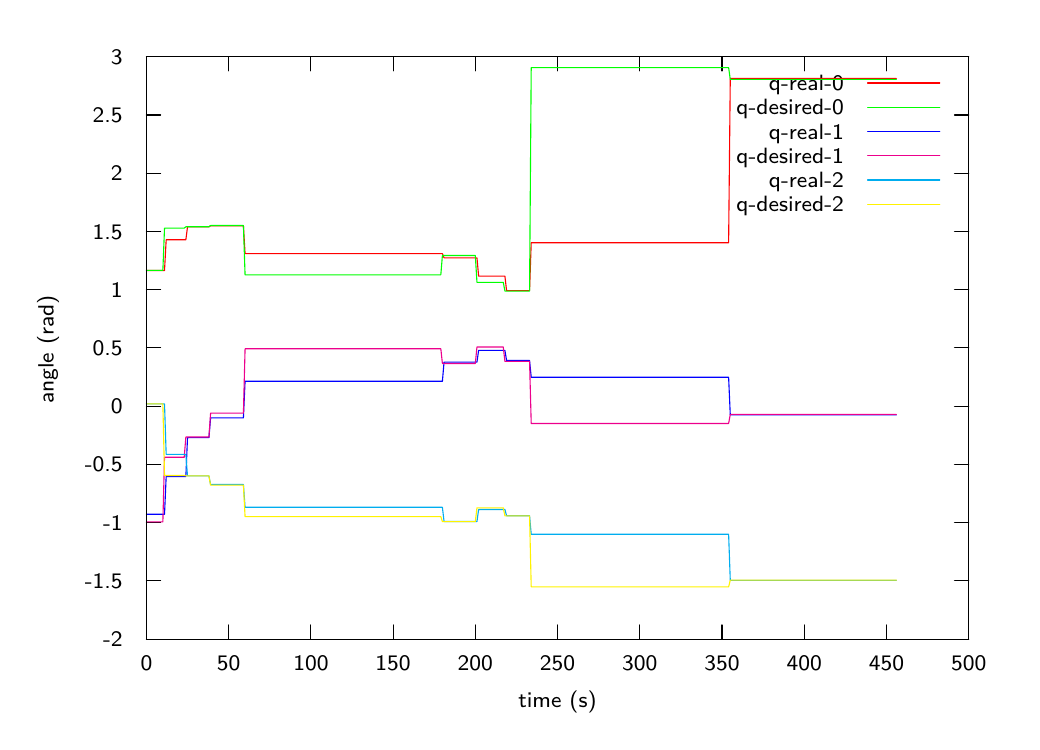
\begin{tikzpicture}[gnuplot]
%% generated with GNUPLOT 4.6p4 (Lua 5.1; terminal rev. 99, script rev. 100)
%% Thu 28 May 2015 12:34:40 AM CEST
\path (0.000,0.000) rectangle (12.500,8.750);
\gpcolor{color=gp lt color border}
\gpsetlinetype{gp lt border}
\gpsetlinewidth{1.00}
\draw[gp path] (1.504,0.985)--(1.684,0.985);
\draw[gp path] (11.947,0.985)--(11.767,0.985);
\node[gp node right,font={\fontsize{8pt}{9.6pt}\selectfont}] at (1.320,0.985) {-2};
\draw[gp path] (1.504,1.725)--(1.684,1.725);
\draw[gp path] (11.947,1.725)--(11.767,1.725);
\node[gp node right,font={\fontsize{8pt}{9.6pt}\selectfont}] at (1.320,1.725) {-1.5};
\draw[gp path] (1.504,2.464)--(1.684,2.464);
\draw[gp path] (11.947,2.464)--(11.767,2.464);
\node[gp node right,font={\fontsize{8pt}{9.6pt}\selectfont}] at (1.320,2.464) {-1};
\draw[gp path] (1.504,3.204)--(1.684,3.204);
\draw[gp path] (11.947,3.204)--(11.767,3.204);
\node[gp node right,font={\fontsize{8pt}{9.6pt}\selectfont}] at (1.320,3.204) {-0.5};
\draw[gp path] (1.504,3.943)--(1.684,3.943);
\draw[gp path] (11.947,3.943)--(11.767,3.943);
\node[gp node right,font={\fontsize{8pt}{9.6pt}\selectfont}] at (1.320,3.943) { 0};
\draw[gp path] (1.504,4.683)--(1.684,4.683);
\draw[gp path] (11.947,4.683)--(11.767,4.683);
\node[gp node right,font={\fontsize{8pt}{9.6pt}\selectfont}] at (1.320,4.683) { 0.5};
\draw[gp path] (1.504,5.423)--(1.684,5.423);
\draw[gp path] (11.947,5.423)--(11.767,5.423);
\node[gp node right,font={\fontsize{8pt}{9.6pt}\selectfont}] at (1.320,5.423) { 1};
\draw[gp path] (1.504,6.162)--(1.684,6.162);
\draw[gp path] (11.947,6.162)--(11.767,6.162);
\node[gp node right,font={\fontsize{8pt}{9.6pt}\selectfont}] at (1.320,6.162) { 1.5};
\draw[gp path] (1.504,6.902)--(1.684,6.902);
\draw[gp path] (11.947,6.902)--(11.767,6.902);
\node[gp node right,font={\fontsize{8pt}{9.6pt}\selectfont}] at (1.320,6.902) { 2};
\draw[gp path] (1.504,7.641)--(1.684,7.641);
\draw[gp path] (11.947,7.641)--(11.767,7.641);
\node[gp node right,font={\fontsize{8pt}{9.6pt}\selectfont}] at (1.320,7.641) { 2.5};
\draw[gp path] (1.504,8.381)--(1.684,8.381);
\draw[gp path] (11.947,8.381)--(11.767,8.381);
\node[gp node right,font={\fontsize{8pt}{9.6pt}\selectfont}] at (1.320,8.381) { 3};
\draw[gp path] (1.504,0.985)--(1.504,1.165);
\draw[gp path] (1.504,8.381)--(1.504,8.201);
\node[gp node center,font={\fontsize{8pt}{9.6pt}\selectfont}] at (1.504,0.677) { 0};
\draw[gp path] (2.548,0.985)--(2.548,1.165);
\draw[gp path] (2.548,8.381)--(2.548,8.201);
\node[gp node center,font={\fontsize{8pt}{9.6pt}\selectfont}] at (2.548,0.677) { 50};
\draw[gp path] (3.593,0.985)--(3.593,1.165);
\draw[gp path] (3.593,8.381)--(3.593,8.201);
\node[gp node center,font={\fontsize{8pt}{9.6pt}\selectfont}] at (3.593,0.677) { 100};
\draw[gp path] (4.637,0.985)--(4.637,1.165);
\draw[gp path] (4.637,8.381)--(4.637,8.201);
\node[gp node center,font={\fontsize{8pt}{9.6pt}\selectfont}] at (4.637,0.677) { 150};
\draw[gp path] (5.681,0.985)--(5.681,1.165);
\draw[gp path] (5.681,8.381)--(5.681,8.201);
\node[gp node center,font={\fontsize{8pt}{9.6pt}\selectfont}] at (5.681,0.677) { 200};
\draw[gp path] (6.726,0.985)--(6.726,1.165);
\draw[gp path] (6.726,8.381)--(6.726,8.201);
\node[gp node center,font={\fontsize{8pt}{9.6pt}\selectfont}] at (6.726,0.677) { 250};
\draw[gp path] (7.770,0.985)--(7.770,1.165);
\draw[gp path] (7.770,8.381)--(7.770,8.201);
\node[gp node center,font={\fontsize{8pt}{9.6pt}\selectfont}] at (7.770,0.677) { 300};
\draw[gp path] (8.814,0.985)--(8.814,1.165);
\draw[gp path] (8.814,8.381)--(8.814,8.201);
\node[gp node center,font={\fontsize{8pt}{9.6pt}\selectfont}] at (8.814,0.677) { 350};
\draw[gp path] (9.858,0.985)--(9.858,1.165);
\draw[gp path] (9.858,8.381)--(9.858,8.201);
\node[gp node center,font={\fontsize{8pt}{9.6pt}\selectfont}] at (9.858,0.677) { 400};
\draw[gp path] (10.903,0.985)--(10.903,1.165);
\draw[gp path] (10.903,8.381)--(10.903,8.201);
\node[gp node center,font={\fontsize{8pt}{9.6pt}\selectfont}] at (10.903,0.677) { 450};
\draw[gp path] (11.947,0.985)--(11.947,1.165);
\draw[gp path] (11.947,8.381)--(11.947,8.201);
\node[gp node center,font={\fontsize{8pt}{9.6pt}\selectfont}] at (11.947,0.677) { 500};
\draw[gp path] (1.504,8.381)--(1.504,0.985)--(11.947,0.985)--(11.947,8.381)--cycle;
\node[gp node center,rotate=-270,font={\fontsize{8pt}{9.6pt}\selectfont}] at (0.246,4.683) {angle (rad)};
\node[gp node center,font={\fontsize{8pt}{9.6pt}\selectfont}] at (6.725,0.215) {time (s)};
\node[gp node right,font={\fontsize{8pt}{9.6pt}\selectfont}] at (10.479,8.047) {q-real-0};
\gpcolor{color=gp lt color 0}
\gpsetlinetype{gp lt plot 0}
\draw[gp path] (10.663,8.047)--(11.579,8.047);
\draw[gp path] (1.504,5.666)--(1.525,5.666)--(1.546,5.666)--(1.567,5.666)--(1.588,5.666)%
  --(1.608,5.666)--(1.629,5.666)--(1.650,5.666)--(1.671,5.666)--(1.692,5.666)--(1.713,5.666)%
  --(1.734,5.666)--(1.755,6.056)--(1.776,6.056)--(1.796,6.056)--(1.817,6.056)--(1.838,6.056)%
  --(1.859,6.056)--(1.880,6.056)--(1.901,6.056)--(1.922,6.056)--(1.943,6.056)--(1.963,6.056)%
  --(1.984,6.056)--(2.005,6.056)--(2.026,6.220)--(2.047,6.220)--(2.068,6.220)--(2.089,6.220)%
  --(2.110,6.220)--(2.131,6.220)--(2.151,6.220)--(2.172,6.220)--(2.193,6.220)--(2.214,6.220)%
  --(2.235,6.220)--(2.256,6.220)--(2.277,6.220)--(2.298,6.220)--(2.319,6.235)--(2.339,6.235)%
  --(2.360,6.235)--(2.381,6.235)--(2.402,6.235)--(2.423,6.235)--(2.444,6.235)--(2.465,6.235)%
  --(2.486,6.235)--(2.507,6.235)--(2.527,6.235)--(2.548,6.235)--(2.569,6.235)--(2.590,6.235)%
  --(2.611,6.235)--(2.632,6.235)--(2.653,6.235)--(2.674,6.235)--(2.695,6.235)--(2.715,6.235)%
  --(2.736,6.235)--(2.757,5.881)--(2.778,5.881)--(2.799,5.881)--(2.820,5.881)--(2.841,5.881)%
  --(2.862,5.881)--(2.882,5.881)--(2.903,5.881)--(2.924,5.881)--(2.945,5.881)--(2.966,5.881)%
  --(2.987,5.881)--(3.008,5.881)--(3.029,5.881)--(3.050,5.881)--(3.070,5.881)--(3.091,5.881)%
  --(3.112,5.881)--(3.133,5.881)--(3.154,5.881)--(3.175,5.881)--(3.196,5.881)--(3.217,5.881)%
  --(3.238,5.881)--(3.258,5.881)--(3.279,5.881)--(3.300,5.881)--(3.321,5.881)--(3.342,5.881)%
  --(3.363,5.881)--(3.384,5.881)--(3.405,5.881)--(3.426,5.881)--(3.446,5.881)--(3.467,5.881)%
  --(3.488,5.881)--(3.509,5.881)--(3.530,5.881)--(3.551,5.881)--(3.572,5.881)--(3.593,5.881)%
  --(3.613,5.881)--(3.634,5.881)--(3.655,5.881)--(3.676,5.881)--(3.697,5.881)--(3.718,5.881)%
  --(3.739,5.881)--(3.760,5.881)--(3.781,5.881)--(3.801,5.881)--(3.822,5.881)--(3.843,5.881)%
  --(3.864,5.881)--(3.885,5.881)--(3.906,5.881)--(3.927,5.881)--(3.948,5.881)--(3.969,5.881)%
  --(3.989,5.881)--(4.010,5.881)--(4.031,5.881)--(4.052,5.881)--(4.073,5.881)--(4.094,5.881)%
  --(4.115,5.881)--(4.136,5.881)--(4.157,5.881)--(4.177,5.881)--(4.198,5.881)--(4.219,5.881)%
  --(4.240,5.881)--(4.261,5.881)--(4.282,5.881)--(4.303,5.881)--(4.324,5.881)--(4.344,5.881)%
  --(4.365,5.881)--(4.386,5.881)--(4.407,5.881)--(4.428,5.881)--(4.449,5.881)--(4.470,5.881)%
  --(4.491,5.881)--(4.512,5.881)--(4.532,5.881)--(4.553,5.881)--(4.574,5.881)--(4.595,5.881)%
  --(4.616,5.881)--(4.637,5.881)--(4.658,5.881)--(4.679,5.881)--(4.700,5.881)--(4.720,5.881)%
  --(4.741,5.881)--(4.762,5.881)--(4.783,5.881)--(4.804,5.881)--(4.825,5.881)--(4.846,5.881)%
  --(4.867,5.881)--(4.888,5.881)--(4.908,5.881)--(4.929,5.881)--(4.950,5.881)--(4.971,5.881)%
  --(4.992,5.881)--(5.013,5.881)--(5.034,5.881)--(5.055,5.881)--(5.076,5.881)--(5.096,5.881)%
  --(5.117,5.881)--(5.138,5.881)--(5.159,5.881)--(5.180,5.881)--(5.201,5.881)--(5.222,5.881)%
  --(5.243,5.881)--(5.263,5.881)--(5.284,5.827)--(5.305,5.827)--(5.326,5.827)--(5.347,5.827)%
  --(5.368,5.827)--(5.389,5.827)--(5.410,5.827)--(5.431,5.827)--(5.451,5.827)--(5.472,5.827)%
  --(5.493,5.827)--(5.514,5.827)--(5.535,5.827)--(5.556,5.827)--(5.577,5.827)--(5.598,5.827)%
  --(5.619,5.827)--(5.639,5.827)--(5.660,5.827)--(5.681,5.827)--(5.702,5.827)--(5.723,5.594)%
  --(5.744,5.594)--(5.765,5.594)--(5.786,5.594)--(5.807,5.594)--(5.827,5.594)--(5.848,5.594)%
  --(5.869,5.594)--(5.890,5.594)--(5.911,5.594)--(5.932,5.594)--(5.953,5.594)--(5.974,5.594)%
  --(5.994,5.594)--(6.015,5.594)--(6.036,5.594)--(6.057,5.594)--(6.078,5.411)--(6.099,5.411)%
  --(6.120,5.411)--(6.141,5.411)--(6.162,5.411)--(6.182,5.411)--(6.203,5.411)--(6.224,5.411)%
  --(6.245,5.411)--(6.266,5.411)--(6.287,5.411)--(6.308,5.411)--(6.329,5.411)--(6.350,5.411)%
  --(6.370,5.411)--(6.391,6.019)--(6.412,6.019)--(6.433,6.019)--(6.454,6.019)--(6.475,6.019)%
  --(6.496,6.019)--(6.517,6.019)--(6.538,6.019)--(6.558,6.019)--(6.579,6.019)--(6.600,6.019)%
  --(6.621,6.019)--(6.642,6.019)--(6.663,6.019)--(6.684,6.019)--(6.705,6.019)--(6.726,6.019)%
  --(6.746,6.019)--(6.767,6.019)--(6.788,6.019)--(6.809,6.019)--(6.830,6.019)--(6.851,6.019)%
  --(6.872,6.019)--(6.893,6.019)--(6.913,6.019)--(6.934,6.019)--(6.955,6.019)--(6.976,6.019)%
  --(6.997,6.019)--(7.018,6.019)--(7.039,6.019)--(7.060,6.019)--(7.081,6.019)--(7.101,6.019)%
  --(7.122,6.019)--(7.143,6.019)--(7.164,6.019)--(7.185,6.019)--(7.206,6.019)--(7.227,6.019)%
  --(7.248,6.019)--(7.269,6.019)--(7.289,6.019)--(7.310,6.019)--(7.331,6.019)--(7.352,6.019)%
  --(7.373,6.019)--(7.394,6.019)--(7.415,6.019)--(7.436,6.019)--(7.457,6.019)--(7.477,6.019)%
  --(7.498,6.019)--(7.519,6.019)--(7.540,6.019)--(7.561,6.019)--(7.582,6.019)--(7.603,6.019)%
  --(7.624,6.019)--(7.644,6.019)--(7.665,6.019)--(7.686,6.019)--(7.707,6.019)--(7.728,6.019)%
  --(7.749,6.019)--(7.770,6.019)--(7.791,6.019)--(7.812,6.019)--(7.832,6.019)--(7.853,6.019)%
  --(7.874,6.019)--(7.895,6.019)--(7.916,6.019)--(7.937,6.019)--(7.958,6.019)--(7.979,6.019)%
  --(8.000,6.019)--(8.020,6.019)--(8.041,6.019)--(8.062,6.019)--(8.083,6.019)--(8.104,6.019)%
  --(8.125,6.019)--(8.146,6.019)--(8.167,6.019)--(8.188,6.019)--(8.208,6.019)--(8.229,6.019)%
  --(8.250,6.019)--(8.271,6.019)--(8.292,6.019)--(8.313,6.019)--(8.334,6.019)--(8.355,6.019)%
  --(8.375,6.019)--(8.396,6.019)--(8.417,6.019)--(8.438,6.019)--(8.459,6.019)--(8.480,6.019)%
  --(8.501,6.019)--(8.522,6.019)--(8.543,6.019)--(8.563,6.019)--(8.584,6.019)--(8.605,6.019)%
  --(8.626,6.019)--(8.647,6.019)--(8.668,6.019)--(8.689,6.019)--(8.710,6.019)--(8.731,6.019)%
  --(8.751,6.019)--(8.772,6.019)--(8.793,6.019)--(8.814,6.019)--(8.835,6.019)--(8.856,6.019)%
  --(8.877,6.019)--(8.898,6.019)--(8.919,8.104)--(8.939,8.104)--(8.960,8.104)--(8.981,8.104)%
  --(9.002,8.104)--(9.023,8.104)--(9.044,8.104)--(9.065,8.104)--(9.086,8.104)--(9.107,8.104)%
  --(9.127,8.104)--(9.148,8.104)--(9.169,8.104)--(9.190,8.104)--(9.211,8.104)--(9.232,8.104)%
  --(9.253,8.104)--(9.274,8.104)--(9.294,8.104)--(9.315,8.104)--(9.336,8.104)--(9.357,8.104)%
  --(9.378,8.104)--(9.399,8.104)--(9.420,8.104)--(9.441,8.104)--(9.462,8.104)--(9.482,8.104)%
  --(9.503,8.104)--(9.524,8.104)--(9.545,8.104)--(9.566,8.104)--(9.587,8.104)--(9.608,8.104)%
  --(9.629,8.104)--(9.650,8.104)--(9.670,8.104)--(9.691,8.104)--(9.712,8.104)--(9.733,8.104)%
  --(9.754,8.104)--(9.775,8.104)--(9.796,8.104)--(9.817,8.104)--(9.838,8.104)--(9.858,8.104)%
  --(9.879,8.104)--(9.900,8.104)--(9.921,8.104)--(9.942,8.104)--(9.963,8.104)--(9.984,8.104)%
  --(10.005,8.104)--(10.025,8.104)--(10.046,8.104)--(10.067,8.104)--(10.088,8.104)--(10.109,8.104)%
  --(10.130,8.104)--(10.151,8.104)--(10.172,8.104)--(10.193,8.104)--(10.213,8.104)--(10.234,8.104)%
  --(10.255,8.104)--(10.276,8.104)--(10.297,8.104)--(10.318,8.104)--(10.339,8.104)--(10.360,8.104)%
  --(10.381,8.104)--(10.401,8.104)--(10.422,8.104)--(10.443,8.104)--(10.464,8.104)--(10.485,8.104)%
  --(10.506,8.104)--(10.527,8.104)--(10.548,8.104)--(10.569,8.104)--(10.589,8.104)--(10.610,8.104)%
  --(10.631,8.104)--(10.652,8.104)--(10.673,8.104)--(10.694,8.104)--(10.715,8.104)--(10.736,8.104)%
  --(10.756,8.104)--(10.777,8.104)--(10.798,8.104)--(10.819,8.104)--(10.840,8.104)--(10.861,8.104)%
  --(10.882,8.104)--(10.903,8.104)--(10.924,8.104)--(10.944,8.104)--(10.965,8.104)--(10.986,8.104)%
  --(11.007,8.104)--(11.028,8.104);
\gpcolor{color=gp lt color border}
\node[gp node right,font={\fontsize{8pt}{9.6pt}\selectfont}] at (10.479,7.739) {q-desired-0};
\gpcolor{color=gp lt color 1}
\gpsetlinetype{gp lt plot 1}
\draw[gp path] (10.663,7.739)--(11.579,7.739);
\draw[gp path] (1.504,5.668)--(1.525,5.668)--(1.546,5.668)--(1.567,5.668)--(1.588,5.668)%
  --(1.608,5.668)--(1.629,5.668)--(1.650,5.668)--(1.671,5.668)--(1.692,5.668)--(1.713,5.668)%
  --(1.734,6.205)--(1.755,6.205)--(1.776,6.205)--(1.796,6.205)--(1.817,6.205)--(1.838,6.205)%
  --(1.859,6.205)--(1.880,6.205)--(1.901,6.205)--(1.922,6.205)--(1.943,6.205)--(1.963,6.205)%
  --(1.984,6.205)--(2.005,6.221)--(2.026,6.221)--(2.047,6.221)--(2.068,6.221)--(2.089,6.221)%
  --(2.110,6.221)--(2.131,6.221)--(2.151,6.221)--(2.172,6.221)--(2.193,6.221)--(2.214,6.221)%
  --(2.235,6.221)--(2.256,6.221)--(2.277,6.221)--(2.298,6.221)--(2.319,6.237)--(2.339,6.237)%
  --(2.360,6.237)--(2.381,6.237)--(2.402,6.237)--(2.423,6.237)--(2.444,6.237)--(2.465,6.237)%
  --(2.486,6.237)--(2.507,6.237)--(2.527,6.237)--(2.548,6.237)--(2.569,6.237)--(2.590,6.237)%
  --(2.611,6.237)--(2.632,6.237)--(2.653,6.237)--(2.674,6.237)--(2.695,6.237)--(2.715,6.237)%
  --(2.736,6.237)--(2.757,5.611)--(2.778,5.611)--(2.799,5.611)--(2.820,5.611)--(2.841,5.611)%
  --(2.862,5.611)--(2.882,5.611)--(2.903,5.611)--(2.924,5.611)--(2.945,5.611)--(2.966,5.611)%
  --(2.987,5.611)--(3.008,5.611)--(3.029,5.611)--(3.050,5.611)--(3.070,5.611)--(3.091,5.611)%
  --(3.112,5.611)--(3.133,5.611)--(3.154,5.611)--(3.175,5.611)--(3.196,5.611)--(3.217,5.611)%
  --(3.238,5.611)--(3.258,5.611)--(3.279,5.611)--(3.300,5.611)--(3.321,5.611)--(3.342,5.611)%
  --(3.363,5.611)--(3.384,5.611)--(3.405,5.611)--(3.426,5.611)--(3.446,5.611)--(3.467,5.611)%
  --(3.488,5.611)--(3.509,5.611)--(3.530,5.611)--(3.551,5.611)--(3.572,5.611)--(3.593,5.611)%
  --(3.613,5.611)--(3.634,5.611)--(3.655,5.611)--(3.676,5.611)--(3.697,5.611)--(3.718,5.611)%
  --(3.739,5.611)--(3.760,5.611)--(3.781,5.611)--(3.801,5.611)--(3.822,5.611)--(3.843,5.611)%
  --(3.864,5.611)--(3.885,5.611)--(3.906,5.611)--(3.927,5.611)--(3.948,5.611)--(3.969,5.611)%
  --(3.989,5.611)--(4.010,5.611)--(4.031,5.611)--(4.052,5.611)--(4.073,5.611)--(4.094,5.611)%
  --(4.115,5.611)--(4.136,5.611)--(4.157,5.611)--(4.177,5.611)--(4.198,5.611)--(4.219,5.611)%
  --(4.240,5.611)--(4.261,5.611)--(4.282,5.611)--(4.303,5.611)--(4.324,5.611)--(4.344,5.611)%
  --(4.365,5.611)--(4.386,5.611)--(4.407,5.611)--(4.428,5.611)--(4.449,5.611)--(4.470,5.611)%
  --(4.491,5.611)--(4.512,5.611)--(4.532,5.611)--(4.553,5.611)--(4.574,5.611)--(4.595,5.611)%
  --(4.616,5.611)--(4.637,5.611)--(4.658,5.611)--(4.679,5.611)--(4.700,5.611)--(4.720,5.611)%
  --(4.741,5.611)--(4.762,5.611)--(4.783,5.611)--(4.804,5.611)--(4.825,5.611)--(4.846,5.611)%
  --(4.867,5.611)--(4.888,5.611)--(4.908,5.611)--(4.929,5.611)--(4.950,5.611)--(4.971,5.611)%
  --(4.992,5.611)--(5.013,5.611)--(5.034,5.611)--(5.055,5.611)--(5.076,5.611)--(5.096,5.611)%
  --(5.117,5.611)--(5.138,5.611)--(5.159,5.611)--(5.180,5.611)--(5.201,5.611)--(5.222,5.611)%
  --(5.243,5.611)--(5.263,5.857)--(5.284,5.857)--(5.305,5.857)--(5.326,5.857)--(5.347,5.857)%
  --(5.368,5.857)--(5.389,5.857)--(5.410,5.857)--(5.431,5.857)--(5.451,5.857)--(5.472,5.857)%
  --(5.493,5.857)--(5.514,5.857)--(5.535,5.857)--(5.556,5.857)--(5.577,5.857)--(5.598,5.857)%
  --(5.619,5.857)--(5.639,5.857)--(5.660,5.857)--(5.681,5.857)--(5.702,5.516)--(5.723,5.516)%
  --(5.744,5.516)--(5.765,5.516)--(5.786,5.516)--(5.807,5.516)--(5.827,5.516)--(5.848,5.516)%
  --(5.869,5.516)--(5.890,5.516)--(5.911,5.516)--(5.932,5.516)--(5.953,5.516)--(5.974,5.516)%
  --(5.994,5.516)--(6.015,5.516)--(6.036,5.516)--(6.057,5.405)--(6.078,5.405)--(6.099,5.405)%
  --(6.120,5.405)--(6.141,5.405)--(6.162,5.405)--(6.182,5.405)--(6.203,5.405)--(6.224,5.405)%
  --(6.245,5.405)--(6.266,5.405)--(6.287,5.405)--(6.308,5.405)--(6.329,5.405)--(6.350,5.405)%
  --(6.370,5.405)--(6.391,8.243)--(6.412,8.243)--(6.433,8.243)--(6.454,8.243)--(6.475,8.243)%
  --(6.496,8.243)--(6.517,8.243)--(6.538,8.243)--(6.558,8.243)--(6.579,8.243)--(6.600,8.243)%
  --(6.621,8.243)--(6.642,8.243)--(6.663,8.243)--(6.684,8.243)--(6.705,8.243)--(6.726,8.243)%
  --(6.746,8.243)--(6.767,8.243)--(6.788,8.243)--(6.809,8.243)--(6.830,8.243)--(6.851,8.243)%
  --(6.872,8.243)--(6.893,8.243)--(6.913,8.243)--(6.934,8.243)--(6.955,8.243)--(6.976,8.243)%
  --(6.997,8.243)--(7.018,8.243)--(7.039,8.243)--(7.060,8.243)--(7.081,8.243)--(7.101,8.243)%
  --(7.122,8.243)--(7.143,8.243)--(7.164,8.243)--(7.185,8.243)--(7.206,8.243)--(7.227,8.243)%
  --(7.248,8.243)--(7.269,8.243)--(7.289,8.243)--(7.310,8.243)--(7.331,8.243)--(7.352,8.243)%
  --(7.373,8.243)--(7.394,8.243)--(7.415,8.243)--(7.436,8.243)--(7.457,8.243)--(7.477,8.243)%
  --(7.498,8.243)--(7.519,8.243)--(7.540,8.243)--(7.561,8.243)--(7.582,8.243)--(7.603,8.243)%
  --(7.624,8.243)--(7.644,8.243)--(7.665,8.243)--(7.686,8.243)--(7.707,8.243)--(7.728,8.243)%
  --(7.749,8.243)--(7.770,8.243)--(7.791,8.243)--(7.812,8.243)--(7.832,8.243)--(7.853,8.243)%
  --(7.874,8.243)--(7.895,8.243)--(7.916,8.243)--(7.937,8.243)--(7.958,8.243)--(7.979,8.243)%
  --(8.000,8.243)--(8.020,8.243)--(8.041,8.243)--(8.062,8.243)--(8.083,8.243)--(8.104,8.243)%
  --(8.125,8.243)--(8.146,8.243)--(8.167,8.243)--(8.188,8.243)--(8.208,8.243)--(8.229,8.243)%
  --(8.250,8.243)--(8.271,8.243)--(8.292,8.243)--(8.313,8.243)--(8.334,8.243)--(8.355,8.243)%
  --(8.375,8.243)--(8.396,8.243)--(8.417,8.243)--(8.438,8.243)--(8.459,8.243)--(8.480,8.243)%
  --(8.501,8.243)--(8.522,8.243)--(8.543,8.243)--(8.563,8.243)--(8.584,8.243)--(8.605,8.243)%
  --(8.626,8.243)--(8.647,8.243)--(8.668,8.243)--(8.689,8.243)--(8.710,8.243)--(8.731,8.243)%
  --(8.751,8.243)--(8.772,8.243)--(8.793,8.243)--(8.814,8.243)--(8.835,8.243)--(8.856,8.243)%
  --(8.877,8.243)--(8.898,8.243)--(8.919,8.093)--(8.939,8.093)--(8.960,8.093)--(8.981,8.093)%
  --(9.002,8.093)--(9.023,8.093)--(9.044,8.093)--(9.065,8.093)--(9.086,8.093)--(9.107,8.093)%
  --(9.127,8.093)--(9.148,8.093)--(9.169,8.093)--(9.190,8.093)--(9.211,8.093)--(9.232,8.093)%
  --(9.253,8.093)--(9.274,8.093)--(9.294,8.093)--(9.315,8.093)--(9.336,8.093)--(9.357,8.093)%
  --(9.378,8.093)--(9.399,8.093)--(9.420,8.093)--(9.441,8.093)--(9.462,8.093)--(9.482,8.093)%
  --(9.503,8.093)--(9.524,8.093)--(9.545,8.093)--(9.566,8.093)--(9.587,8.093)--(9.608,8.093)%
  --(9.629,8.093)--(9.650,8.093)--(9.670,8.093)--(9.691,8.093)--(9.712,8.093)--(9.733,8.093)%
  --(9.754,8.093)--(9.775,8.093)--(9.796,8.093)--(9.817,8.093)--(9.838,8.093)--(9.858,8.093)%
  --(9.879,8.093)--(9.900,8.093)--(9.921,8.093)--(9.942,8.093)--(9.963,8.093)--(9.984,8.093)%
  --(10.005,8.093)--(10.025,8.093)--(10.046,8.093)--(10.067,8.093)--(10.088,8.093)--(10.109,8.093)%
  --(10.130,8.093)--(10.151,8.093)--(10.172,8.093)--(10.193,8.093)--(10.213,8.093)--(10.234,8.093)%
  --(10.255,8.093)--(10.276,8.093)--(10.297,8.093)--(10.318,8.093)--(10.339,8.093)--(10.360,8.093)%
  --(10.381,8.093)--(10.401,8.093)--(10.422,8.093)--(10.443,8.093)--(10.464,8.093)--(10.485,8.093)%
  --(10.506,8.093)--(10.527,8.093)--(10.548,8.093)--(10.569,8.093)--(10.589,8.093)--(10.610,8.093)%
  --(10.631,8.093)--(10.652,8.093)--(10.673,8.093)--(10.694,8.093)--(10.715,8.093)--(10.736,8.093)%
  --(10.756,8.093)--(10.777,8.093)--(10.798,8.093)--(10.819,8.093)--(10.840,8.093)--(10.861,8.093)%
  --(10.882,8.093)--(10.903,8.093)--(10.924,8.093)--(10.944,8.093)--(10.965,8.093)--(10.986,8.093)%
  --(11.007,8.093)--(11.028,8.093);
\gpcolor{color=gp lt color border}
\node[gp node right,font={\fontsize{8pt}{9.6pt}\selectfont}] at (10.479,7.431) {q-real-1};
\gpcolor{color=gp lt color 2}
\gpsetlinetype{gp lt plot 2}
\draw[gp path] (10.663,7.431)--(11.579,7.431);
\draw[gp path] (1.504,2.570)--(1.525,2.570)--(1.546,2.570)--(1.567,2.570)--(1.588,2.570)%
  --(1.608,2.570)--(1.629,2.570)--(1.650,2.570)--(1.671,2.570)--(1.692,2.570)--(1.713,2.570)%
  --(1.734,2.570)--(1.755,3.050)--(1.776,3.050)--(1.796,3.050)--(1.817,3.050)--(1.838,3.050)%
  --(1.859,3.050)--(1.880,3.050)--(1.901,3.050)--(1.922,3.050)--(1.943,3.050)--(1.963,3.050)%
  --(1.984,3.050)--(2.005,3.050)--(2.026,3.543)--(2.047,3.543)--(2.068,3.543)--(2.089,3.543)%
  --(2.110,3.543)--(2.131,3.543)--(2.151,3.543)--(2.172,3.543)--(2.193,3.543)--(2.214,3.543)%
  --(2.235,3.543)--(2.256,3.543)--(2.277,3.543)--(2.298,3.543)--(2.319,3.795)--(2.339,3.795)%
  --(2.360,3.795)--(2.381,3.795)--(2.402,3.795)--(2.423,3.795)--(2.444,3.795)--(2.465,3.795)%
  --(2.486,3.795)--(2.507,3.795)--(2.527,3.795)--(2.548,3.795)--(2.569,3.795)--(2.590,3.795)%
  --(2.611,3.795)--(2.632,3.795)--(2.653,3.795)--(2.674,3.795)--(2.695,3.795)--(2.715,3.795)%
  --(2.736,3.795)--(2.757,4.259)--(2.778,4.259)--(2.799,4.259)--(2.820,4.259)--(2.841,4.259)%
  --(2.862,4.259)--(2.882,4.259)--(2.903,4.259)--(2.924,4.259)--(2.945,4.259)--(2.966,4.259)%
  --(2.987,4.259)--(3.008,4.259)--(3.029,4.259)--(3.050,4.259)--(3.070,4.259)--(3.091,4.259)%
  --(3.112,4.259)--(3.133,4.259)--(3.154,4.259)--(3.175,4.259)--(3.196,4.259)--(3.217,4.259)%
  --(3.238,4.259)--(3.258,4.259)--(3.279,4.259)--(3.300,4.259)--(3.321,4.259)--(3.342,4.259)%
  --(3.363,4.259)--(3.384,4.259)--(3.405,4.259)--(3.426,4.259)--(3.446,4.259)--(3.467,4.259)%
  --(3.488,4.259)--(3.509,4.259)--(3.530,4.259)--(3.551,4.259)--(3.572,4.259)--(3.593,4.259)%
  --(3.613,4.259)--(3.634,4.259)--(3.655,4.259)--(3.676,4.259)--(3.697,4.259)--(3.718,4.259)%
  --(3.739,4.259)--(3.760,4.259)--(3.781,4.259)--(3.801,4.259)--(3.822,4.259)--(3.843,4.259)%
  --(3.864,4.259)--(3.885,4.259)--(3.906,4.259)--(3.927,4.259)--(3.948,4.259)--(3.969,4.259)%
  --(3.989,4.259)--(4.010,4.259)--(4.031,4.259)--(4.052,4.259)--(4.073,4.259)--(4.094,4.259)%
  --(4.115,4.259)--(4.136,4.259)--(4.157,4.259)--(4.177,4.259)--(4.198,4.259)--(4.219,4.259)%
  --(4.240,4.259)--(4.261,4.259)--(4.282,4.259)--(4.303,4.259)--(4.324,4.259)--(4.344,4.259)%
  --(4.365,4.259)--(4.386,4.259)--(4.407,4.259)--(4.428,4.259)--(4.449,4.259)--(4.470,4.259)%
  --(4.491,4.259)--(4.512,4.259)--(4.532,4.259)--(4.553,4.259)--(4.574,4.259)--(4.595,4.259)%
  --(4.616,4.259)--(4.637,4.259)--(4.658,4.259)--(4.679,4.259)--(4.700,4.259)--(4.720,4.259)%
  --(4.741,4.259)--(4.762,4.259)--(4.783,4.259)--(4.804,4.259)--(4.825,4.259)--(4.846,4.259)%
  --(4.867,4.259)--(4.888,4.259)--(4.908,4.259)--(4.929,4.259)--(4.950,4.259)--(4.971,4.259)%
  --(4.992,4.259)--(5.013,4.259)--(5.034,4.259)--(5.055,4.259)--(5.076,4.259)--(5.096,4.259)%
  --(5.117,4.259)--(5.138,4.259)--(5.159,4.259)--(5.180,4.259)--(5.201,4.259)--(5.222,4.259)%
  --(5.243,4.259)--(5.263,4.259)--(5.284,4.503)--(5.305,4.503)--(5.326,4.503)--(5.347,4.503)%
  --(5.368,4.503)--(5.389,4.503)--(5.410,4.503)--(5.431,4.503)--(5.451,4.503)--(5.472,4.503)%
  --(5.493,4.503)--(5.514,4.503)--(5.535,4.503)--(5.556,4.503)--(5.577,4.503)--(5.598,4.503)%
  --(5.619,4.503)--(5.639,4.503)--(5.660,4.503)--(5.681,4.503)--(5.702,4.503)--(5.723,4.651)%
  --(5.744,4.651)--(5.765,4.651)--(5.786,4.651)--(5.807,4.651)--(5.827,4.651)--(5.848,4.651)%
  --(5.869,4.651)--(5.890,4.651)--(5.911,4.651)--(5.932,4.651)--(5.953,4.651)--(5.974,4.651)%
  --(5.994,4.651)--(6.015,4.651)--(6.036,4.651)--(6.057,4.651)--(6.078,4.523)--(6.099,4.523)%
  --(6.120,4.523)--(6.141,4.523)--(6.162,4.523)--(6.182,4.523)--(6.203,4.523)--(6.224,4.523)%
  --(6.245,4.523)--(6.266,4.523)--(6.287,4.523)--(6.308,4.523)--(6.329,4.523)--(6.350,4.523)%
  --(6.370,4.523)--(6.391,4.311)--(6.412,4.311)--(6.433,4.311)--(6.454,4.311)--(6.475,4.311)%
  --(6.496,4.311)--(6.517,4.311)--(6.538,4.311)--(6.558,4.311)--(6.579,4.311)--(6.600,4.311)%
  --(6.621,4.311)--(6.642,4.311)--(6.663,4.311)--(6.684,4.311)--(6.705,4.311)--(6.726,4.311)%
  --(6.746,4.311)--(6.767,4.311)--(6.788,4.311)--(6.809,4.311)--(6.830,4.311)--(6.851,4.311)%
  --(6.872,4.311)--(6.893,4.311)--(6.913,4.311)--(6.934,4.311)--(6.955,4.311)--(6.976,4.311)%
  --(6.997,4.311)--(7.018,4.311)--(7.039,4.311)--(7.060,4.311)--(7.081,4.311)--(7.101,4.311)%
  --(7.122,4.311)--(7.143,4.311)--(7.164,4.311)--(7.185,4.311)--(7.206,4.311)--(7.227,4.311)%
  --(7.248,4.311)--(7.269,4.311)--(7.289,4.311)--(7.310,4.311)--(7.331,4.311)--(7.352,4.311)%
  --(7.373,4.311)--(7.394,4.311)--(7.415,4.311)--(7.436,4.311)--(7.457,4.311)--(7.477,4.311)%
  --(7.498,4.311)--(7.519,4.311)--(7.540,4.311)--(7.561,4.311)--(7.582,4.311)--(7.603,4.311)%
  --(7.624,4.311)--(7.644,4.311)--(7.665,4.311)--(7.686,4.311)--(7.707,4.311)--(7.728,4.311)%
  --(7.749,4.311)--(7.770,4.311)--(7.791,4.311)--(7.812,4.311)--(7.832,4.311)--(7.853,4.311)%
  --(7.874,4.311)--(7.895,4.311)--(7.916,4.311)--(7.937,4.311)--(7.958,4.311)--(7.979,4.311)%
  --(8.000,4.311)--(8.020,4.311)--(8.041,4.311)--(8.062,4.311)--(8.083,4.311)--(8.104,4.311)%
  --(8.125,4.311)--(8.146,4.311)--(8.167,4.311)--(8.188,4.311)--(8.208,4.311)--(8.229,4.311)%
  --(8.250,4.311)--(8.271,4.311)--(8.292,4.311)--(8.313,4.311)--(8.334,4.311)--(8.355,4.311)%
  --(8.375,4.311)--(8.396,4.311)--(8.417,4.311)--(8.438,4.311)--(8.459,4.311)--(8.480,4.311)%
  --(8.501,4.311)--(8.522,4.311)--(8.543,4.311)--(8.563,4.311)--(8.584,4.311)--(8.605,4.311)%
  --(8.626,4.311)--(8.647,4.311)--(8.668,4.311)--(8.689,4.311)--(8.710,4.311)--(8.731,4.311)%
  --(8.751,4.311)--(8.772,4.311)--(8.793,4.311)--(8.814,4.311)--(8.835,4.311)--(8.856,4.311)%
  --(8.877,4.311)--(8.898,4.311)--(8.919,3.832)--(8.939,3.832)--(8.960,3.832)--(8.981,3.832)%
  --(9.002,3.832)--(9.023,3.832)--(9.044,3.832)--(9.065,3.832)--(9.086,3.832)--(9.107,3.832)%
  --(9.127,3.832)--(9.148,3.832)--(9.169,3.832)--(9.190,3.832)--(9.211,3.832)--(9.232,3.832)%
  --(9.253,3.832)--(9.274,3.832)--(9.294,3.832)--(9.315,3.832)--(9.336,3.832)--(9.357,3.832)%
  --(9.378,3.832)--(9.399,3.832)--(9.420,3.832)--(9.441,3.832)--(9.462,3.832)--(9.482,3.832)%
  --(9.503,3.832)--(9.524,3.832)--(9.545,3.832)--(9.566,3.832)--(9.587,3.832)--(9.608,3.832)%
  --(9.629,3.832)--(9.650,3.832)--(9.670,3.832)--(9.691,3.832)--(9.712,3.832)--(9.733,3.832)%
  --(9.754,3.832)--(9.775,3.832)--(9.796,3.832)--(9.817,3.832)--(9.838,3.832)--(9.858,3.832)%
  --(9.879,3.832)--(9.900,3.832)--(9.921,3.832)--(9.942,3.832)--(9.963,3.832)--(9.984,3.832)%
  --(10.005,3.832)--(10.025,3.832)--(10.046,3.832)--(10.067,3.832)--(10.088,3.832)--(10.109,3.832)%
  --(10.130,3.832)--(10.151,3.832)--(10.172,3.832)--(10.193,3.832)--(10.213,3.832)--(10.234,3.832)%
  --(10.255,3.832)--(10.276,3.832)--(10.297,3.832)--(10.318,3.832)--(10.339,3.832)--(10.360,3.832)%
  --(10.381,3.832)--(10.401,3.832)--(10.422,3.832)--(10.443,3.832)--(10.464,3.832)--(10.485,3.832)%
  --(10.506,3.832)--(10.527,3.832)--(10.548,3.832)--(10.569,3.832)--(10.589,3.832)--(10.610,3.832)%
  --(10.631,3.832)--(10.652,3.832)--(10.673,3.832)--(10.694,3.832)--(10.715,3.832)--(10.736,3.832)%
  --(10.756,3.832)--(10.777,3.832)--(10.798,3.832)--(10.819,3.832)--(10.840,3.832)--(10.861,3.832)%
  --(10.882,3.832)--(10.903,3.832)--(10.924,3.832)--(10.944,3.832)--(10.965,3.832)--(10.986,3.832)%
  --(11.007,3.832)--(11.028,3.832);
\gpcolor{color=gp lt color border}
\node[gp node right,font={\fontsize{8pt}{9.6pt}\selectfont}] at (10.479,7.123) {q-desired-1};
\gpcolor{color=gp lt color 3}
\gpsetlinetype{gp lt plot 3}
\draw[gp path] (10.663,7.123)--(11.579,7.123);
\draw[gp path] (1.504,2.473)--(1.525,2.473)--(1.546,2.473)--(1.567,2.473)--(1.588,2.473)%
  --(1.608,2.473)--(1.629,2.473)--(1.650,2.473)--(1.671,2.473)--(1.692,2.473)--(1.713,2.473)%
  --(1.734,3.294)--(1.755,3.294)--(1.776,3.294)--(1.796,3.294)--(1.817,3.294)--(1.838,3.294)%
  --(1.859,3.294)--(1.880,3.294)--(1.901,3.294)--(1.922,3.294)--(1.943,3.294)--(1.963,3.294)%
  --(1.984,3.294)--(2.005,3.551)--(2.026,3.551)--(2.047,3.551)--(2.068,3.551)--(2.089,3.551)%
  --(2.110,3.551)--(2.131,3.551)--(2.151,3.551)--(2.172,3.551)--(2.193,3.551)--(2.214,3.551)%
  --(2.235,3.551)--(2.256,3.551)--(2.277,3.551)--(2.298,3.551)--(2.319,3.854)--(2.339,3.854)%
  --(2.360,3.854)--(2.381,3.854)--(2.402,3.854)--(2.423,3.854)--(2.444,3.854)--(2.465,3.854)%
  --(2.486,3.854)--(2.507,3.854)--(2.527,3.854)--(2.548,3.854)--(2.569,3.854)--(2.590,3.854)%
  --(2.611,3.854)--(2.632,3.854)--(2.653,3.854)--(2.674,3.854)--(2.695,3.854)--(2.715,3.854)%
  --(2.736,3.854)--(2.757,4.672)--(2.778,4.672)--(2.799,4.672)--(2.820,4.672)--(2.841,4.672)%
  --(2.862,4.672)--(2.882,4.672)--(2.903,4.672)--(2.924,4.672)--(2.945,4.672)--(2.966,4.672)%
  --(2.987,4.672)--(3.008,4.672)--(3.029,4.672)--(3.050,4.672)--(3.070,4.672)--(3.091,4.672)%
  --(3.112,4.672)--(3.133,4.672)--(3.154,4.672)--(3.175,4.672)--(3.196,4.672)--(3.217,4.672)%
  --(3.238,4.672)--(3.258,4.672)--(3.279,4.672)--(3.300,4.672)--(3.321,4.672)--(3.342,4.672)%
  --(3.363,4.672)--(3.384,4.672)--(3.405,4.672)--(3.426,4.672)--(3.446,4.672)--(3.467,4.672)%
  --(3.488,4.672)--(3.509,4.672)--(3.530,4.672)--(3.551,4.672)--(3.572,4.672)--(3.593,4.672)%
  --(3.613,4.672)--(3.634,4.672)--(3.655,4.672)--(3.676,4.672)--(3.697,4.672)--(3.718,4.672)%
  --(3.739,4.672)--(3.760,4.672)--(3.781,4.672)--(3.801,4.672)--(3.822,4.672)--(3.843,4.672)%
  --(3.864,4.672)--(3.885,4.672)--(3.906,4.672)--(3.927,4.672)--(3.948,4.672)--(3.969,4.672)%
  --(3.989,4.672)--(4.010,4.672)--(4.031,4.672)--(4.052,4.672)--(4.073,4.672)--(4.094,4.672)%
  --(4.115,4.672)--(4.136,4.672)--(4.157,4.672)--(4.177,4.672)--(4.198,4.672)--(4.219,4.672)%
  --(4.240,4.672)--(4.261,4.672)--(4.282,4.672)--(4.303,4.672)--(4.324,4.672)--(4.344,4.672)%
  --(4.365,4.672)--(4.386,4.672)--(4.407,4.672)--(4.428,4.672)--(4.449,4.672)--(4.470,4.672)%
  --(4.491,4.672)--(4.512,4.672)--(4.532,4.672)--(4.553,4.672)--(4.574,4.672)--(4.595,4.672)%
  --(4.616,4.672)--(4.637,4.672)--(4.658,4.672)--(4.679,4.672)--(4.700,4.672)--(4.720,4.672)%
  --(4.741,4.672)--(4.762,4.672)--(4.783,4.672)--(4.804,4.672)--(4.825,4.672)--(4.846,4.672)%
  --(4.867,4.672)--(4.888,4.672)--(4.908,4.672)--(4.929,4.672)--(4.950,4.672)--(4.971,4.672)%
  --(4.992,4.672)--(5.013,4.672)--(5.034,4.672)--(5.055,4.672)--(5.076,4.672)--(5.096,4.672)%
  --(5.117,4.672)--(5.138,4.672)--(5.159,4.672)--(5.180,4.672)--(5.201,4.672)--(5.222,4.672)%
  --(5.243,4.672)--(5.263,4.485)--(5.284,4.485)--(5.305,4.485)--(5.326,4.485)--(5.347,4.485)%
  --(5.368,4.485)--(5.389,4.485)--(5.410,4.485)--(5.431,4.485)--(5.451,4.485)--(5.472,4.485)%
  --(5.493,4.485)--(5.514,4.485)--(5.535,4.485)--(5.556,4.485)--(5.577,4.485)--(5.598,4.485)%
  --(5.619,4.485)--(5.639,4.485)--(5.660,4.485)--(5.681,4.485)--(5.702,4.694)--(5.723,4.694)%
  --(5.744,4.694)--(5.765,4.694)--(5.786,4.694)--(5.807,4.694)--(5.827,4.694)--(5.848,4.694)%
  --(5.869,4.694)--(5.890,4.694)--(5.911,4.694)--(5.932,4.694)--(5.953,4.694)--(5.974,4.694)%
  --(5.994,4.694)--(6.015,4.694)--(6.036,4.694)--(6.057,4.512)--(6.078,4.512)--(6.099,4.512)%
  --(6.120,4.512)--(6.141,4.512)--(6.162,4.512)--(6.182,4.512)--(6.203,4.512)--(6.224,4.512)%
  --(6.245,4.512)--(6.266,4.512)--(6.287,4.512)--(6.308,4.512)--(6.329,4.512)--(6.350,4.512)%
  --(6.370,4.512)--(6.391,3.723)--(6.412,3.723)--(6.433,3.723)--(6.454,3.723)--(6.475,3.723)%
  --(6.496,3.723)--(6.517,3.723)--(6.538,3.723)--(6.558,3.723)--(6.579,3.723)--(6.600,3.723)%
  --(6.621,3.723)--(6.642,3.723)--(6.663,3.723)--(6.684,3.723)--(6.705,3.723)--(6.726,3.723)%
  --(6.746,3.723)--(6.767,3.723)--(6.788,3.723)--(6.809,3.723)--(6.830,3.723)--(6.851,3.723)%
  --(6.872,3.723)--(6.893,3.723)--(6.913,3.723)--(6.934,3.723)--(6.955,3.723)--(6.976,3.723)%
  --(6.997,3.723)--(7.018,3.723)--(7.039,3.723)--(7.060,3.723)--(7.081,3.723)--(7.101,3.723)%
  --(7.122,3.723)--(7.143,3.723)--(7.164,3.723)--(7.185,3.723)--(7.206,3.723)--(7.227,3.723)%
  --(7.248,3.723)--(7.269,3.723)--(7.289,3.723)--(7.310,3.723)--(7.331,3.723)--(7.352,3.723)%
  --(7.373,3.723)--(7.394,3.723)--(7.415,3.723)--(7.436,3.723)--(7.457,3.723)--(7.477,3.723)%
  --(7.498,3.723)--(7.519,3.723)--(7.540,3.723)--(7.561,3.723)--(7.582,3.723)--(7.603,3.723)%
  --(7.624,3.723)--(7.644,3.723)--(7.665,3.723)--(7.686,3.723)--(7.707,3.723)--(7.728,3.723)%
  --(7.749,3.723)--(7.770,3.723)--(7.791,3.723)--(7.812,3.723)--(7.832,3.723)--(7.853,3.723)%
  --(7.874,3.723)--(7.895,3.723)--(7.916,3.723)--(7.937,3.723)--(7.958,3.723)--(7.979,3.723)%
  --(8.000,3.723)--(8.020,3.723)--(8.041,3.723)--(8.062,3.723)--(8.083,3.723)--(8.104,3.723)%
  --(8.125,3.723)--(8.146,3.723)--(8.167,3.723)--(8.188,3.723)--(8.208,3.723)--(8.229,3.723)%
  --(8.250,3.723)--(8.271,3.723)--(8.292,3.723)--(8.313,3.723)--(8.334,3.723)--(8.355,3.723)%
  --(8.375,3.723)--(8.396,3.723)--(8.417,3.723)--(8.438,3.723)--(8.459,3.723)--(8.480,3.723)%
  --(8.501,3.723)--(8.522,3.723)--(8.543,3.723)--(8.563,3.723)--(8.584,3.723)--(8.605,3.723)%
  --(8.626,3.723)--(8.647,3.723)--(8.668,3.723)--(8.689,3.723)--(8.710,3.723)--(8.731,3.723)%
  --(8.751,3.723)--(8.772,3.723)--(8.793,3.723)--(8.814,3.723)--(8.835,3.723)--(8.856,3.723)%
  --(8.877,3.723)--(8.898,3.723)--(8.919,3.838)--(8.939,3.838)--(8.960,3.838)--(8.981,3.838)%
  --(9.002,3.838)--(9.023,3.838)--(9.044,3.838)--(9.065,3.838)--(9.086,3.838)--(9.107,3.838)%
  --(9.127,3.838)--(9.148,3.838)--(9.169,3.838)--(9.190,3.838)--(9.211,3.838)--(9.232,3.838)%
  --(9.253,3.838)--(9.274,3.838)--(9.294,3.838)--(9.315,3.838)--(9.336,3.838)--(9.357,3.838)%
  --(9.378,3.838)--(9.399,3.838)--(9.420,3.838)--(9.441,3.838)--(9.462,3.838)--(9.482,3.838)%
  --(9.503,3.838)--(9.524,3.838)--(9.545,3.838)--(9.566,3.838)--(9.587,3.838)--(9.608,3.838)%
  --(9.629,3.838)--(9.650,3.838)--(9.670,3.838)--(9.691,3.838)--(9.712,3.838)--(9.733,3.838)%
  --(9.754,3.838)--(9.775,3.838)--(9.796,3.838)--(9.817,3.838)--(9.838,3.838)--(9.858,3.838)%
  --(9.879,3.838)--(9.900,3.838)--(9.921,3.838)--(9.942,3.838)--(9.963,3.838)--(9.984,3.838)%
  --(10.005,3.838)--(10.025,3.838)--(10.046,3.838)--(10.067,3.838)--(10.088,3.838)--(10.109,3.838)%
  --(10.130,3.838)--(10.151,3.838)--(10.172,3.838)--(10.193,3.838)--(10.213,3.838)--(10.234,3.838)%
  --(10.255,3.838)--(10.276,3.838)--(10.297,3.838)--(10.318,3.838)--(10.339,3.838)--(10.360,3.838)%
  --(10.381,3.838)--(10.401,3.838)--(10.422,3.838)--(10.443,3.838)--(10.464,3.838)--(10.485,3.838)%
  --(10.506,3.838)--(10.527,3.838)--(10.548,3.838)--(10.569,3.838)--(10.589,3.838)--(10.610,3.838)%
  --(10.631,3.838)--(10.652,3.838)--(10.673,3.838)--(10.694,3.838)--(10.715,3.838)--(10.736,3.838)%
  --(10.756,3.838)--(10.777,3.838)--(10.798,3.838)--(10.819,3.838)--(10.840,3.838)--(10.861,3.838)%
  --(10.882,3.838)--(10.903,3.838)--(10.924,3.838)--(10.944,3.838)--(10.965,3.838)--(10.986,3.838)%
  --(11.007,3.838)--(11.028,3.838);
\gpcolor{color=gp lt color border}
\node[gp node right,font={\fontsize{8pt}{9.6pt}\selectfont}] at (10.479,6.815) {q-real-2};
\gpcolor{color=gp lt color 4}
\gpsetlinetype{gp lt plot 4}
\draw[gp path] (10.663,6.815)--(11.579,6.815);
\draw[gp path] (1.504,3.972)--(1.525,3.972)--(1.546,3.972)--(1.567,3.972)--(1.588,3.972)%
  --(1.608,3.972)--(1.629,3.972)--(1.650,3.972)--(1.671,3.972)--(1.692,3.972)--(1.713,3.972)%
  --(1.734,3.972)--(1.755,3.331)--(1.776,3.331)--(1.796,3.331)--(1.817,3.331)--(1.838,3.331)%
  --(1.859,3.331)--(1.880,3.331)--(1.901,3.331)--(1.922,3.331)--(1.943,3.331)--(1.963,3.331)%
  --(1.984,3.331)--(2.005,3.331)--(2.026,3.057)--(2.047,3.057)--(2.068,3.057)--(2.089,3.057)%
  --(2.110,3.057)--(2.131,3.057)--(2.151,3.057)--(2.172,3.057)--(2.193,3.057)--(2.214,3.057)%
  --(2.235,3.057)--(2.256,3.057)--(2.277,3.057)--(2.298,3.057)--(2.319,2.948)--(2.339,2.948)%
  --(2.360,2.948)--(2.381,2.948)--(2.402,2.948)--(2.423,2.948)--(2.444,2.948)--(2.465,2.948)%
  --(2.486,2.948)--(2.507,2.948)--(2.527,2.948)--(2.548,2.948)--(2.569,2.948)--(2.590,2.948)%
  --(2.611,2.948)--(2.632,2.948)--(2.653,2.948)--(2.674,2.948)--(2.695,2.948)--(2.715,2.948)%
  --(2.736,2.948)--(2.757,2.659)--(2.778,2.659)--(2.799,2.659)--(2.820,2.659)--(2.841,2.659)%
  --(2.862,2.659)--(2.882,2.659)--(2.903,2.659)--(2.924,2.659)--(2.945,2.659)--(2.966,2.659)%
  --(2.987,2.659)--(3.008,2.659)--(3.029,2.659)--(3.050,2.659)--(3.070,2.659)--(3.091,2.659)%
  --(3.112,2.659)--(3.133,2.659)--(3.154,2.659)--(3.175,2.659)--(3.196,2.659)--(3.217,2.659)%
  --(3.238,2.659)--(3.258,2.659)--(3.279,2.659)--(3.300,2.659)--(3.321,2.659)--(3.342,2.659)%
  --(3.363,2.659)--(3.384,2.659)--(3.405,2.659)--(3.426,2.659)--(3.446,2.659)--(3.467,2.659)%
  --(3.488,2.659)--(3.509,2.659)--(3.530,2.659)--(3.551,2.659)--(3.572,2.659)--(3.593,2.659)%
  --(3.613,2.659)--(3.634,2.659)--(3.655,2.659)--(3.676,2.659)--(3.697,2.659)--(3.718,2.659)%
  --(3.739,2.659)--(3.760,2.659)--(3.781,2.659)--(3.801,2.659)--(3.822,2.659)--(3.843,2.659)%
  --(3.864,2.659)--(3.885,2.659)--(3.906,2.659)--(3.927,2.659)--(3.948,2.659)--(3.969,2.659)%
  --(3.989,2.659)--(4.010,2.659)--(4.031,2.659)--(4.052,2.659)--(4.073,2.659)--(4.094,2.659)%
  --(4.115,2.659)--(4.136,2.659)--(4.157,2.659)--(4.177,2.659)--(4.198,2.659)--(4.219,2.659)%
  --(4.240,2.659)--(4.261,2.659)--(4.282,2.659)--(4.303,2.659)--(4.324,2.659)--(4.344,2.659)%
  --(4.365,2.659)--(4.386,2.659)--(4.407,2.659)--(4.428,2.659)--(4.449,2.659)--(4.470,2.659)%
  --(4.491,2.659)--(4.512,2.659)--(4.532,2.659)--(4.553,2.659)--(4.574,2.659)--(4.595,2.659)%
  --(4.616,2.659)--(4.637,2.659)--(4.658,2.659)--(4.679,2.659)--(4.700,2.659)--(4.720,2.659)%
  --(4.741,2.659)--(4.762,2.659)--(4.783,2.659)--(4.804,2.659)--(4.825,2.659)--(4.846,2.659)%
  --(4.867,2.659)--(4.888,2.659)--(4.908,2.659)--(4.929,2.659)--(4.950,2.659)--(4.971,2.659)%
  --(4.992,2.659)--(5.013,2.659)--(5.034,2.659)--(5.055,2.659)--(5.076,2.659)--(5.096,2.659)%
  --(5.117,2.659)--(5.138,2.659)--(5.159,2.659)--(5.180,2.659)--(5.201,2.659)--(5.222,2.659)%
  --(5.243,2.659)--(5.263,2.659)--(5.284,2.479)--(5.305,2.479)--(5.326,2.479)--(5.347,2.479)%
  --(5.368,2.479)--(5.389,2.479)--(5.410,2.479)--(5.431,2.479)--(5.451,2.479)--(5.472,2.479)%
  --(5.493,2.479)--(5.514,2.479)--(5.535,2.479)--(5.556,2.479)--(5.577,2.479)--(5.598,2.479)%
  --(5.619,2.479)--(5.639,2.479)--(5.660,2.479)--(5.681,2.479)--(5.702,2.479)--(5.723,2.631)%
  --(5.744,2.631)--(5.765,2.631)--(5.786,2.631)--(5.807,2.631)--(5.827,2.631)--(5.848,2.631)%
  --(5.869,2.631)--(5.890,2.631)--(5.911,2.631)--(5.932,2.631)--(5.953,2.631)--(5.974,2.631)%
  --(5.994,2.631)--(6.015,2.631)--(6.036,2.631)--(6.057,2.631)--(6.078,2.552)--(6.099,2.552)%
  --(6.120,2.552)--(6.141,2.552)--(6.162,2.552)--(6.182,2.552)--(6.203,2.552)--(6.224,2.552)%
  --(6.245,2.552)--(6.266,2.552)--(6.287,2.552)--(6.308,2.552)--(6.329,2.552)--(6.350,2.552)%
  --(6.370,2.552)--(6.391,2.317)--(6.412,2.317)--(6.433,2.317)--(6.454,2.317)--(6.475,2.317)%
  --(6.496,2.317)--(6.517,2.317)--(6.538,2.317)--(6.558,2.317)--(6.579,2.317)--(6.600,2.317)%
  --(6.621,2.317)--(6.642,2.317)--(6.663,2.317)--(6.684,2.317)--(6.705,2.317)--(6.726,2.317)%
  --(6.746,2.317)--(6.767,2.317)--(6.788,2.317)--(6.809,2.317)--(6.830,2.317)--(6.851,2.317)%
  --(6.872,2.317)--(6.893,2.317)--(6.913,2.317)--(6.934,2.317)--(6.955,2.317)--(6.976,2.317)%
  --(6.997,2.317)--(7.018,2.317)--(7.039,2.317)--(7.060,2.317)--(7.081,2.317)--(7.101,2.317)%
  --(7.122,2.317)--(7.143,2.317)--(7.164,2.317)--(7.185,2.317)--(7.206,2.317)--(7.227,2.317)%
  --(7.248,2.317)--(7.269,2.317)--(7.289,2.317)--(7.310,2.317)--(7.331,2.317)--(7.352,2.317)%
  --(7.373,2.317)--(7.394,2.317)--(7.415,2.317)--(7.436,2.317)--(7.457,2.317)--(7.477,2.317)%
  --(7.498,2.317)--(7.519,2.317)--(7.540,2.317)--(7.561,2.317)--(7.582,2.317)--(7.603,2.317)%
  --(7.624,2.317)--(7.644,2.317)--(7.665,2.317)--(7.686,2.317)--(7.707,2.317)--(7.728,2.317)%
  --(7.749,2.317)--(7.770,2.317)--(7.791,2.317)--(7.812,2.317)--(7.832,2.317)--(7.853,2.317)%
  --(7.874,2.317)--(7.895,2.317)--(7.916,2.317)--(7.937,2.317)--(7.958,2.317)--(7.979,2.317)%
  --(8.000,2.317)--(8.020,2.317)--(8.041,2.317)--(8.062,2.317)--(8.083,2.317)--(8.104,2.317)%
  --(8.125,2.317)--(8.146,2.317)--(8.167,2.317)--(8.188,2.317)--(8.208,2.317)--(8.229,2.317)%
  --(8.250,2.317)--(8.271,2.317)--(8.292,2.317)--(8.313,2.317)--(8.334,2.317)--(8.355,2.317)%
  --(8.375,2.317)--(8.396,2.317)--(8.417,2.317)--(8.438,2.317)--(8.459,2.317)--(8.480,2.317)%
  --(8.501,2.317)--(8.522,2.317)--(8.543,2.317)--(8.563,2.317)--(8.584,2.317)--(8.605,2.317)%
  --(8.626,2.317)--(8.647,2.317)--(8.668,2.317)--(8.689,2.317)--(8.710,2.317)--(8.731,2.317)%
  --(8.751,2.317)--(8.772,2.317)--(8.793,2.317)--(8.814,2.317)--(8.835,2.317)--(8.856,2.317)%
  --(8.877,2.317)--(8.898,2.317)--(8.919,1.731)--(8.939,1.731)--(8.960,1.731)--(8.981,1.731)%
  --(9.002,1.731)--(9.023,1.731)--(9.044,1.731)--(9.065,1.731)--(9.086,1.731)--(9.107,1.731)%
  --(9.127,1.731)--(9.148,1.731)--(9.169,1.731)--(9.190,1.731)--(9.211,1.731)--(9.232,1.731)%
  --(9.253,1.731)--(9.274,1.731)--(9.294,1.731)--(9.315,1.731)--(9.336,1.731)--(9.357,1.731)%
  --(9.378,1.731)--(9.399,1.731)--(9.420,1.731)--(9.441,1.731)--(9.462,1.731)--(9.482,1.731)%
  --(9.503,1.731)--(9.524,1.731)--(9.545,1.731)--(9.566,1.731)--(9.587,1.731)--(9.608,1.731)%
  --(9.629,1.731)--(9.650,1.731)--(9.670,1.731)--(9.691,1.731)--(9.712,1.731)--(9.733,1.731)%
  --(9.754,1.731)--(9.775,1.731)--(9.796,1.731)--(9.817,1.731)--(9.838,1.731)--(9.858,1.731)%
  --(9.879,1.731)--(9.900,1.731)--(9.921,1.731)--(9.942,1.731)--(9.963,1.731)--(9.984,1.731)%
  --(10.005,1.731)--(10.025,1.731)--(10.046,1.731)--(10.067,1.731)--(10.088,1.731)--(10.109,1.731)%
  --(10.130,1.731)--(10.151,1.731)--(10.172,1.731)--(10.193,1.731)--(10.213,1.731)--(10.234,1.731)%
  --(10.255,1.731)--(10.276,1.731)--(10.297,1.731)--(10.318,1.731)--(10.339,1.731)--(10.360,1.731)%
  --(10.381,1.731)--(10.401,1.731)--(10.422,1.731)--(10.443,1.731)--(10.464,1.731)--(10.485,1.731)%
  --(10.506,1.731)--(10.527,1.731)--(10.548,1.731)--(10.569,1.731)--(10.589,1.731)--(10.610,1.731)%
  --(10.631,1.731)--(10.652,1.731)--(10.673,1.731)--(10.694,1.731)--(10.715,1.731)--(10.736,1.731)%
  --(10.756,1.731)--(10.777,1.731)--(10.798,1.731)--(10.819,1.731)--(10.840,1.731)--(10.861,1.731)%
  --(10.882,1.731)--(10.903,1.731)--(10.924,1.731)--(10.944,1.731)--(10.965,1.731)--(10.986,1.731)%
  --(11.007,1.731)--(11.028,1.731);
\gpcolor{color=gp lt color border}
\node[gp node right,font={\fontsize{8pt}{9.6pt}\selectfont}] at (10.479,6.507) {q-desired-2};
\gpcolor{color=gp lt color 5}
\gpsetlinetype{gp lt plot 5}
\draw[gp path] (10.663,6.507)--(11.579,6.507);
\draw[gp path] (1.504,3.973)--(1.525,3.973)--(1.546,3.973)--(1.567,3.973)--(1.588,3.973)%
  --(1.608,3.973)--(1.629,3.973)--(1.650,3.973)--(1.671,3.973)--(1.692,3.973)--(1.713,3.973)%
  --(1.734,3.063)--(1.755,3.063)--(1.776,3.063)--(1.796,3.063)--(1.817,3.063)--(1.838,3.063)%
  --(1.859,3.063)--(1.880,3.063)--(1.901,3.063)--(1.922,3.063)--(1.943,3.063)--(1.963,3.063)%
  --(1.984,3.063)--(2.005,3.057)--(2.026,3.057)--(2.047,3.057)--(2.068,3.057)--(2.089,3.057)%
  --(2.110,3.057)--(2.131,3.057)--(2.151,3.057)--(2.172,3.057)--(2.193,3.057)--(2.214,3.057)%
  --(2.235,3.057)--(2.256,3.057)--(2.277,3.057)--(2.298,3.057)--(2.319,2.940)--(2.339,2.940)%
  --(2.360,2.940)--(2.381,2.940)--(2.402,2.940)--(2.423,2.940)--(2.444,2.940)--(2.465,2.940)%
  --(2.486,2.940)--(2.507,2.940)--(2.527,2.940)--(2.548,2.940)--(2.569,2.940)--(2.590,2.940)%
  --(2.611,2.940)--(2.632,2.940)--(2.653,2.940)--(2.674,2.940)--(2.695,2.940)--(2.715,2.940)%
  --(2.736,2.940)--(2.757,2.540)--(2.778,2.540)--(2.799,2.540)--(2.820,2.540)--(2.841,2.540)%
  --(2.862,2.540)--(2.882,2.540)--(2.903,2.540)--(2.924,2.540)--(2.945,2.540)--(2.966,2.540)%
  --(2.987,2.540)--(3.008,2.540)--(3.029,2.540)--(3.050,2.540)--(3.070,2.540)--(3.091,2.540)%
  --(3.112,2.540)--(3.133,2.540)--(3.154,2.540)--(3.175,2.540)--(3.196,2.540)--(3.217,2.540)%
  --(3.238,2.540)--(3.258,2.540)--(3.279,2.540)--(3.300,2.540)--(3.321,2.540)--(3.342,2.540)%
  --(3.363,2.540)--(3.384,2.540)--(3.405,2.540)--(3.426,2.540)--(3.446,2.540)--(3.467,2.540)%
  --(3.488,2.540)--(3.509,2.540)--(3.530,2.540)--(3.551,2.540)--(3.572,2.540)--(3.593,2.540)%
  --(3.613,2.540)--(3.634,2.540)--(3.655,2.540)--(3.676,2.540)--(3.697,2.540)--(3.718,2.540)%
  --(3.739,2.540)--(3.760,2.540)--(3.781,2.540)--(3.801,2.540)--(3.822,2.540)--(3.843,2.540)%
  --(3.864,2.540)--(3.885,2.540)--(3.906,2.540)--(3.927,2.540)--(3.948,2.540)--(3.969,2.540)%
  --(3.989,2.540)--(4.010,2.540)--(4.031,2.540)--(4.052,2.540)--(4.073,2.540)--(4.094,2.540)%
  --(4.115,2.540)--(4.136,2.540)--(4.157,2.540)--(4.177,2.540)--(4.198,2.540)--(4.219,2.540)%
  --(4.240,2.540)--(4.261,2.540)--(4.282,2.540)--(4.303,2.540)--(4.324,2.540)--(4.344,2.540)%
  --(4.365,2.540)--(4.386,2.540)--(4.407,2.540)--(4.428,2.540)--(4.449,2.540)--(4.470,2.540)%
  --(4.491,2.540)--(4.512,2.540)--(4.532,2.540)--(4.553,2.540)--(4.574,2.540)--(4.595,2.540)%
  --(4.616,2.540)--(4.637,2.540)--(4.658,2.540)--(4.679,2.540)--(4.700,2.540)--(4.720,2.540)%
  --(4.741,2.540)--(4.762,2.540)--(4.783,2.540)--(4.804,2.540)--(4.825,2.540)--(4.846,2.540)%
  --(4.867,2.540)--(4.888,2.540)--(4.908,2.540)--(4.929,2.540)--(4.950,2.540)--(4.971,2.540)%
  --(4.992,2.540)--(5.013,2.540)--(5.034,2.540)--(5.055,2.540)--(5.076,2.540)--(5.096,2.540)%
  --(5.117,2.540)--(5.138,2.540)--(5.159,2.540)--(5.180,2.540)--(5.201,2.540)--(5.222,2.540)%
  --(5.243,2.540)--(5.263,2.477)--(5.284,2.477)--(5.305,2.477)--(5.326,2.477)--(5.347,2.477)%
  --(5.368,2.477)--(5.389,2.477)--(5.410,2.477)--(5.431,2.477)--(5.451,2.477)--(5.472,2.477)%
  --(5.493,2.477)--(5.514,2.477)--(5.535,2.477)--(5.556,2.477)--(5.577,2.477)--(5.598,2.477)%
  --(5.619,2.477)--(5.639,2.477)--(5.660,2.477)--(5.681,2.477)--(5.702,2.652)--(5.723,2.652)%
  --(5.744,2.652)--(5.765,2.652)--(5.786,2.652)--(5.807,2.652)--(5.827,2.652)--(5.848,2.652)%
  --(5.869,2.652)--(5.890,2.652)--(5.911,2.652)--(5.932,2.652)--(5.953,2.652)--(5.974,2.652)%
  --(5.994,2.652)--(6.015,2.652)--(6.036,2.652)--(6.057,2.549)--(6.078,2.549)--(6.099,2.549)%
  --(6.120,2.549)--(6.141,2.549)--(6.162,2.549)--(6.182,2.549)--(6.203,2.549)--(6.224,2.549)%
  --(6.245,2.549)--(6.266,2.549)--(6.287,2.549)--(6.308,2.549)--(6.329,2.549)--(6.350,2.549)%
  --(6.370,2.549)--(6.391,1.648)--(6.412,1.648)--(6.433,1.648)--(6.454,1.648)--(6.475,1.648)%
  --(6.496,1.648)--(6.517,1.648)--(6.538,1.648)--(6.558,1.648)--(6.579,1.648)--(6.600,1.648)%
  --(6.621,1.648)--(6.642,1.648)--(6.663,1.648)--(6.684,1.648)--(6.705,1.648)--(6.726,1.648)%
  --(6.746,1.648)--(6.767,1.648)--(6.788,1.648)--(6.809,1.648)--(6.830,1.648)--(6.851,1.648)%
  --(6.872,1.648)--(6.893,1.648)--(6.913,1.648)--(6.934,1.648)--(6.955,1.648)--(6.976,1.648)%
  --(6.997,1.648)--(7.018,1.648)--(7.039,1.648)--(7.060,1.648)--(7.081,1.648)--(7.101,1.648)%
  --(7.122,1.648)--(7.143,1.648)--(7.164,1.648)--(7.185,1.648)--(7.206,1.648)--(7.227,1.648)%
  --(7.248,1.648)--(7.269,1.648)--(7.289,1.648)--(7.310,1.648)--(7.331,1.648)--(7.352,1.648)%
  --(7.373,1.648)--(7.394,1.648)--(7.415,1.648)--(7.436,1.648)--(7.457,1.648)--(7.477,1.648)%
  --(7.498,1.648)--(7.519,1.648)--(7.540,1.648)--(7.561,1.648)--(7.582,1.648)--(7.603,1.648)%
  --(7.624,1.648)--(7.644,1.648)--(7.665,1.648)--(7.686,1.648)--(7.707,1.648)--(7.728,1.648)%
  --(7.749,1.648)--(7.770,1.648)--(7.791,1.648)--(7.812,1.648)--(7.832,1.648)--(7.853,1.648)%
  --(7.874,1.648)--(7.895,1.648)--(7.916,1.648)--(7.937,1.648)--(7.958,1.648)--(7.979,1.648)%
  --(8.000,1.648)--(8.020,1.648)--(8.041,1.648)--(8.062,1.648)--(8.083,1.648)--(8.104,1.648)%
  --(8.125,1.648)--(8.146,1.648)--(8.167,1.648)--(8.188,1.648)--(8.208,1.648)--(8.229,1.648)%
  --(8.250,1.648)--(8.271,1.648)--(8.292,1.648)--(8.313,1.648)--(8.334,1.648)--(8.355,1.648)%
  --(8.375,1.648)--(8.396,1.648)--(8.417,1.648)--(8.438,1.648)--(8.459,1.648)--(8.480,1.648)%
  --(8.501,1.648)--(8.522,1.648)--(8.543,1.648)--(8.563,1.648)--(8.584,1.648)--(8.605,1.648)%
  --(8.626,1.648)--(8.647,1.648)--(8.668,1.648)--(8.689,1.648)--(8.710,1.648)--(8.731,1.648)%
  --(8.751,1.648)--(8.772,1.648)--(8.793,1.648)--(8.814,1.648)--(8.835,1.648)--(8.856,1.648)%
  --(8.877,1.648)--(8.898,1.648)--(8.919,1.734)--(8.939,1.734)--(8.960,1.734)--(8.981,1.734)%
  --(9.002,1.734)--(9.023,1.734)--(9.044,1.734)--(9.065,1.734)--(9.086,1.734)--(9.107,1.734)%
  --(9.127,1.734)--(9.148,1.734)--(9.169,1.734)--(9.190,1.734)--(9.211,1.734)--(9.232,1.734)%
  --(9.253,1.734)--(9.274,1.734)--(9.294,1.734)--(9.315,1.734)--(9.336,1.734)--(9.357,1.734)%
  --(9.378,1.734)--(9.399,1.734)--(9.420,1.734)--(9.441,1.734)--(9.462,1.734)--(9.482,1.734)%
  --(9.503,1.734)--(9.524,1.734)--(9.545,1.734)--(9.566,1.734)--(9.587,1.734)--(9.608,1.734)%
  --(9.629,1.734)--(9.650,1.734)--(9.670,1.734)--(9.691,1.734)--(9.712,1.734)--(9.733,1.734)%
  --(9.754,1.734)--(9.775,1.734)--(9.796,1.734)--(9.817,1.734)--(9.838,1.734)--(9.858,1.734)%
  --(9.879,1.734)--(9.900,1.734)--(9.921,1.734)--(9.942,1.734)--(9.963,1.734)--(9.984,1.734)%
  --(10.005,1.734)--(10.025,1.734)--(10.046,1.734)--(10.067,1.734)--(10.088,1.734)--(10.109,1.734)%
  --(10.130,1.734)--(10.151,1.734)--(10.172,1.734)--(10.193,1.734)--(10.213,1.734)--(10.234,1.734)%
  --(10.255,1.734)--(10.276,1.734)--(10.297,1.734)--(10.318,1.734)--(10.339,1.734)--(10.360,1.734)%
  --(10.381,1.734)--(10.401,1.734)--(10.422,1.734)--(10.443,1.734)--(10.464,1.734)--(10.485,1.734)%
  --(10.506,1.734)--(10.527,1.734)--(10.548,1.734)--(10.569,1.734)--(10.589,1.734)--(10.610,1.734)%
  --(10.631,1.734)--(10.652,1.734)--(10.673,1.734)--(10.694,1.734)--(10.715,1.734)--(10.736,1.734)%
  --(10.756,1.734)--(10.777,1.734)--(10.798,1.734)--(10.819,1.734)--(10.840,1.734)--(10.861,1.734)%
  --(10.882,1.734)--(10.903,1.734)--(10.924,1.734)--(10.944,1.734)--(10.965,1.734)--(10.986,1.734)%
  --(11.007,1.734)--(11.028,1.734);
\gpcolor{color=gp lt color border}
\gpsetlinetype{gp lt border}
\draw[gp path] (1.504,8.381)--(1.504,0.985)--(11.947,0.985)--(11.947,8.381)--cycle;
%% coordinates of the plot area
\gpdefrectangularnode{gp plot 1}{\pgfpoint{1.504cm}{0.985cm}}{\pgfpoint{11.947cm}{8.381cm}}
\end{tikzpicture}
%% gnuplot variables

    }
    \caption{Real configuration as reported by the PA10 controller versus the desired configuration for the first 3 joints.}
    \label{fig:q_real_desired}
\end{figure}

In an optimal system the true and desired configurations should be the same, but here the results show otherwise.
Sometimes the robot does not adhere to the configuration sent to it, but stops after moving a little bit of the way.
The problem appears to happen when a desired joint angle is too far from the previous.
Some small part of the error might be explained by mechanical joint play, but it is much more likely that the PA10 controller is the culprit.

Further probing reveals that this problem is not common to PA10's but the particular one used in this project has an error.
At the time of writing, no measures have been taken to solve the problem, but one solution could be manually implementing a limit to how much a joint may be moved in on step.
If the desired move is greater than the limit, the system should split the move into several smaller ones.


% At the time of writing, the reason for the joint positional error is yet undetermined.

% Variation between the true and desired configuration might be caused by mechanical play of a particular joint.
% The play will have to be larger than the encoder resolution to be detected and thus significant.


\section{Precision of object detection}
Backprojection?


\section{Detected object position and Kalman filter estimate}
To show that the Kalman filter is working as expected, predicting the ball position even in cases where the detection algorithm fails momentarily, the following experiment is conducted.

The PA10 robot configuration and thus the camera position is kept constant.
The object to be tracked -- a ball -- is then moved slowly inside the view of the cameras.
At some point, the ball is obscured, so that the tracking algorithm no longer succeeds in detecting it.
That is the point at which the Kalman filter predictions become particularly important to keep track of the ball.
Especially so in cases where the ball would have otherwise moved out of sight of the cameras while obscured.

\begin{figure}[htb]
    \centering
    \begin{subfigure}[b]{0.49\textwidth}
        \resizebox{\columnwidth}{!}{%
            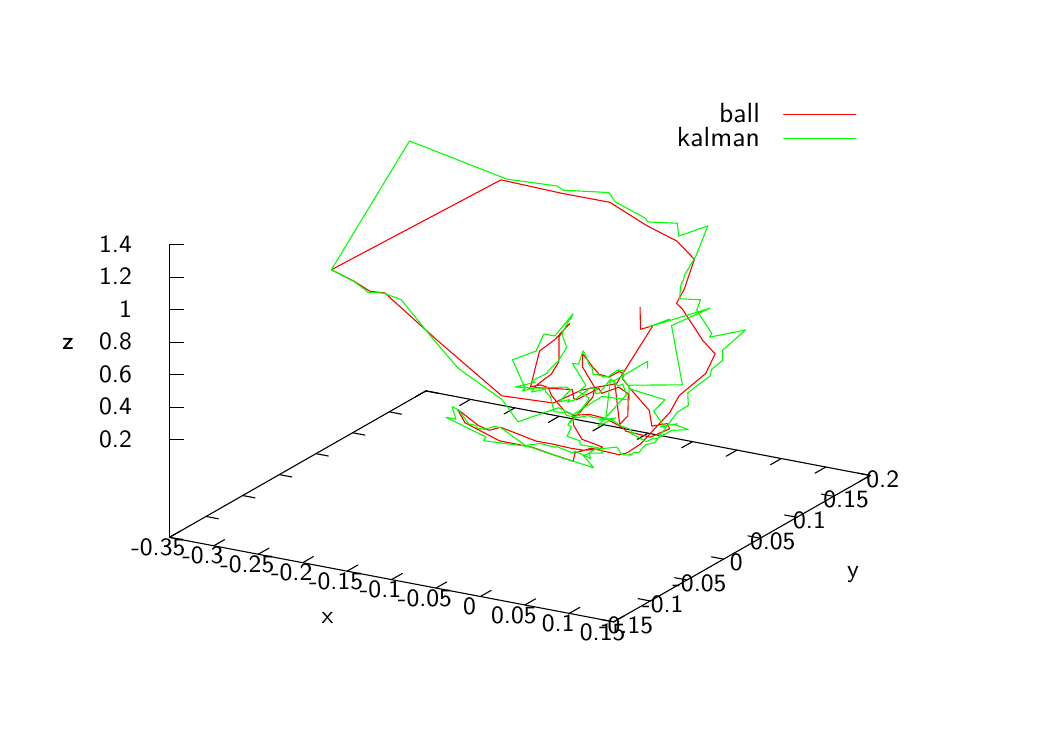
\begin{tikzpicture}[gnuplot]
%% generated with GNUPLOT 4.6p4 (Lua 5.1; terminal rev. 99, script rev. 100)
%% Wed 27 May 2015 02:02:52 AM CEST
\path (0.000,0.000) rectangle (12.500,8.750);
\gpcolor{color=gp lt color border}
\gpsetlinetype{gp lt border}
\gpsetlinewidth{1.00}
\draw[gp path] (1.800,2.277)--(5.058,4.137);
\draw[gp path] (10.700,3.063)--(5.058,4.137);
\draw[gp path] (1.800,2.277)--(1.800,5.995);
\draw[gp path] (1.800,2.277)--(1.937,2.355);
\node[gp node center,font={\fontsize{9pt}{10.8pt}\selectfont}] at (1.660,2.144) {-0.35};
\draw[gp path] (5.058,4.137)--(4.921,4.059);
\draw[gp path] (2.364,2.170)--(2.501,2.248);
\node[gp node center,font={\fontsize{9pt}{10.8pt}\selectfont}] at (2.225,2.036) {-0.3};
\draw[gp path] (5.622,4.029)--(5.486,3.951);
\draw[gp path] (2.929,2.063)--(3.065,2.140);
\node[gp node center,font={\fontsize{9pt}{10.8pt}\selectfont}] at (2.789,1.929) {-0.25};
\draw[gp path] (6.187,3.922)--(6.050,3.844);
\draw[gp path] (3.493,1.955)--(3.629,2.033);
\node[gp node center,font={\fontsize{9pt}{10.8pt}\selectfont}] at (3.353,1.822) {-0.2};
\draw[gp path] (6.750,3.815)--(6.613,3.737);
\draw[gp path] (4.057,1.848)--(4.194,1.926);
\node[gp node center,font={\fontsize{9pt}{10.8pt}\selectfont}] at (3.918,1.714) {-0.15};
\draw[gp path] (7.314,3.707)--(7.178,3.629);
\draw[gp path] (4.621,1.740)--(4.758,1.818);
\node[gp node center,font={\fontsize{9pt}{10.8pt}\selectfont}] at (4.482,1.607) {-0.1};
\draw[gp path] (7.878,3.600)--(7.742,3.522);
\draw[gp path] (5.186,1.633)--(5.322,1.711);
\node[gp node center,font={\fontsize{9pt}{10.8pt}\selectfont}] at (5.046,1.500) {-0.05};
\draw[gp path] (8.443,3.492)--(8.306,3.415);
\draw[gp path] (5.750,1.526)--(5.887,1.604);
\node[gp node center,font={\fontsize{9pt}{10.8pt}\selectfont}] at (5.610,1.392) { 0};
\draw[gp path] (9.007,3.385)--(8.871,3.307);
\draw[gp path] (6.313,1.418)--(6.450,1.496);
\node[gp node center,font={\fontsize{9pt}{10.8pt}\selectfont}] at (6.175,1.285) { 0.05};
\draw[gp path] (9.571,3.278)--(9.435,3.200);
\draw[gp path] (6.878,1.311)--(7.014,1.389);
\node[gp node center,font={\fontsize{9pt}{10.8pt}\selectfont}] at (6.738,1.178) { 0.1};
\draw[gp path] (10.136,3.170)--(9.999,3.092);
\draw[gp path] (7.442,1.204)--(7.579,1.282);
\node[gp node center,font={\fontsize{9pt}{10.8pt}\selectfont}] at (7.302,1.070) { 0.15};
\draw[gp path] (10.700,3.063)--(10.563,2.985);
\draw[gp path] (7.442,1.204)--(7.286,1.233);
\node[gp node center,font={\fontsize{9pt}{10.8pt}\selectfont}] at (7.601,1.153) {-0.15};
\draw[gp path] (1.800,2.277)--(1.956,2.248);
\draw[gp path] (7.907,1.469)--(7.752,1.499);
\node[gp node center,font={\fontsize{9pt}{10.8pt}\selectfont}] at (8.067,1.419) {-0.1};
\draw[gp path] (2.265,2.543)--(2.421,2.513);
\draw[gp path] (8.373,1.735)--(8.217,1.765);
\node[gp node center,font={\fontsize{9pt}{10.8pt}\selectfont}] at (8.532,1.684) {-0.05};
\draw[gp path] (2.731,2.808)--(2.887,2.779);
\draw[gp path] (8.838,2.001)--(8.682,2.030);
\node[gp node center,font={\fontsize{9pt}{10.8pt}\selectfont}] at (8.998,1.950) { 0};
\draw[gp path] (3.196,3.074)--(3.352,3.044);
\draw[gp path] (9.304,2.266)--(9.148,2.296);
\node[gp node center,font={\fontsize{9pt}{10.8pt}\selectfont}] at (9.463,2.215) { 0.05};
\draw[gp path] (3.662,3.340)--(3.818,3.310);
\draw[gp path] (9.769,2.532)--(9.613,2.561);
\node[gp node center,font={\fontsize{9pt}{10.8pt}\selectfont}] at (9.929,2.481) { 0.1};
\draw[gp path] (4.127,3.605)--(4.283,3.576);
\draw[gp path] (10.235,2.797)--(10.079,2.827);
\node[gp node center,font={\fontsize{9pt}{10.8pt}\selectfont}] at (10.394,2.747) { 0.15};
\draw[gp path] (4.593,3.871)--(4.748,3.841);
\draw[gp path] (10.700,3.063)--(10.544,3.093);
\node[gp node center,font={\fontsize{9pt}{10.8pt}\selectfont}] at (10.859,3.012) { 0.2};
\draw[gp path] (5.058,4.137)--(5.214,4.107);
\draw[gp path] (1.800,3.517)--(1.980,3.517);
\node[gp node right,font={\fontsize{9pt}{10.8pt}\selectfont}] at (1.440,3.517) { 0.2};
\draw[gp path] (1.800,3.930)--(1.980,3.930);
\node[gp node right,font={\fontsize{9pt}{10.8pt}\selectfont}] at (1.440,3.930) { 0.4};
\draw[gp path] (1.800,4.343)--(1.980,4.343);
\node[gp node right,font={\fontsize{9pt}{10.8pt}\selectfont}] at (1.440,4.343) { 0.6};
\draw[gp path] (1.800,4.755)--(1.980,4.755);
\node[gp node right,font={\fontsize{9pt}{10.8pt}\selectfont}] at (1.440,4.755) { 0.8};
\draw[gp path] (1.800,5.169)--(1.980,5.169);
\node[gp node right,font={\fontsize{9pt}{10.8pt}\selectfont}] at (1.440,5.169) { 1};
\draw[gp path] (1.800,5.582)--(1.980,5.582);
\node[gp node right,font={\fontsize{9pt}{10.8pt}\selectfont}] at (1.440,5.582) { 1.2};
\draw[gp path] (1.800,5.995)--(1.980,5.995);
\node[gp node right,font={\fontsize{9pt}{10.8pt}\selectfont}] at (1.440,5.995) { 1.4};
\node[gp node center,font={\fontsize{9pt}{10.8pt}\selectfont}] at (0.512,4.755) {z};
\node[gp node right] at (9.416,7.645) {ball};
\gpcolor{color=gp lt color 0}
\gpsetlinetype{gp lt plot 0}
\draw[gp path] (9.600,7.645)--(10.516,7.645);
\draw[gp path] (7.456,4.247)--(7.518,3.711)--(7.622,3.818)--(7.628,4.101)--(7.507,4.184)%
  --(7.291,4.106)--(7.253,4.168)--(6.968,4.023)--(6.935,4.039)--(6.918,4.154)--(6.433,4.180)%
  --(6.492,4.233)--(6.649,4.349)--(6.747,4.508)--(6.748,4.827)--(6.834,4.945)--(6.884,4.992)%
  --(6.692,4.786)--(6.501,4.644)--(6.387,4.191)--(6.514,4.212)--(6.610,4.180)--(6.654,4.077)%
  --(6.815,3.882)--(6.942,3.827)--(7.132,3.839)--(7.336,3.788)--(7.510,3.696)--(7.579,3.650)%
  --(7.597,3.625)--(7.909,3.550)--(8.151,3.655)--(8.123,3.721)--(7.927,3.690)--(7.895,3.888)%
  --(7.658,4.159)--(7.557,4.289)--(7.567,4.355)--(7.514,4.384)--(7.382,4.312)--(7.255,4.349)%
  --(7.173,4.445)--(7.049,4.608)--(7.045,4.444)--(7.199,4.183)--(7.179,4.060)--(7.014,3.864)%
  --(6.933,3.806)--(6.919,3.826)--(6.932,3.703)--(7.040,3.522)--(7.300,3.424)--(7.255,3.394)%
  --(7.055,3.384)--(6.887,3.411)--(6.660,3.463)--(6.461,3.498)--(6.007,3.675)--(5.860,3.637)%
  --(5.724,3.697)--(5.459,3.903)--(5.554,3.732)--(5.993,3.503)--(6.409,3.421)--(6.714,3.313)%
  --(6.929,3.244)--(6.950,3.349)--(7.160,3.409)--(7.515,3.325)--(7.591,3.343)--(7.636,3.365)%
  --(7.782,3.462)--(8.155,3.864)--(8.275,4.078)--(8.610,4.357)--(8.731,4.607)--(8.577,4.773)%
  --(8.315,5.176)--(8.239,5.249)--(8.338,5.427)--(8.467,5.808)--(8.246,6.039)--(7.854,6.241)%
  --(7.394,6.532)--(6.775,6.648)--(6.011,6.817)--(3.857,5.676)--(4.141,5.532)--(4.348,5.402)%
  --(4.535,5.381)--(5.210,4.772)--(6.020,4.075)--(6.677,3.983)--(7.032,4.147)--(7.478,4.230)%
  --(7.939,4.964)--(7.783,4.920)--(7.777,5.199);
\gpcolor{color=gp lt color border}
\node[gp node right] at (9.416,7.337) {kalman};
\gpcolor{color=gp lt color 1}
\gpsetlinetype{gp lt plot 1}
\draw[gp path] (9.600,7.337)--(10.516,7.337);
\draw[gp path] (7.874,4.426)--(7.873,4.469)--(7.871,4.511)--(7.454,4.268)--(7.400,4.280)%
  --(7.346,3.801)--(7.264,3.766)--(7.466,3.793)--(7.411,3.768)--(7.356,3.743)--(7.302,3.718)%
  --(7.244,3.691)--(7.603,4.088)--(7.598,4.103)--(7.593,4.118)--(7.588,4.133)--(7.583,4.148)%
  --(7.578,4.163)--(7.573,4.179)--(7.568,4.194)--(7.563,4.209)--(7.558,4.225)--(7.499,4.197)%
  --(7.487,4.208)--(7.476,4.220)--(7.464,4.231)--(7.452,4.243)--(7.440,4.254)--(7.428,4.266)%
  --(7.417,4.277)--(7.405,4.289)--(7.262,4.109)--(7.233,4.105)--(7.205,4.102)--(7.224,4.164)%
  --(7.205,4.167)--(7.186,4.171)--(7.167,4.175)--(7.149,4.179)--(6.943,4.021)--(6.899,4.008)%
  --(6.857,3.996)--(6.886,4.027)--(6.853,4.020)--(6.819,4.012)--(6.786,4.005)--(6.751,3.998)%
  --(6.894,4.152)--(6.881,4.160)--(6.868,4.168)--(6.854,4.177)--(6.841,4.186)--(6.452,4.172)%
  --(6.409,4.175)--(6.365,4.177)--(6.321,4.179)--(6.277,4.182)--(6.233,4.184)--(6.190,4.186)%
  --(6.441,4.246)--(6.421,4.256)--(6.402,4.265)--(6.603,4.364)--(6.606,4.385)--(6.738,4.519)%
  --(6.760,4.552)--(6.781,4.586)--(6.803,4.620)--(6.824,4.654)--(6.845,4.688)--(6.786,4.859)%
  --(6.804,4.901)--(6.849,4.982)--(6.871,5.027)--(6.893,5.072)--(6.894,5.042)--(6.910,5.080)%
  --(6.927,5.117)--(6.695,4.835)--(6.671,4.839)--(6.648,4.843)--(6.624,4.848)--(6.602,4.852)%
  --(6.579,4.856)--(6.556,4.860)--(6.456,4.643)--(6.418,4.629)--(6.381,4.615)--(6.344,4.601)%
  --(6.305,4.587)--(6.268,4.573)--(6.231,4.559)--(6.194,4.545)--(6.157,4.532)--(6.317,4.172)%
  --(6.280,4.135)--(6.433,4.176)--(6.417,4.149)--(6.401,4.123)--(6.572,4.159)--(6.576,4.140)%
  --(6.579,4.122)--(6.640,4.065)--(6.645,4.044)--(6.650,4.022)--(6.655,4.001)--(6.660,3.980)%
  --(6.664,3.958)--(6.670,3.936)--(6.675,3.915)--(6.680,3.893)--(6.685,3.872)--(6.821,3.863)%
  --(6.832,3.843)--(6.844,3.823)--(6.941,3.811)--(6.959,3.793)--(7.120,3.823)--(7.154,3.811)%
  --(7.189,3.799)--(7.346,3.784)--(7.387,3.774)--(7.429,3.764)--(7.533,3.693)--(7.575,3.678)%
  --(7.617,3.662)--(7.660,3.647)--(7.669,3.614)--(7.707,3.597)--(7.655,3.601)--(7.684,3.586)%
  --(7.714,3.570)--(7.743,3.555)--(7.772,3.539)--(7.801,3.524)--(7.830,3.508)--(7.861,3.492)%
  --(7.943,3.537)--(7.981,3.526)--(8.176,3.635)--(8.229,3.638)--(8.336,3.643)--(8.389,3.646)%
  --(8.210,3.713)--(8.250,3.720)--(8.037,3.684)--(8.051,3.682)--(8.064,3.680)--(8.078,3.678)%
  --(8.092,3.676)--(7.949,3.879)--(7.964,3.893)--(7.977,3.907)--(7.992,3.922)--(8.007,3.937)%
  --(8.022,3.953)--(8.036,3.967)--(8.050,3.982)--(8.064,3.996)--(8.078,4.010)--(8.092,4.025)%
  --(7.658,4.159)--(7.561,4.293)--(7.557,4.300)--(7.553,4.306)--(7.550,4.314)--(7.546,4.320)%
  --(7.569,4.362)--(7.568,4.372)--(7.568,4.382)--(7.567,4.391)--(7.566,4.401)--(7.515,4.392)%
  --(7.509,4.400)--(7.504,4.408)--(7.377,4.320)--(7.357,4.318)--(7.338,4.315)--(7.319,4.313)%
  --(7.246,4.343)--(7.225,4.343)--(7.204,4.343)--(7.182,4.343)--(7.165,4.442)--(7.149,4.451)%
  --(7.135,4.460)--(7.080,4.603)--(7.066,4.624)--(7.053,4.645)--(6.997,4.478)--(6.971,4.480)%
  --(6.945,4.483)--(6.919,4.485)--(7.089,4.208)--(7.065,4.187)--(7.043,4.167)--(7.019,4.146)%
  --(6.996,4.126)--(7.132,4.047)--(7.119,4.024)--(7.106,4.000)--(6.987,3.847)--(6.961,3.811)%
  --(6.935,3.775)--(6.912,3.768)--(6.887,3.733)--(6.909,3.780)--(6.892,3.756)--(6.876,3.731)%
  --(6.860,3.706)--(6.905,3.681)--(6.894,3.657)--(6.884,3.633)--(6.873,3.609)--(6.862,3.585)%
  --(6.851,3.560)--(7.014,3.503)--(7.015,3.478)--(7.016,3.453)--(7.251,3.414)--(7.270,3.391)%
  --(7.289,3.368)--(7.285,3.367)--(7.304,3.346)--(7.133,3.347)--(7.138,3.324)--(7.142,3.302)%
  --(7.147,3.279)--(6.946,3.374)--(6.939,3.360)--(6.931,3.347)--(6.718,3.429)--(6.697,3.421)%
  --(6.510,3.469)--(6.477,3.465)--(6.444,3.460)--(6.413,3.456)--(6.383,3.452)--(6.352,3.448)%
  --(6.321,3.444)--(6.014,3.666)--(5.972,3.677)--(5.930,3.687)--(5.806,3.650)--(5.758,3.656)%
  --(5.713,3.662)--(5.686,3.701)--(5.643,3.709)--(5.600,3.718)--(5.475,3.892)--(5.433,3.915)%
  --(5.391,3.937)--(5.438,3.778)--(5.396,3.786)--(5.352,3.794)--(5.312,3.802)--(5.822,3.550)%
  --(5.815,3.541)--(5.809,3.532)--(5.802,3.523)--(5.795,3.514)--(5.789,3.505)--(6.365,3.430)%
  --(6.395,3.420)--(6.425,3.409)--(6.453,3.400)--(6.701,3.317)--(6.742,3.303)--(6.783,3.289)%
  --(6.942,3.240)--(6.990,3.224)--(7.038,3.209)--(7.087,3.194)--(7.136,3.178)--(7.188,3.161)%
  --(7.050,3.322)--(7.081,3.318)--(7.201,3.395)--(7.240,3.399)--(7.280,3.403)--(7.322,3.407)%
  --(7.365,3.411)--(7.407,3.416)--(7.447,3.420)--(7.487,3.423)--(7.542,3.328)--(7.583,3.325)%
  --(7.623,3.323)--(7.664,3.320)--(7.645,3.336)--(7.681,3.334)--(7.695,3.356)--(7.731,3.356)%
  --(7.765,3.356)--(7.845,3.453)--(7.885,3.462)--(7.924,3.471)--(7.964,3.481)--(8.249,3.865)%
  --(8.319,3.909)--(8.390,3.954)--(8.383,4.112)--(8.458,4.170)--(8.529,4.224)--(8.600,4.277)%
  --(8.672,4.332)--(8.683,4.410)--(8.755,4.466)--(8.827,4.523)--(8.825,4.654)--(8.896,4.716)%
  --(8.971,4.782)--(9.047,4.849)--(9.118,4.911)--(8.660,4.819)--(8.690,4.864)--(8.497,5.162)%
  --(8.521,5.228)--(8.545,5.294)--(8.278,5.308)--(8.290,5.428)--(8.296,5.486)--(8.331,5.548)%
  --(8.339,5.602)--(8.488,5.854)--(8.518,5.929)--(8.548,6.004)--(8.577,6.078)--(8.607,6.153)%
  --(8.638,6.233)--(8.269,6.103)--(8.262,6.158)--(8.256,6.212)--(8.250,6.266)--(7.875,6.283)%
  --(7.844,6.331)--(7.464,6.537)--(7.422,6.596)--(7.379,6.656)--(6.805,6.686)--(6.719,6.740)%
  --(6.087,6.826)--(5.965,6.874)--(5.839,6.923)--(5.717,6.971)--(5.594,7.019)--(5.472,7.067)%
  --(5.351,7.115)--(5.230,7.162)--(5.101,7.212)--(4.970,7.263)--(4.849,7.311)--(3.857,5.676)%
  --(4.150,5.523)--(4.288,5.419)--(4.304,5.405)--(4.321,5.391)--(4.515,5.379)--(4.548,5.367)%
  --(4.582,5.355)--(4.614,5.343)--(4.646,5.332)--(4.677,5.321)--(4.709,5.309)--(4.741,5.298)%
  --(5.179,4.759)--(5.220,4.713)--(5.263,4.662)--(5.306,4.612)--(5.346,4.565)--(5.387,4.518)%
  --(5.427,4.471)--(5.468,4.424)--(6.023,4.028)--(6.124,3.887)--(6.227,3.744)--(6.741,3.923)%
  --(6.833,3.878)--(6.925,3.834)--(7.295,4.068)--(7.411,4.052)--(7.526,4.036)--(7.642,4.021)%
  --(7.634,4.209)--(7.761,4.210)--(7.880,4.211)--(8.000,4.212)--(8.193,4.213)--(8.315,4.214)%
  --(8.177,4.967)--(8.297,5.020)--(8.426,5.080)--(8.547,5.133)--(8.669,5.188)--(7.901,4.954)%
  --(7.964,4.978)--(8.027,5.002)--(8.090,5.026)--(8.152,5.049);
\gpcolor{color=gp lt color border}
\gpsetlinetype{gp lt border}
\draw[gp path] (10.700,3.063)--(7.442,1.204);
\draw[gp path] (1.800,2.277)--(7.442,1.204);
\node[gp node center,font={\fontsize{9pt}{10.8pt}\selectfont}] at (3.807,1.276) {x};
\node[gp node center,font={\fontsize{9pt}{10.8pt}\selectfont}] at (10.482,1.865) {y};
\node[gp node center,font={\fontsize{9pt}{10.8pt}\selectfont}] at (0.512,4.755) {z};
%% coordinates of the plot area
\gpdefrectangularnode{gp plot 1}{\pgfpoint{1.800cm}{0.771cm}}{\pgfpoint{10.700cm}{8.287cm}}
\end{tikzpicture}
%% gnuplot variables

        }
        \caption{Detected path of the ball and Kalman estimate.}
        \label{fig:ball_kalman_3d}
    \end{subfigure}~
    \begin{subfigure}[b]{0.49\textwidth}
        \resizebox{\columnwidth}{!}{%
            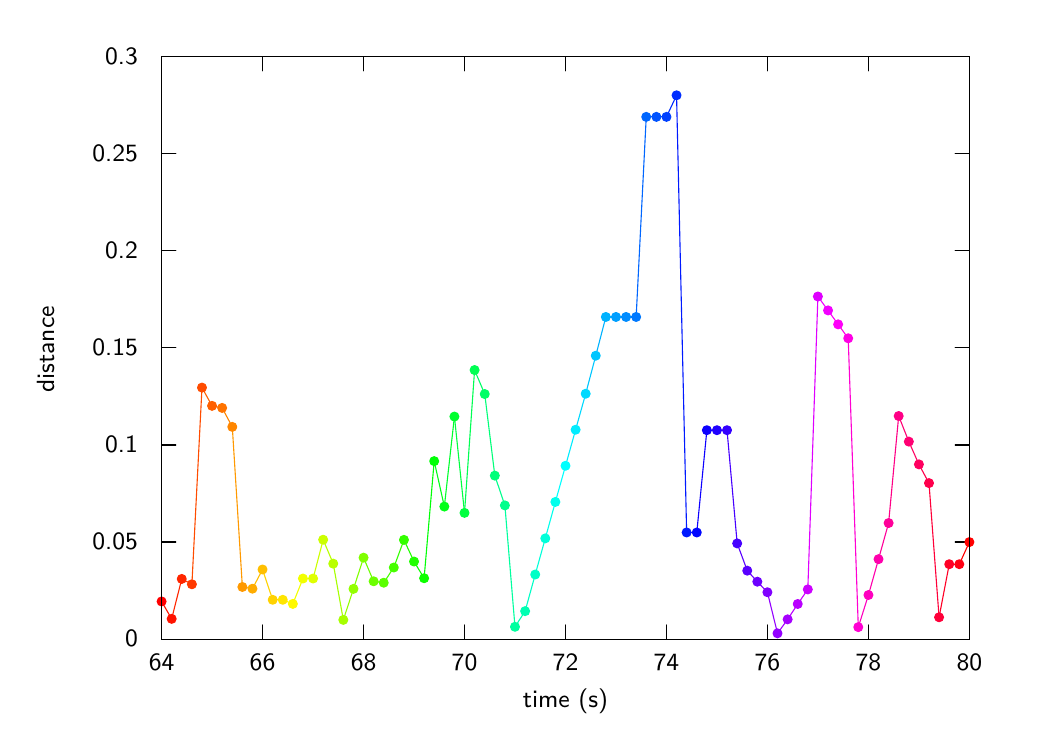
\begin{tikzpicture}[gnuplot]
%% generated with GNUPLOT 4.6p4 (Lua 5.1; terminal rev. 99, script rev. 100)
%% Thu 28 May 2015 09:06:58 AM CEST
\path (0.000,0.000) rectangle (12.500,8.750);
\gpcolor{color=gp lt color border}
\gpsetlinetype{gp lt border}
\gpsetlinewidth{1.00}
\draw[gp path] (1.688,0.985)--(1.868,0.985);
\draw[gp path] (11.947,0.985)--(11.767,0.985);
\node[gp node right,font={\fontsize{9pt}{10.8pt}\selectfont}] at (1.504,0.985) { 0};
\draw[gp path] (1.688,2.218)--(1.868,2.218);
\draw[gp path] (11.947,2.218)--(11.767,2.218);
\node[gp node right,font={\fontsize{9pt}{10.8pt}\selectfont}] at (1.504,2.218) { 0.05};
\draw[gp path] (1.688,3.450)--(1.868,3.450);
\draw[gp path] (11.947,3.450)--(11.767,3.450);
\node[gp node right,font={\fontsize{9pt}{10.8pt}\selectfont}] at (1.504,3.450) { 0.1};
\draw[gp path] (1.688,4.683)--(1.868,4.683);
\draw[gp path] (11.947,4.683)--(11.767,4.683);
\node[gp node right,font={\fontsize{9pt}{10.8pt}\selectfont}] at (1.504,4.683) { 0.15};
\draw[gp path] (1.688,5.916)--(1.868,5.916);
\draw[gp path] (11.947,5.916)--(11.767,5.916);
\node[gp node right,font={\fontsize{9pt}{10.8pt}\selectfont}] at (1.504,5.916) { 0.2};
\draw[gp path] (1.688,7.148)--(1.868,7.148);
\draw[gp path] (11.947,7.148)--(11.767,7.148);
\node[gp node right,font={\fontsize{9pt}{10.8pt}\selectfont}] at (1.504,7.148) { 0.25};
\draw[gp path] (1.688,8.381)--(1.868,8.381);
\draw[gp path] (11.947,8.381)--(11.767,8.381);
\node[gp node right,font={\fontsize{9pt}{10.8pt}\selectfont}] at (1.504,8.381) { 0.3};
\draw[gp path] (1.688,0.985)--(1.688,1.165);
\draw[gp path] (1.688,8.381)--(1.688,8.201);
\node[gp node center,font={\fontsize{9pt}{10.8pt}\selectfont}] at (1.688,0.677) { 64};
\draw[gp path] (2.970,0.985)--(2.970,1.165);
\draw[gp path] (2.970,8.381)--(2.970,8.201);
\node[gp node center,font={\fontsize{9pt}{10.8pt}\selectfont}] at (2.970,0.677) { 66};
\draw[gp path] (4.253,0.985)--(4.253,1.165);
\draw[gp path] (4.253,8.381)--(4.253,8.201);
\node[gp node center,font={\fontsize{9pt}{10.8pt}\selectfont}] at (4.253,0.677) { 68};
\draw[gp path] (5.535,0.985)--(5.535,1.165);
\draw[gp path] (5.535,8.381)--(5.535,8.201);
\node[gp node center,font={\fontsize{9pt}{10.8pt}\selectfont}] at (5.535,0.677) { 70};
\draw[gp path] (6.818,0.985)--(6.818,1.165);
\draw[gp path] (6.818,8.381)--(6.818,8.201);
\node[gp node center,font={\fontsize{9pt}{10.8pt}\selectfont}] at (6.818,0.677) { 72};
\draw[gp path] (8.100,0.985)--(8.100,1.165);
\draw[gp path] (8.100,8.381)--(8.100,8.201);
\node[gp node center,font={\fontsize{9pt}{10.8pt}\selectfont}] at (8.100,0.677) { 74};
\draw[gp path] (9.382,0.985)--(9.382,1.165);
\draw[gp path] (9.382,8.381)--(9.382,8.201);
\node[gp node center,font={\fontsize{9pt}{10.8pt}\selectfont}] at (9.382,0.677) { 76};
\draw[gp path] (10.665,0.985)--(10.665,1.165);
\draw[gp path] (10.665,8.381)--(10.665,8.201);
\node[gp node center,font={\fontsize{9pt}{10.8pt}\selectfont}] at (10.665,0.677) { 78};
\draw[gp path] (11.947,0.985)--(11.947,1.165);
\draw[gp path] (11.947,8.381)--(11.947,8.201);
\node[gp node center,font={\fontsize{9pt}{10.8pt}\selectfont}] at (11.947,0.677) { 80};
\draw[gp path] (1.688,8.381)--(1.688,0.985)--(11.947,0.985)--(11.947,8.381)--cycle;
\node[gp node center,rotate=-270,font={\fontsize{9pt}{10.8pt}\selectfont}] at (0.246,4.683) {distance};
\node[gp node center,font={\fontsize{9pt}{10.8pt}\selectfont}] at (6.817,0.215) {time (s)};
\gpcolor{rgb color={1.000,0.075,0.000}}
\gpsetlinetype{gp lt plot 0}
\draw[gp path] (1.688,1.463)--(1.816,1.242);
\gpcolor{rgb color={1.000,0.150,0.000}}
\draw[gp path] (1.816,1.242)--(1.944,1.749);
\gpcolor{rgb color={1.000,0.225,0.000}}
\draw[gp path] (1.944,1.749)--(2.073,1.681);
\gpcolor{rgb color={1.000,0.300,0.000}}
\draw[gp path] (2.073,1.681)--(2.201,4.179);
\gpcolor{rgb color={1.000,0.375,0.000}}
\draw[gp path] (2.201,4.179)--(2.329,3.947);
\gpcolor{rgb color={1.000,0.450,0.000}}
\draw[gp path] (2.329,3.947)--(2.457,3.921);
\gpcolor{rgb color={1.000,0.525,0.000}}
\draw[gp path] (2.457,3.921)--(2.586,3.680);
\gpcolor{rgb color={1.000,0.600,0.000}}
\draw[gp path] (2.586,3.680)--(2.714,1.647);
\gpcolor{rgb color={1.000,0.675,0.000}}
\draw[gp path] (2.714,1.647)--(2.842,1.625);
\gpcolor{rgb color={1.000,0.750,0.000}}
\draw[gp path] (2.842,1.625)--(2.970,1.869);
\gpcolor{rgb color={1.000,0.825,0.000}}
\draw[gp path] (2.970,1.869)--(3.099,1.484);
\gpcolor{rgb color={1.000,0.900,0.000}}
\draw[gp path] (3.099,1.484)--(3.227,1.484);
\gpcolor{rgb color={1.000,0.975,0.000}}
\draw[gp path] (3.227,1.484)--(3.355,1.432);
\gpcolor{rgb color={0.950,1.000,0.000}}
\draw[gp path] (3.355,1.432)--(3.483,1.754);
\gpcolor{rgb color={0.875,1.000,0.000}}
\draw[gp path] (3.483,1.754)--(3.612,1.754);
\gpcolor{rgb color={0.800,1.000,0.000}}
\draw[gp path] (3.612,1.754)--(3.740,2.247);
\gpcolor{rgb color={0.725,1.000,0.000}}
\draw[gp path] (3.740,2.247)--(3.868,1.943);
\gpcolor{rgb color={0.650,1.000,0.000}}
\draw[gp path] (3.868,1.943)--(3.996,1.229);
\gpcolor{rgb color={0.575,1.000,0.000}}
\draw[gp path] (3.996,1.229)--(4.125,1.623);
\gpcolor{rgb color={0.500,1.000,0.000}}
\draw[gp path] (4.125,1.623)--(4.253,2.019);
\gpcolor{rgb color={0.425,1.000,0.000}}
\draw[gp path] (4.253,2.019)--(4.381,1.719);
\gpcolor{rgb color={0.350,1.000,0.000}}
\draw[gp path] (4.381,1.719)--(4.509,1.701);
\gpcolor{rgb color={0.275,1.000,0.000}}
\draw[gp path] (4.509,1.701)--(4.637,1.894);
\gpcolor{rgb color={0.200,1.000,0.000}}
\draw[gp path] (4.637,1.894)--(4.766,2.245);
\gpcolor{rgb color={0.125,1.000,0.000}}
\draw[gp path] (4.766,2.245)--(4.894,1.970);
\gpcolor{rgb color={0.050,1.000,0.000}}
\draw[gp path] (4.894,1.970)--(5.022,1.758);
\gpcolor{rgb color={0.000,1.000,0.025}}
\draw[gp path] (5.022,1.758)--(5.150,3.245);
\gpcolor{rgb color={0.000,1.000,0.100}}
\draw[gp path] (5.150,3.245)--(5.279,2.668);
\gpcolor{rgb color={0.000,1.000,0.175}}
\draw[gp path] (5.279,2.668)--(5.407,3.811);
\gpcolor{rgb color={0.000,1.000,0.250}}
\draw[gp path] (5.407,3.811)--(5.535,2.588);
\gpcolor{rgb color={0.000,1.000,0.325}}
\draw[gp path] (5.535,2.588)--(5.663,4.402);
\gpcolor{rgb color={0.000,1.000,0.400}}
\draw[gp path] (5.663,4.402)--(5.792,4.097);
\gpcolor{rgb color={0.000,1.000,0.475}}
\draw[gp path] (5.792,4.097)--(5.920,3.061);
\gpcolor{rgb color={0.000,1.000,0.550}}
\draw[gp path] (5.920,3.061)--(6.048,2.683);
\gpcolor{rgb color={0.000,1.000,0.625}}
\draw[gp path] (6.048,2.683)--(6.176,1.141);
\gpcolor{rgb color={0.000,1.000,0.700}}
\draw[gp path] (6.176,1.141)--(6.305,1.340);
\gpcolor{rgb color={0.000,1.000,0.775}}
\draw[gp path] (6.305,1.340)--(6.433,1.805);
\gpcolor{rgb color={0.000,1.000,0.850}}
\draw[gp path] (6.433,1.805)--(6.561,2.264);
\gpcolor{rgb color={0.000,1.000,0.925}}
\draw[gp path] (6.561,2.264)--(6.689,2.727);
\gpcolor{rgb color={0.000,1.000,1.000}}
\draw[gp path] (6.689,2.727)--(6.818,3.186);
\gpcolor{rgb color={0.000,0.925,1.000}}
\draw[gp path] (6.818,3.186)--(6.946,3.644);
\gpcolor{rgb color={0.000,0.850,1.000}}
\draw[gp path] (6.946,3.644)--(7.074,4.101);
\gpcolor{rgb color={0.000,0.775,1.000}}
\draw[gp path] (7.074,4.101)--(7.202,4.584);
\gpcolor{rgb color={0.000,0.700,1.000}}
\draw[gp path] (7.202,4.584)--(7.330,5.076);
\gpcolor{rgb color={0.000,0.625,1.000}}
\draw[gp path] (7.330,5.076)--(7.459,5.076);
\gpcolor{rgb color={0.000,0.550,1.000}}
\draw[gp path] (7.459,5.076)--(7.587,5.076);
\gpcolor{rgb color={0.000,0.475,1.000}}
\draw[gp path] (7.587,5.076)--(7.715,5.076);
\gpcolor{rgb color={0.000,0.400,1.000}}
\draw[gp path] (7.715,5.076)--(7.843,7.617);
\gpcolor{rgb color={0.000,0.325,1.000}}
\draw[gp path] (7.843,7.617)--(7.972,7.617);
\gpcolor{rgb color={0.000,0.250,1.000}}
\draw[gp path] (7.972,7.617)--(8.100,7.617);
\gpcolor{rgb color={0.000,0.175,1.000}}
\draw[gp path] (8.100,7.617)--(8.228,7.891);
\gpcolor{rgb color={0.000,0.100,1.000}}
\draw[gp path] (8.228,7.891)--(8.356,2.339);
\gpcolor{rgb color={0.000,0.025,1.000}}
\draw[gp path] (8.356,2.339)--(8.485,2.339);
\gpcolor{rgb color={0.050,0.000,1.000}}
\draw[gp path] (8.485,2.339)--(8.613,3.638);
\gpcolor{rgb color={0.125,0.000,1.000}}
\draw[gp path] (8.613,3.638)--(8.741,3.638);
\gpcolor{rgb color={0.200,0.000,1.000}}
\draw[gp path] (8.741,3.638)--(8.869,3.638);
\gpcolor{rgb color={0.275,0.000,1.000}}
\draw[gp path] (8.869,3.638)--(8.998,2.200);
\gpcolor{rgb color={0.350,0.000,1.000}}
\draw[gp path] (8.998,2.200)--(9.126,1.854);
\gpcolor{rgb color={0.425,0.000,1.000}}
\draw[gp path] (9.126,1.854)--(9.254,1.714);
\gpcolor{rgb color={0.500,0.000,1.000}}
\draw[gp path] (9.254,1.714)--(9.382,1.580);
\gpcolor{rgb color={0.575,0.000,1.000}}
\draw[gp path] (9.382,1.580)--(9.510,1.058);
\gpcolor{rgb color={0.650,0.000,1.000}}
\draw[gp path] (9.510,1.058)--(9.639,1.236);
\gpcolor{rgb color={0.725,0.000,1.000}}
\draw[gp path] (9.639,1.236)--(9.767,1.431);
\gpcolor{rgb color={0.800,0.000,1.000}}
\draw[gp path] (9.767,1.431)--(9.895,1.616);
\gpcolor{rgb color={0.875,0.000,1.000}}
\draw[gp path] (9.895,1.616)--(10.023,5.336);
\gpcolor{rgb color={0.950,0.000,1.000}}
\draw[gp path] (10.023,5.336)--(10.152,5.159);
\gpcolor{rgb color={1.000,0.000,0.975}}
\draw[gp path] (10.152,5.159)--(10.280,4.982);
\gpcolor{rgb color={1.000,0.000,0.900}}
\draw[gp path] (10.280,4.982)--(10.408,4.805);
\gpcolor{rgb color={1.000,0.000,0.825}}
\draw[gp path] (10.408,4.805)--(10.536,1.137);
\gpcolor{rgb color={1.000,0.000,0.750}}
\draw[gp path] (10.536,1.137)--(10.665,1.545);
\gpcolor{rgb color={1.000,0.000,0.675}}
\draw[gp path] (10.665,1.545)--(10.793,2.000);
\gpcolor{rgb color={1.000,0.000,0.600}}
\draw[gp path] (10.793,2.000)--(10.921,2.459);
\gpcolor{rgb color={1.000,0.000,0.525}}
\draw[gp path] (10.921,2.459)--(11.049,3.818);
\gpcolor{rgb color={1.000,0.000,0.450}}
\draw[gp path] (11.049,3.818)--(11.178,3.493);
\gpcolor{rgb color={1.000,0.000,0.375}}
\draw[gp path] (11.178,3.493)--(11.306,3.204);
\gpcolor{rgb color={1.000,0.000,0.300}}
\draw[gp path] (11.306,3.204)--(11.434,2.966);
\gpcolor{rgb color={1.000,0.000,0.225}}
\draw[gp path] (11.434,2.966)--(11.562,1.262);
\gpcolor{rgb color={1.000,0.000,0.150}}
\draw[gp path] (11.562,1.262)--(11.691,1.936);
\gpcolor{rgb color={1.000,0.000,0.075}}
\draw[gp path] (11.691,1.936)--(11.819,1.936);
\gpcolor{rgb color={1.000,0.000,0.000}}
\draw[gp path] (11.819,1.936)--(11.947,2.217);
\gpsetpointsize{4.00}
\gppoint{gp mark 7}{(1.688,1.463)}
\gpcolor{rgb color={1.000,0.075,0.000}}
\gppoint{gp mark 7}{(1.816,1.242)}
\gpcolor{rgb color={1.000,0.150,0.000}}
\gppoint{gp mark 7}{(1.944,1.749)}
\gpcolor{rgb color={1.000,0.225,0.000}}
\gppoint{gp mark 7}{(2.073,1.681)}
\gpcolor{rgb color={1.000,0.300,0.000}}
\gppoint{gp mark 7}{(2.201,4.179)}
\gpcolor{rgb color={1.000,0.375,0.000}}
\gppoint{gp mark 7}{(2.329,3.947)}
\gpcolor{rgb color={1.000,0.450,0.000}}
\gppoint{gp mark 7}{(2.457,3.921)}
\gpcolor{rgb color={1.000,0.525,0.000}}
\gppoint{gp mark 7}{(2.586,3.680)}
\gpcolor{rgb color={1.000,0.600,0.000}}
\gppoint{gp mark 7}{(2.714,1.647)}
\gpcolor{rgb color={1.000,0.675,0.000}}
\gppoint{gp mark 7}{(2.842,1.625)}
\gpcolor{rgb color={1.000,0.750,0.000}}
\gppoint{gp mark 7}{(2.970,1.869)}
\gpcolor{rgb color={1.000,0.825,0.000}}
\gppoint{gp mark 7}{(3.099,1.484)}
\gpcolor{rgb color={1.000,0.900,0.000}}
\gppoint{gp mark 7}{(3.227,1.484)}
\gpcolor{rgb color={1.000,0.975,0.000}}
\gppoint{gp mark 7}{(3.355,1.432)}
\gpcolor{rgb color={0.950,1.000,0.000}}
\gppoint{gp mark 7}{(3.483,1.754)}
\gpcolor{rgb color={0.875,1.000,0.000}}
\gppoint{gp mark 7}{(3.612,1.754)}
\gpcolor{rgb color={0.800,1.000,0.000}}
\gppoint{gp mark 7}{(3.740,2.247)}
\gpcolor{rgb color={0.725,1.000,0.000}}
\gppoint{gp mark 7}{(3.868,1.943)}
\gpcolor{rgb color={0.650,1.000,0.000}}
\gppoint{gp mark 7}{(3.996,1.229)}
\gpcolor{rgb color={0.575,1.000,0.000}}
\gppoint{gp mark 7}{(4.125,1.623)}
\gpcolor{rgb color={0.500,1.000,0.000}}
\gppoint{gp mark 7}{(4.253,2.019)}
\gpcolor{rgb color={0.425,1.000,0.000}}
\gppoint{gp mark 7}{(4.381,1.719)}
\gpcolor{rgb color={0.350,1.000,0.000}}
\gppoint{gp mark 7}{(4.509,1.701)}
\gpcolor{rgb color={0.275,1.000,0.000}}
\gppoint{gp mark 7}{(4.637,1.894)}
\gpcolor{rgb color={0.200,1.000,0.000}}
\gppoint{gp mark 7}{(4.766,2.245)}
\gpcolor{rgb color={0.125,1.000,0.000}}
\gppoint{gp mark 7}{(4.894,1.970)}
\gpcolor{rgb color={0.050,1.000,0.000}}
\gppoint{gp mark 7}{(5.022,1.758)}
\gpcolor{rgb color={0.000,1.000,0.025}}
\gppoint{gp mark 7}{(5.150,3.245)}
\gpcolor{rgb color={0.000,1.000,0.100}}
\gppoint{gp mark 7}{(5.279,2.668)}
\gpcolor{rgb color={0.000,1.000,0.175}}
\gppoint{gp mark 7}{(5.407,3.811)}
\gpcolor{rgb color={0.000,1.000,0.250}}
\gppoint{gp mark 7}{(5.535,2.588)}
\gpcolor{rgb color={0.000,1.000,0.325}}
\gppoint{gp mark 7}{(5.663,4.402)}
\gpcolor{rgb color={0.000,1.000,0.400}}
\gppoint{gp mark 7}{(5.792,4.097)}
\gpcolor{rgb color={0.000,1.000,0.475}}
\gppoint{gp mark 7}{(5.920,3.061)}
\gpcolor{rgb color={0.000,1.000,0.550}}
\gppoint{gp mark 7}{(6.048,2.683)}
\gpcolor{rgb color={0.000,1.000,0.625}}
\gppoint{gp mark 7}{(6.176,1.141)}
\gpcolor{rgb color={0.000,1.000,0.700}}
\gppoint{gp mark 7}{(6.305,1.340)}
\gpcolor{rgb color={0.000,1.000,0.775}}
\gppoint{gp mark 7}{(6.433,1.805)}
\gpcolor{rgb color={0.000,1.000,0.850}}
\gppoint{gp mark 7}{(6.561,2.264)}
\gpcolor{rgb color={0.000,1.000,0.925}}
\gppoint{gp mark 7}{(6.689,2.727)}
\gpcolor{rgb color={0.000,1.000,1.000}}
\gppoint{gp mark 7}{(6.818,3.186)}
\gpcolor{rgb color={0.000,0.925,1.000}}
\gppoint{gp mark 7}{(6.946,3.644)}
\gpcolor{rgb color={0.000,0.850,1.000}}
\gppoint{gp mark 7}{(7.074,4.101)}
\gpcolor{rgb color={0.000,0.775,1.000}}
\gppoint{gp mark 7}{(7.202,4.584)}
\gpcolor{rgb color={0.000,0.700,1.000}}
\gppoint{gp mark 7}{(7.330,5.076)}
\gpcolor{rgb color={0.000,0.625,1.000}}
\gppoint{gp mark 7}{(7.459,5.076)}
\gpcolor{rgb color={0.000,0.550,1.000}}
\gppoint{gp mark 7}{(7.587,5.076)}
\gpcolor{rgb color={0.000,0.475,1.000}}
\gppoint{gp mark 7}{(7.715,5.076)}
\gpcolor{rgb color={0.000,0.400,1.000}}
\gppoint{gp mark 7}{(7.843,7.617)}
\gpcolor{rgb color={0.000,0.325,1.000}}
\gppoint{gp mark 7}{(7.972,7.617)}
\gpcolor{rgb color={0.000,0.250,1.000}}
\gppoint{gp mark 7}{(8.100,7.617)}
\gpcolor{rgb color={0.000,0.175,1.000}}
\gppoint{gp mark 7}{(8.228,7.891)}
\gpcolor{rgb color={0.000,0.100,1.000}}
\gppoint{gp mark 7}{(8.356,2.339)}
\gpcolor{rgb color={0.000,0.025,1.000}}
\gppoint{gp mark 7}{(8.485,2.339)}
\gpcolor{rgb color={0.050,0.000,1.000}}
\gppoint{gp mark 7}{(8.613,3.638)}
\gpcolor{rgb color={0.125,0.000,1.000}}
\gppoint{gp mark 7}{(8.741,3.638)}
\gpcolor{rgb color={0.200,0.000,1.000}}
\gppoint{gp mark 7}{(8.869,3.638)}
\gpcolor{rgb color={0.275,0.000,1.000}}
\gppoint{gp mark 7}{(8.998,2.200)}
\gpcolor{rgb color={0.350,0.000,1.000}}
\gppoint{gp mark 7}{(9.126,1.854)}
\gpcolor{rgb color={0.425,0.000,1.000}}
\gppoint{gp mark 7}{(9.254,1.714)}
\gpcolor{rgb color={0.500,0.000,1.000}}
\gppoint{gp mark 7}{(9.382,1.580)}
\gpcolor{rgb color={0.575,0.000,1.000}}
\gppoint{gp mark 7}{(9.510,1.058)}
\gpcolor{rgb color={0.650,0.000,1.000}}
\gppoint{gp mark 7}{(9.639,1.236)}
\gpcolor{rgb color={0.725,0.000,1.000}}
\gppoint{gp mark 7}{(9.767,1.431)}
\gpcolor{rgb color={0.800,0.000,1.000}}
\gppoint{gp mark 7}{(9.895,1.616)}
\gpcolor{rgb color={0.875,0.000,1.000}}
\gppoint{gp mark 7}{(10.023,5.336)}
\gpcolor{rgb color={0.950,0.000,1.000}}
\gppoint{gp mark 7}{(10.152,5.159)}
\gpcolor{rgb color={1.000,0.000,0.975}}
\gppoint{gp mark 7}{(10.280,4.982)}
\gpcolor{rgb color={1.000,0.000,0.900}}
\gppoint{gp mark 7}{(10.408,4.805)}
\gpcolor{rgb color={1.000,0.000,0.825}}
\gppoint{gp mark 7}{(10.536,1.137)}
\gpcolor{rgb color={1.000,0.000,0.750}}
\gppoint{gp mark 7}{(10.665,1.545)}
\gpcolor{rgb color={1.000,0.000,0.675}}
\gppoint{gp mark 7}{(10.793,2.000)}
\gpcolor{rgb color={1.000,0.000,0.600}}
\gppoint{gp mark 7}{(10.921,2.459)}
\gpcolor{rgb color={1.000,0.000,0.525}}
\gppoint{gp mark 7}{(11.049,3.818)}
\gpcolor{rgb color={1.000,0.000,0.450}}
\gppoint{gp mark 7}{(11.178,3.493)}
\gpcolor{rgb color={1.000,0.000,0.375}}
\gppoint{gp mark 7}{(11.306,3.204)}
\gpcolor{rgb color={1.000,0.000,0.300}}
\gppoint{gp mark 7}{(11.434,2.966)}
\gpcolor{rgb color={1.000,0.000,0.225}}
\gppoint{gp mark 7}{(11.562,1.262)}
\gpcolor{rgb color={1.000,0.000,0.150}}
\gppoint{gp mark 7}{(11.691,1.936)}
\gpcolor{rgb color={1.000,0.000,0.075}}
\gppoint{gp mark 7}{(11.819,1.936)}
\gpcolor{rgb color={1.000,0.000,0.000}}
\gppoint{gp mark 7}{(11.947,2.217)}
\gpcolor{color=gp lt color border}
\gpsetlinetype{gp lt border}
\draw[gp path] (1.688,8.381)--(1.688,0.985)--(11.947,0.985)--(11.947,8.381)--cycle;
%% coordinates of the plot area
\gpdefrectangularnode{gp plot 1}{\pgfpoint{1.688cm}{0.985cm}}{\pgfpoint{11.947cm}{8.381cm}}
\end{tikzpicture}
%% gnuplot variables

        }
        \caption{Positional difference between detected ball position and Kalman estimate.}
        \label{fig:ball_kalman_error}
    \end{subfigure}
    \caption{Detected ball positions and associated Kalman filter estimates.}
    \label{fig:kalman_test}
\end{figure}

Figure~\ref{fig:kalman_test} shows a 16 second extract of positional data gathered by the ball detection algorithm and Kalman filter.
Figure~\ref{fig:ball_kalman_3d} depicts the 3D positions while \ref{fig:ball_kalman_error} shows the difference between the last detected ball position and Kalman filter estimate. Associated measurements (at the same time) are the same color.

At 71 seconds the ball is no longer detected for approximately 3 seconds, so the ``detected'' position remains constant. The Kalman filter continues predicting the ball position based on previous samples however. This may be be seen in the error graph; the difference between detected ball position and the estimate grows quickly until around 74 seconds, where the ball is once again detected correctly in the camera images.

In general, whenever the ball changes direction, velocity or acceleration the error will increase because the Kalman filter is yet uncorrected. If the tracked object is not detected, the filter update step is skipped entirely.


\section{Paths planning around obstacles}
Simulation only



% \begin{figure}[htb]
%     \centering
%     \resizebox{\columnwidth}{!}{%
%         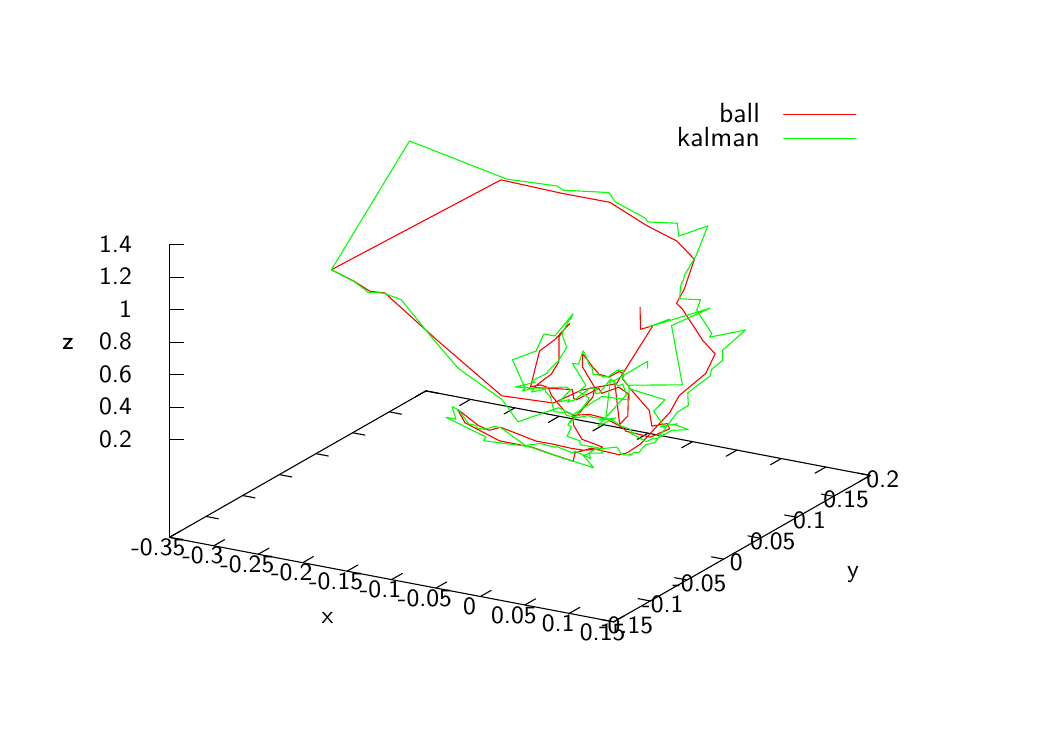
\begin{tikzpicture}[gnuplot]
%% generated with GNUPLOT 4.6p4 (Lua 5.1; terminal rev. 99, script rev. 100)
%% Wed 27 May 2015 02:02:52 AM CEST
\path (0.000,0.000) rectangle (12.500,8.750);
\gpcolor{color=gp lt color border}
\gpsetlinetype{gp lt border}
\gpsetlinewidth{1.00}
\draw[gp path] (1.800,2.277)--(5.058,4.137);
\draw[gp path] (10.700,3.063)--(5.058,4.137);
\draw[gp path] (1.800,2.277)--(1.800,5.995);
\draw[gp path] (1.800,2.277)--(1.937,2.355);
\node[gp node center,font={\fontsize{9pt}{10.8pt}\selectfont}] at (1.660,2.144) {-0.35};
\draw[gp path] (5.058,4.137)--(4.921,4.059);
\draw[gp path] (2.364,2.170)--(2.501,2.248);
\node[gp node center,font={\fontsize{9pt}{10.8pt}\selectfont}] at (2.225,2.036) {-0.3};
\draw[gp path] (5.622,4.029)--(5.486,3.951);
\draw[gp path] (2.929,2.063)--(3.065,2.140);
\node[gp node center,font={\fontsize{9pt}{10.8pt}\selectfont}] at (2.789,1.929) {-0.25};
\draw[gp path] (6.187,3.922)--(6.050,3.844);
\draw[gp path] (3.493,1.955)--(3.629,2.033);
\node[gp node center,font={\fontsize{9pt}{10.8pt}\selectfont}] at (3.353,1.822) {-0.2};
\draw[gp path] (6.750,3.815)--(6.613,3.737);
\draw[gp path] (4.057,1.848)--(4.194,1.926);
\node[gp node center,font={\fontsize{9pt}{10.8pt}\selectfont}] at (3.918,1.714) {-0.15};
\draw[gp path] (7.314,3.707)--(7.178,3.629);
\draw[gp path] (4.621,1.740)--(4.758,1.818);
\node[gp node center,font={\fontsize{9pt}{10.8pt}\selectfont}] at (4.482,1.607) {-0.1};
\draw[gp path] (7.878,3.600)--(7.742,3.522);
\draw[gp path] (5.186,1.633)--(5.322,1.711);
\node[gp node center,font={\fontsize{9pt}{10.8pt}\selectfont}] at (5.046,1.500) {-0.05};
\draw[gp path] (8.443,3.492)--(8.306,3.415);
\draw[gp path] (5.750,1.526)--(5.887,1.604);
\node[gp node center,font={\fontsize{9pt}{10.8pt}\selectfont}] at (5.610,1.392) { 0};
\draw[gp path] (9.007,3.385)--(8.871,3.307);
\draw[gp path] (6.313,1.418)--(6.450,1.496);
\node[gp node center,font={\fontsize{9pt}{10.8pt}\selectfont}] at (6.175,1.285) { 0.05};
\draw[gp path] (9.571,3.278)--(9.435,3.200);
\draw[gp path] (6.878,1.311)--(7.014,1.389);
\node[gp node center,font={\fontsize{9pt}{10.8pt}\selectfont}] at (6.738,1.178) { 0.1};
\draw[gp path] (10.136,3.170)--(9.999,3.092);
\draw[gp path] (7.442,1.204)--(7.579,1.282);
\node[gp node center,font={\fontsize{9pt}{10.8pt}\selectfont}] at (7.302,1.070) { 0.15};
\draw[gp path] (10.700,3.063)--(10.563,2.985);
\draw[gp path] (7.442,1.204)--(7.286,1.233);
\node[gp node center,font={\fontsize{9pt}{10.8pt}\selectfont}] at (7.601,1.153) {-0.15};
\draw[gp path] (1.800,2.277)--(1.956,2.248);
\draw[gp path] (7.907,1.469)--(7.752,1.499);
\node[gp node center,font={\fontsize{9pt}{10.8pt}\selectfont}] at (8.067,1.419) {-0.1};
\draw[gp path] (2.265,2.543)--(2.421,2.513);
\draw[gp path] (8.373,1.735)--(8.217,1.765);
\node[gp node center,font={\fontsize{9pt}{10.8pt}\selectfont}] at (8.532,1.684) {-0.05};
\draw[gp path] (2.731,2.808)--(2.887,2.779);
\draw[gp path] (8.838,2.001)--(8.682,2.030);
\node[gp node center,font={\fontsize{9pt}{10.8pt}\selectfont}] at (8.998,1.950) { 0};
\draw[gp path] (3.196,3.074)--(3.352,3.044);
\draw[gp path] (9.304,2.266)--(9.148,2.296);
\node[gp node center,font={\fontsize{9pt}{10.8pt}\selectfont}] at (9.463,2.215) { 0.05};
\draw[gp path] (3.662,3.340)--(3.818,3.310);
\draw[gp path] (9.769,2.532)--(9.613,2.561);
\node[gp node center,font={\fontsize{9pt}{10.8pt}\selectfont}] at (9.929,2.481) { 0.1};
\draw[gp path] (4.127,3.605)--(4.283,3.576);
\draw[gp path] (10.235,2.797)--(10.079,2.827);
\node[gp node center,font={\fontsize{9pt}{10.8pt}\selectfont}] at (10.394,2.747) { 0.15};
\draw[gp path] (4.593,3.871)--(4.748,3.841);
\draw[gp path] (10.700,3.063)--(10.544,3.093);
\node[gp node center,font={\fontsize{9pt}{10.8pt}\selectfont}] at (10.859,3.012) { 0.2};
\draw[gp path] (5.058,4.137)--(5.214,4.107);
\draw[gp path] (1.800,3.517)--(1.980,3.517);
\node[gp node right,font={\fontsize{9pt}{10.8pt}\selectfont}] at (1.440,3.517) { 0.2};
\draw[gp path] (1.800,3.930)--(1.980,3.930);
\node[gp node right,font={\fontsize{9pt}{10.8pt}\selectfont}] at (1.440,3.930) { 0.4};
\draw[gp path] (1.800,4.343)--(1.980,4.343);
\node[gp node right,font={\fontsize{9pt}{10.8pt}\selectfont}] at (1.440,4.343) { 0.6};
\draw[gp path] (1.800,4.755)--(1.980,4.755);
\node[gp node right,font={\fontsize{9pt}{10.8pt}\selectfont}] at (1.440,4.755) { 0.8};
\draw[gp path] (1.800,5.169)--(1.980,5.169);
\node[gp node right,font={\fontsize{9pt}{10.8pt}\selectfont}] at (1.440,5.169) { 1};
\draw[gp path] (1.800,5.582)--(1.980,5.582);
\node[gp node right,font={\fontsize{9pt}{10.8pt}\selectfont}] at (1.440,5.582) { 1.2};
\draw[gp path] (1.800,5.995)--(1.980,5.995);
\node[gp node right,font={\fontsize{9pt}{10.8pt}\selectfont}] at (1.440,5.995) { 1.4};
\node[gp node center,font={\fontsize{9pt}{10.8pt}\selectfont}] at (0.512,4.755) {z};
\node[gp node right] at (9.416,7.645) {ball};
\gpcolor{color=gp lt color 0}
\gpsetlinetype{gp lt plot 0}
\draw[gp path] (9.600,7.645)--(10.516,7.645);
\draw[gp path] (7.456,4.247)--(7.518,3.711)--(7.622,3.818)--(7.628,4.101)--(7.507,4.184)%
  --(7.291,4.106)--(7.253,4.168)--(6.968,4.023)--(6.935,4.039)--(6.918,4.154)--(6.433,4.180)%
  --(6.492,4.233)--(6.649,4.349)--(6.747,4.508)--(6.748,4.827)--(6.834,4.945)--(6.884,4.992)%
  --(6.692,4.786)--(6.501,4.644)--(6.387,4.191)--(6.514,4.212)--(6.610,4.180)--(6.654,4.077)%
  --(6.815,3.882)--(6.942,3.827)--(7.132,3.839)--(7.336,3.788)--(7.510,3.696)--(7.579,3.650)%
  --(7.597,3.625)--(7.909,3.550)--(8.151,3.655)--(8.123,3.721)--(7.927,3.690)--(7.895,3.888)%
  --(7.658,4.159)--(7.557,4.289)--(7.567,4.355)--(7.514,4.384)--(7.382,4.312)--(7.255,4.349)%
  --(7.173,4.445)--(7.049,4.608)--(7.045,4.444)--(7.199,4.183)--(7.179,4.060)--(7.014,3.864)%
  --(6.933,3.806)--(6.919,3.826)--(6.932,3.703)--(7.040,3.522)--(7.300,3.424)--(7.255,3.394)%
  --(7.055,3.384)--(6.887,3.411)--(6.660,3.463)--(6.461,3.498)--(6.007,3.675)--(5.860,3.637)%
  --(5.724,3.697)--(5.459,3.903)--(5.554,3.732)--(5.993,3.503)--(6.409,3.421)--(6.714,3.313)%
  --(6.929,3.244)--(6.950,3.349)--(7.160,3.409)--(7.515,3.325)--(7.591,3.343)--(7.636,3.365)%
  --(7.782,3.462)--(8.155,3.864)--(8.275,4.078)--(8.610,4.357)--(8.731,4.607)--(8.577,4.773)%
  --(8.315,5.176)--(8.239,5.249)--(8.338,5.427)--(8.467,5.808)--(8.246,6.039)--(7.854,6.241)%
  --(7.394,6.532)--(6.775,6.648)--(6.011,6.817)--(3.857,5.676)--(4.141,5.532)--(4.348,5.402)%
  --(4.535,5.381)--(5.210,4.772)--(6.020,4.075)--(6.677,3.983)--(7.032,4.147)--(7.478,4.230)%
  --(7.939,4.964)--(7.783,4.920)--(7.777,5.199);
\gpcolor{color=gp lt color border}
\node[gp node right] at (9.416,7.337) {kalman};
\gpcolor{color=gp lt color 1}
\gpsetlinetype{gp lt plot 1}
\draw[gp path] (9.600,7.337)--(10.516,7.337);
\draw[gp path] (7.874,4.426)--(7.873,4.469)--(7.871,4.511)--(7.454,4.268)--(7.400,4.280)%
  --(7.346,3.801)--(7.264,3.766)--(7.466,3.793)--(7.411,3.768)--(7.356,3.743)--(7.302,3.718)%
  --(7.244,3.691)--(7.603,4.088)--(7.598,4.103)--(7.593,4.118)--(7.588,4.133)--(7.583,4.148)%
  --(7.578,4.163)--(7.573,4.179)--(7.568,4.194)--(7.563,4.209)--(7.558,4.225)--(7.499,4.197)%
  --(7.487,4.208)--(7.476,4.220)--(7.464,4.231)--(7.452,4.243)--(7.440,4.254)--(7.428,4.266)%
  --(7.417,4.277)--(7.405,4.289)--(7.262,4.109)--(7.233,4.105)--(7.205,4.102)--(7.224,4.164)%
  --(7.205,4.167)--(7.186,4.171)--(7.167,4.175)--(7.149,4.179)--(6.943,4.021)--(6.899,4.008)%
  --(6.857,3.996)--(6.886,4.027)--(6.853,4.020)--(6.819,4.012)--(6.786,4.005)--(6.751,3.998)%
  --(6.894,4.152)--(6.881,4.160)--(6.868,4.168)--(6.854,4.177)--(6.841,4.186)--(6.452,4.172)%
  --(6.409,4.175)--(6.365,4.177)--(6.321,4.179)--(6.277,4.182)--(6.233,4.184)--(6.190,4.186)%
  --(6.441,4.246)--(6.421,4.256)--(6.402,4.265)--(6.603,4.364)--(6.606,4.385)--(6.738,4.519)%
  --(6.760,4.552)--(6.781,4.586)--(6.803,4.620)--(6.824,4.654)--(6.845,4.688)--(6.786,4.859)%
  --(6.804,4.901)--(6.849,4.982)--(6.871,5.027)--(6.893,5.072)--(6.894,5.042)--(6.910,5.080)%
  --(6.927,5.117)--(6.695,4.835)--(6.671,4.839)--(6.648,4.843)--(6.624,4.848)--(6.602,4.852)%
  --(6.579,4.856)--(6.556,4.860)--(6.456,4.643)--(6.418,4.629)--(6.381,4.615)--(6.344,4.601)%
  --(6.305,4.587)--(6.268,4.573)--(6.231,4.559)--(6.194,4.545)--(6.157,4.532)--(6.317,4.172)%
  --(6.280,4.135)--(6.433,4.176)--(6.417,4.149)--(6.401,4.123)--(6.572,4.159)--(6.576,4.140)%
  --(6.579,4.122)--(6.640,4.065)--(6.645,4.044)--(6.650,4.022)--(6.655,4.001)--(6.660,3.980)%
  --(6.664,3.958)--(6.670,3.936)--(6.675,3.915)--(6.680,3.893)--(6.685,3.872)--(6.821,3.863)%
  --(6.832,3.843)--(6.844,3.823)--(6.941,3.811)--(6.959,3.793)--(7.120,3.823)--(7.154,3.811)%
  --(7.189,3.799)--(7.346,3.784)--(7.387,3.774)--(7.429,3.764)--(7.533,3.693)--(7.575,3.678)%
  --(7.617,3.662)--(7.660,3.647)--(7.669,3.614)--(7.707,3.597)--(7.655,3.601)--(7.684,3.586)%
  --(7.714,3.570)--(7.743,3.555)--(7.772,3.539)--(7.801,3.524)--(7.830,3.508)--(7.861,3.492)%
  --(7.943,3.537)--(7.981,3.526)--(8.176,3.635)--(8.229,3.638)--(8.336,3.643)--(8.389,3.646)%
  --(8.210,3.713)--(8.250,3.720)--(8.037,3.684)--(8.051,3.682)--(8.064,3.680)--(8.078,3.678)%
  --(8.092,3.676)--(7.949,3.879)--(7.964,3.893)--(7.977,3.907)--(7.992,3.922)--(8.007,3.937)%
  --(8.022,3.953)--(8.036,3.967)--(8.050,3.982)--(8.064,3.996)--(8.078,4.010)--(8.092,4.025)%
  --(7.658,4.159)--(7.561,4.293)--(7.557,4.300)--(7.553,4.306)--(7.550,4.314)--(7.546,4.320)%
  --(7.569,4.362)--(7.568,4.372)--(7.568,4.382)--(7.567,4.391)--(7.566,4.401)--(7.515,4.392)%
  --(7.509,4.400)--(7.504,4.408)--(7.377,4.320)--(7.357,4.318)--(7.338,4.315)--(7.319,4.313)%
  --(7.246,4.343)--(7.225,4.343)--(7.204,4.343)--(7.182,4.343)--(7.165,4.442)--(7.149,4.451)%
  --(7.135,4.460)--(7.080,4.603)--(7.066,4.624)--(7.053,4.645)--(6.997,4.478)--(6.971,4.480)%
  --(6.945,4.483)--(6.919,4.485)--(7.089,4.208)--(7.065,4.187)--(7.043,4.167)--(7.019,4.146)%
  --(6.996,4.126)--(7.132,4.047)--(7.119,4.024)--(7.106,4.000)--(6.987,3.847)--(6.961,3.811)%
  --(6.935,3.775)--(6.912,3.768)--(6.887,3.733)--(6.909,3.780)--(6.892,3.756)--(6.876,3.731)%
  --(6.860,3.706)--(6.905,3.681)--(6.894,3.657)--(6.884,3.633)--(6.873,3.609)--(6.862,3.585)%
  --(6.851,3.560)--(7.014,3.503)--(7.015,3.478)--(7.016,3.453)--(7.251,3.414)--(7.270,3.391)%
  --(7.289,3.368)--(7.285,3.367)--(7.304,3.346)--(7.133,3.347)--(7.138,3.324)--(7.142,3.302)%
  --(7.147,3.279)--(6.946,3.374)--(6.939,3.360)--(6.931,3.347)--(6.718,3.429)--(6.697,3.421)%
  --(6.510,3.469)--(6.477,3.465)--(6.444,3.460)--(6.413,3.456)--(6.383,3.452)--(6.352,3.448)%
  --(6.321,3.444)--(6.014,3.666)--(5.972,3.677)--(5.930,3.687)--(5.806,3.650)--(5.758,3.656)%
  --(5.713,3.662)--(5.686,3.701)--(5.643,3.709)--(5.600,3.718)--(5.475,3.892)--(5.433,3.915)%
  --(5.391,3.937)--(5.438,3.778)--(5.396,3.786)--(5.352,3.794)--(5.312,3.802)--(5.822,3.550)%
  --(5.815,3.541)--(5.809,3.532)--(5.802,3.523)--(5.795,3.514)--(5.789,3.505)--(6.365,3.430)%
  --(6.395,3.420)--(6.425,3.409)--(6.453,3.400)--(6.701,3.317)--(6.742,3.303)--(6.783,3.289)%
  --(6.942,3.240)--(6.990,3.224)--(7.038,3.209)--(7.087,3.194)--(7.136,3.178)--(7.188,3.161)%
  --(7.050,3.322)--(7.081,3.318)--(7.201,3.395)--(7.240,3.399)--(7.280,3.403)--(7.322,3.407)%
  --(7.365,3.411)--(7.407,3.416)--(7.447,3.420)--(7.487,3.423)--(7.542,3.328)--(7.583,3.325)%
  --(7.623,3.323)--(7.664,3.320)--(7.645,3.336)--(7.681,3.334)--(7.695,3.356)--(7.731,3.356)%
  --(7.765,3.356)--(7.845,3.453)--(7.885,3.462)--(7.924,3.471)--(7.964,3.481)--(8.249,3.865)%
  --(8.319,3.909)--(8.390,3.954)--(8.383,4.112)--(8.458,4.170)--(8.529,4.224)--(8.600,4.277)%
  --(8.672,4.332)--(8.683,4.410)--(8.755,4.466)--(8.827,4.523)--(8.825,4.654)--(8.896,4.716)%
  --(8.971,4.782)--(9.047,4.849)--(9.118,4.911)--(8.660,4.819)--(8.690,4.864)--(8.497,5.162)%
  --(8.521,5.228)--(8.545,5.294)--(8.278,5.308)--(8.290,5.428)--(8.296,5.486)--(8.331,5.548)%
  --(8.339,5.602)--(8.488,5.854)--(8.518,5.929)--(8.548,6.004)--(8.577,6.078)--(8.607,6.153)%
  --(8.638,6.233)--(8.269,6.103)--(8.262,6.158)--(8.256,6.212)--(8.250,6.266)--(7.875,6.283)%
  --(7.844,6.331)--(7.464,6.537)--(7.422,6.596)--(7.379,6.656)--(6.805,6.686)--(6.719,6.740)%
  --(6.087,6.826)--(5.965,6.874)--(5.839,6.923)--(5.717,6.971)--(5.594,7.019)--(5.472,7.067)%
  --(5.351,7.115)--(5.230,7.162)--(5.101,7.212)--(4.970,7.263)--(4.849,7.311)--(3.857,5.676)%
  --(4.150,5.523)--(4.288,5.419)--(4.304,5.405)--(4.321,5.391)--(4.515,5.379)--(4.548,5.367)%
  --(4.582,5.355)--(4.614,5.343)--(4.646,5.332)--(4.677,5.321)--(4.709,5.309)--(4.741,5.298)%
  --(5.179,4.759)--(5.220,4.713)--(5.263,4.662)--(5.306,4.612)--(5.346,4.565)--(5.387,4.518)%
  --(5.427,4.471)--(5.468,4.424)--(6.023,4.028)--(6.124,3.887)--(6.227,3.744)--(6.741,3.923)%
  --(6.833,3.878)--(6.925,3.834)--(7.295,4.068)--(7.411,4.052)--(7.526,4.036)--(7.642,4.021)%
  --(7.634,4.209)--(7.761,4.210)--(7.880,4.211)--(8.000,4.212)--(8.193,4.213)--(8.315,4.214)%
  --(8.177,4.967)--(8.297,5.020)--(8.426,5.080)--(8.547,5.133)--(8.669,5.188)--(7.901,4.954)%
  --(7.964,4.978)--(8.027,5.002)--(8.090,5.026)--(8.152,5.049);
\gpcolor{color=gp lt color border}
\gpsetlinetype{gp lt border}
\draw[gp path] (10.700,3.063)--(7.442,1.204);
\draw[gp path] (1.800,2.277)--(7.442,1.204);
\node[gp node center,font={\fontsize{9pt}{10.8pt}\selectfont}] at (3.807,1.276) {x};
\node[gp node center,font={\fontsize{9pt}{10.8pt}\selectfont}] at (10.482,1.865) {y};
\node[gp node center,font={\fontsize{9pt}{10.8pt}\selectfont}] at (0.512,4.755) {z};
%% coordinates of the plot area
\gpdefrectangularnode{gp plot 1}{\pgfpoint{1.800cm}{0.771cm}}{\pgfpoint{10.700cm}{8.287cm}}
\end{tikzpicture}
%% gnuplot variables

%     }
%     \caption{Kalman.}
%     \label{fig:ball_kalman_3d}
% \end{figure}

% \begin{figure}[htb]
%     \centering
%     \resizebox{\columnwidth}{!}{%
%         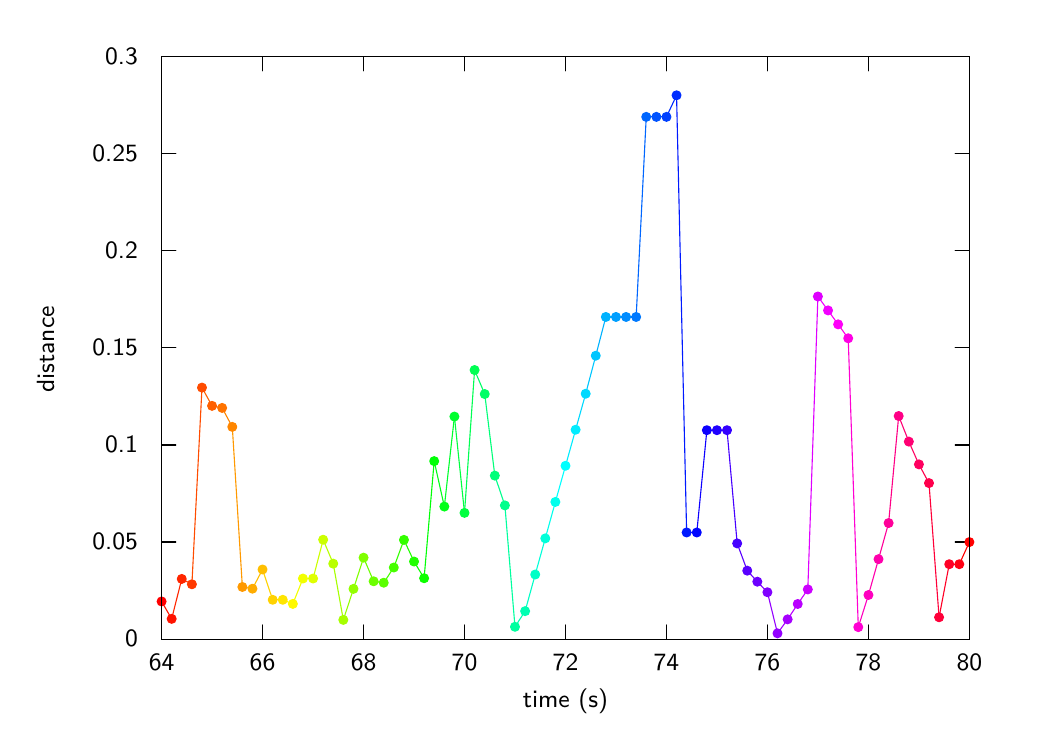
\begin{tikzpicture}[gnuplot]
%% generated with GNUPLOT 4.6p4 (Lua 5.1; terminal rev. 99, script rev. 100)
%% Thu 28 May 2015 09:06:58 AM CEST
\path (0.000,0.000) rectangle (12.500,8.750);
\gpcolor{color=gp lt color border}
\gpsetlinetype{gp lt border}
\gpsetlinewidth{1.00}
\draw[gp path] (1.688,0.985)--(1.868,0.985);
\draw[gp path] (11.947,0.985)--(11.767,0.985);
\node[gp node right,font={\fontsize{9pt}{10.8pt}\selectfont}] at (1.504,0.985) { 0};
\draw[gp path] (1.688,2.218)--(1.868,2.218);
\draw[gp path] (11.947,2.218)--(11.767,2.218);
\node[gp node right,font={\fontsize{9pt}{10.8pt}\selectfont}] at (1.504,2.218) { 0.05};
\draw[gp path] (1.688,3.450)--(1.868,3.450);
\draw[gp path] (11.947,3.450)--(11.767,3.450);
\node[gp node right,font={\fontsize{9pt}{10.8pt}\selectfont}] at (1.504,3.450) { 0.1};
\draw[gp path] (1.688,4.683)--(1.868,4.683);
\draw[gp path] (11.947,4.683)--(11.767,4.683);
\node[gp node right,font={\fontsize{9pt}{10.8pt}\selectfont}] at (1.504,4.683) { 0.15};
\draw[gp path] (1.688,5.916)--(1.868,5.916);
\draw[gp path] (11.947,5.916)--(11.767,5.916);
\node[gp node right,font={\fontsize{9pt}{10.8pt}\selectfont}] at (1.504,5.916) { 0.2};
\draw[gp path] (1.688,7.148)--(1.868,7.148);
\draw[gp path] (11.947,7.148)--(11.767,7.148);
\node[gp node right,font={\fontsize{9pt}{10.8pt}\selectfont}] at (1.504,7.148) { 0.25};
\draw[gp path] (1.688,8.381)--(1.868,8.381);
\draw[gp path] (11.947,8.381)--(11.767,8.381);
\node[gp node right,font={\fontsize{9pt}{10.8pt}\selectfont}] at (1.504,8.381) { 0.3};
\draw[gp path] (1.688,0.985)--(1.688,1.165);
\draw[gp path] (1.688,8.381)--(1.688,8.201);
\node[gp node center,font={\fontsize{9pt}{10.8pt}\selectfont}] at (1.688,0.677) { 64};
\draw[gp path] (2.970,0.985)--(2.970,1.165);
\draw[gp path] (2.970,8.381)--(2.970,8.201);
\node[gp node center,font={\fontsize{9pt}{10.8pt}\selectfont}] at (2.970,0.677) { 66};
\draw[gp path] (4.253,0.985)--(4.253,1.165);
\draw[gp path] (4.253,8.381)--(4.253,8.201);
\node[gp node center,font={\fontsize{9pt}{10.8pt}\selectfont}] at (4.253,0.677) { 68};
\draw[gp path] (5.535,0.985)--(5.535,1.165);
\draw[gp path] (5.535,8.381)--(5.535,8.201);
\node[gp node center,font={\fontsize{9pt}{10.8pt}\selectfont}] at (5.535,0.677) { 70};
\draw[gp path] (6.818,0.985)--(6.818,1.165);
\draw[gp path] (6.818,8.381)--(6.818,8.201);
\node[gp node center,font={\fontsize{9pt}{10.8pt}\selectfont}] at (6.818,0.677) { 72};
\draw[gp path] (8.100,0.985)--(8.100,1.165);
\draw[gp path] (8.100,8.381)--(8.100,8.201);
\node[gp node center,font={\fontsize{9pt}{10.8pt}\selectfont}] at (8.100,0.677) { 74};
\draw[gp path] (9.382,0.985)--(9.382,1.165);
\draw[gp path] (9.382,8.381)--(9.382,8.201);
\node[gp node center,font={\fontsize{9pt}{10.8pt}\selectfont}] at (9.382,0.677) { 76};
\draw[gp path] (10.665,0.985)--(10.665,1.165);
\draw[gp path] (10.665,8.381)--(10.665,8.201);
\node[gp node center,font={\fontsize{9pt}{10.8pt}\selectfont}] at (10.665,0.677) { 78};
\draw[gp path] (11.947,0.985)--(11.947,1.165);
\draw[gp path] (11.947,8.381)--(11.947,8.201);
\node[gp node center,font={\fontsize{9pt}{10.8pt}\selectfont}] at (11.947,0.677) { 80};
\draw[gp path] (1.688,8.381)--(1.688,0.985)--(11.947,0.985)--(11.947,8.381)--cycle;
\node[gp node center,rotate=-270,font={\fontsize{9pt}{10.8pt}\selectfont}] at (0.246,4.683) {distance};
\node[gp node center,font={\fontsize{9pt}{10.8pt}\selectfont}] at (6.817,0.215) {time (s)};
\gpcolor{rgb color={1.000,0.075,0.000}}
\gpsetlinetype{gp lt plot 0}
\draw[gp path] (1.688,1.463)--(1.816,1.242);
\gpcolor{rgb color={1.000,0.150,0.000}}
\draw[gp path] (1.816,1.242)--(1.944,1.749);
\gpcolor{rgb color={1.000,0.225,0.000}}
\draw[gp path] (1.944,1.749)--(2.073,1.681);
\gpcolor{rgb color={1.000,0.300,0.000}}
\draw[gp path] (2.073,1.681)--(2.201,4.179);
\gpcolor{rgb color={1.000,0.375,0.000}}
\draw[gp path] (2.201,4.179)--(2.329,3.947);
\gpcolor{rgb color={1.000,0.450,0.000}}
\draw[gp path] (2.329,3.947)--(2.457,3.921);
\gpcolor{rgb color={1.000,0.525,0.000}}
\draw[gp path] (2.457,3.921)--(2.586,3.680);
\gpcolor{rgb color={1.000,0.600,0.000}}
\draw[gp path] (2.586,3.680)--(2.714,1.647);
\gpcolor{rgb color={1.000,0.675,0.000}}
\draw[gp path] (2.714,1.647)--(2.842,1.625);
\gpcolor{rgb color={1.000,0.750,0.000}}
\draw[gp path] (2.842,1.625)--(2.970,1.869);
\gpcolor{rgb color={1.000,0.825,0.000}}
\draw[gp path] (2.970,1.869)--(3.099,1.484);
\gpcolor{rgb color={1.000,0.900,0.000}}
\draw[gp path] (3.099,1.484)--(3.227,1.484);
\gpcolor{rgb color={1.000,0.975,0.000}}
\draw[gp path] (3.227,1.484)--(3.355,1.432);
\gpcolor{rgb color={0.950,1.000,0.000}}
\draw[gp path] (3.355,1.432)--(3.483,1.754);
\gpcolor{rgb color={0.875,1.000,0.000}}
\draw[gp path] (3.483,1.754)--(3.612,1.754);
\gpcolor{rgb color={0.800,1.000,0.000}}
\draw[gp path] (3.612,1.754)--(3.740,2.247);
\gpcolor{rgb color={0.725,1.000,0.000}}
\draw[gp path] (3.740,2.247)--(3.868,1.943);
\gpcolor{rgb color={0.650,1.000,0.000}}
\draw[gp path] (3.868,1.943)--(3.996,1.229);
\gpcolor{rgb color={0.575,1.000,0.000}}
\draw[gp path] (3.996,1.229)--(4.125,1.623);
\gpcolor{rgb color={0.500,1.000,0.000}}
\draw[gp path] (4.125,1.623)--(4.253,2.019);
\gpcolor{rgb color={0.425,1.000,0.000}}
\draw[gp path] (4.253,2.019)--(4.381,1.719);
\gpcolor{rgb color={0.350,1.000,0.000}}
\draw[gp path] (4.381,1.719)--(4.509,1.701);
\gpcolor{rgb color={0.275,1.000,0.000}}
\draw[gp path] (4.509,1.701)--(4.637,1.894);
\gpcolor{rgb color={0.200,1.000,0.000}}
\draw[gp path] (4.637,1.894)--(4.766,2.245);
\gpcolor{rgb color={0.125,1.000,0.000}}
\draw[gp path] (4.766,2.245)--(4.894,1.970);
\gpcolor{rgb color={0.050,1.000,0.000}}
\draw[gp path] (4.894,1.970)--(5.022,1.758);
\gpcolor{rgb color={0.000,1.000,0.025}}
\draw[gp path] (5.022,1.758)--(5.150,3.245);
\gpcolor{rgb color={0.000,1.000,0.100}}
\draw[gp path] (5.150,3.245)--(5.279,2.668);
\gpcolor{rgb color={0.000,1.000,0.175}}
\draw[gp path] (5.279,2.668)--(5.407,3.811);
\gpcolor{rgb color={0.000,1.000,0.250}}
\draw[gp path] (5.407,3.811)--(5.535,2.588);
\gpcolor{rgb color={0.000,1.000,0.325}}
\draw[gp path] (5.535,2.588)--(5.663,4.402);
\gpcolor{rgb color={0.000,1.000,0.400}}
\draw[gp path] (5.663,4.402)--(5.792,4.097);
\gpcolor{rgb color={0.000,1.000,0.475}}
\draw[gp path] (5.792,4.097)--(5.920,3.061);
\gpcolor{rgb color={0.000,1.000,0.550}}
\draw[gp path] (5.920,3.061)--(6.048,2.683);
\gpcolor{rgb color={0.000,1.000,0.625}}
\draw[gp path] (6.048,2.683)--(6.176,1.141);
\gpcolor{rgb color={0.000,1.000,0.700}}
\draw[gp path] (6.176,1.141)--(6.305,1.340);
\gpcolor{rgb color={0.000,1.000,0.775}}
\draw[gp path] (6.305,1.340)--(6.433,1.805);
\gpcolor{rgb color={0.000,1.000,0.850}}
\draw[gp path] (6.433,1.805)--(6.561,2.264);
\gpcolor{rgb color={0.000,1.000,0.925}}
\draw[gp path] (6.561,2.264)--(6.689,2.727);
\gpcolor{rgb color={0.000,1.000,1.000}}
\draw[gp path] (6.689,2.727)--(6.818,3.186);
\gpcolor{rgb color={0.000,0.925,1.000}}
\draw[gp path] (6.818,3.186)--(6.946,3.644);
\gpcolor{rgb color={0.000,0.850,1.000}}
\draw[gp path] (6.946,3.644)--(7.074,4.101);
\gpcolor{rgb color={0.000,0.775,1.000}}
\draw[gp path] (7.074,4.101)--(7.202,4.584);
\gpcolor{rgb color={0.000,0.700,1.000}}
\draw[gp path] (7.202,4.584)--(7.330,5.076);
\gpcolor{rgb color={0.000,0.625,1.000}}
\draw[gp path] (7.330,5.076)--(7.459,5.076);
\gpcolor{rgb color={0.000,0.550,1.000}}
\draw[gp path] (7.459,5.076)--(7.587,5.076);
\gpcolor{rgb color={0.000,0.475,1.000}}
\draw[gp path] (7.587,5.076)--(7.715,5.076);
\gpcolor{rgb color={0.000,0.400,1.000}}
\draw[gp path] (7.715,5.076)--(7.843,7.617);
\gpcolor{rgb color={0.000,0.325,1.000}}
\draw[gp path] (7.843,7.617)--(7.972,7.617);
\gpcolor{rgb color={0.000,0.250,1.000}}
\draw[gp path] (7.972,7.617)--(8.100,7.617);
\gpcolor{rgb color={0.000,0.175,1.000}}
\draw[gp path] (8.100,7.617)--(8.228,7.891);
\gpcolor{rgb color={0.000,0.100,1.000}}
\draw[gp path] (8.228,7.891)--(8.356,2.339);
\gpcolor{rgb color={0.000,0.025,1.000}}
\draw[gp path] (8.356,2.339)--(8.485,2.339);
\gpcolor{rgb color={0.050,0.000,1.000}}
\draw[gp path] (8.485,2.339)--(8.613,3.638);
\gpcolor{rgb color={0.125,0.000,1.000}}
\draw[gp path] (8.613,3.638)--(8.741,3.638);
\gpcolor{rgb color={0.200,0.000,1.000}}
\draw[gp path] (8.741,3.638)--(8.869,3.638);
\gpcolor{rgb color={0.275,0.000,1.000}}
\draw[gp path] (8.869,3.638)--(8.998,2.200);
\gpcolor{rgb color={0.350,0.000,1.000}}
\draw[gp path] (8.998,2.200)--(9.126,1.854);
\gpcolor{rgb color={0.425,0.000,1.000}}
\draw[gp path] (9.126,1.854)--(9.254,1.714);
\gpcolor{rgb color={0.500,0.000,1.000}}
\draw[gp path] (9.254,1.714)--(9.382,1.580);
\gpcolor{rgb color={0.575,0.000,1.000}}
\draw[gp path] (9.382,1.580)--(9.510,1.058);
\gpcolor{rgb color={0.650,0.000,1.000}}
\draw[gp path] (9.510,1.058)--(9.639,1.236);
\gpcolor{rgb color={0.725,0.000,1.000}}
\draw[gp path] (9.639,1.236)--(9.767,1.431);
\gpcolor{rgb color={0.800,0.000,1.000}}
\draw[gp path] (9.767,1.431)--(9.895,1.616);
\gpcolor{rgb color={0.875,0.000,1.000}}
\draw[gp path] (9.895,1.616)--(10.023,5.336);
\gpcolor{rgb color={0.950,0.000,1.000}}
\draw[gp path] (10.023,5.336)--(10.152,5.159);
\gpcolor{rgb color={1.000,0.000,0.975}}
\draw[gp path] (10.152,5.159)--(10.280,4.982);
\gpcolor{rgb color={1.000,0.000,0.900}}
\draw[gp path] (10.280,4.982)--(10.408,4.805);
\gpcolor{rgb color={1.000,0.000,0.825}}
\draw[gp path] (10.408,4.805)--(10.536,1.137);
\gpcolor{rgb color={1.000,0.000,0.750}}
\draw[gp path] (10.536,1.137)--(10.665,1.545);
\gpcolor{rgb color={1.000,0.000,0.675}}
\draw[gp path] (10.665,1.545)--(10.793,2.000);
\gpcolor{rgb color={1.000,0.000,0.600}}
\draw[gp path] (10.793,2.000)--(10.921,2.459);
\gpcolor{rgb color={1.000,0.000,0.525}}
\draw[gp path] (10.921,2.459)--(11.049,3.818);
\gpcolor{rgb color={1.000,0.000,0.450}}
\draw[gp path] (11.049,3.818)--(11.178,3.493);
\gpcolor{rgb color={1.000,0.000,0.375}}
\draw[gp path] (11.178,3.493)--(11.306,3.204);
\gpcolor{rgb color={1.000,0.000,0.300}}
\draw[gp path] (11.306,3.204)--(11.434,2.966);
\gpcolor{rgb color={1.000,0.000,0.225}}
\draw[gp path] (11.434,2.966)--(11.562,1.262);
\gpcolor{rgb color={1.000,0.000,0.150}}
\draw[gp path] (11.562,1.262)--(11.691,1.936);
\gpcolor{rgb color={1.000,0.000,0.075}}
\draw[gp path] (11.691,1.936)--(11.819,1.936);
\gpcolor{rgb color={1.000,0.000,0.000}}
\draw[gp path] (11.819,1.936)--(11.947,2.217);
\gpsetpointsize{4.00}
\gppoint{gp mark 7}{(1.688,1.463)}
\gpcolor{rgb color={1.000,0.075,0.000}}
\gppoint{gp mark 7}{(1.816,1.242)}
\gpcolor{rgb color={1.000,0.150,0.000}}
\gppoint{gp mark 7}{(1.944,1.749)}
\gpcolor{rgb color={1.000,0.225,0.000}}
\gppoint{gp mark 7}{(2.073,1.681)}
\gpcolor{rgb color={1.000,0.300,0.000}}
\gppoint{gp mark 7}{(2.201,4.179)}
\gpcolor{rgb color={1.000,0.375,0.000}}
\gppoint{gp mark 7}{(2.329,3.947)}
\gpcolor{rgb color={1.000,0.450,0.000}}
\gppoint{gp mark 7}{(2.457,3.921)}
\gpcolor{rgb color={1.000,0.525,0.000}}
\gppoint{gp mark 7}{(2.586,3.680)}
\gpcolor{rgb color={1.000,0.600,0.000}}
\gppoint{gp mark 7}{(2.714,1.647)}
\gpcolor{rgb color={1.000,0.675,0.000}}
\gppoint{gp mark 7}{(2.842,1.625)}
\gpcolor{rgb color={1.000,0.750,0.000}}
\gppoint{gp mark 7}{(2.970,1.869)}
\gpcolor{rgb color={1.000,0.825,0.000}}
\gppoint{gp mark 7}{(3.099,1.484)}
\gpcolor{rgb color={1.000,0.900,0.000}}
\gppoint{gp mark 7}{(3.227,1.484)}
\gpcolor{rgb color={1.000,0.975,0.000}}
\gppoint{gp mark 7}{(3.355,1.432)}
\gpcolor{rgb color={0.950,1.000,0.000}}
\gppoint{gp mark 7}{(3.483,1.754)}
\gpcolor{rgb color={0.875,1.000,0.000}}
\gppoint{gp mark 7}{(3.612,1.754)}
\gpcolor{rgb color={0.800,1.000,0.000}}
\gppoint{gp mark 7}{(3.740,2.247)}
\gpcolor{rgb color={0.725,1.000,0.000}}
\gppoint{gp mark 7}{(3.868,1.943)}
\gpcolor{rgb color={0.650,1.000,0.000}}
\gppoint{gp mark 7}{(3.996,1.229)}
\gpcolor{rgb color={0.575,1.000,0.000}}
\gppoint{gp mark 7}{(4.125,1.623)}
\gpcolor{rgb color={0.500,1.000,0.000}}
\gppoint{gp mark 7}{(4.253,2.019)}
\gpcolor{rgb color={0.425,1.000,0.000}}
\gppoint{gp mark 7}{(4.381,1.719)}
\gpcolor{rgb color={0.350,1.000,0.000}}
\gppoint{gp mark 7}{(4.509,1.701)}
\gpcolor{rgb color={0.275,1.000,0.000}}
\gppoint{gp mark 7}{(4.637,1.894)}
\gpcolor{rgb color={0.200,1.000,0.000}}
\gppoint{gp mark 7}{(4.766,2.245)}
\gpcolor{rgb color={0.125,1.000,0.000}}
\gppoint{gp mark 7}{(4.894,1.970)}
\gpcolor{rgb color={0.050,1.000,0.000}}
\gppoint{gp mark 7}{(5.022,1.758)}
\gpcolor{rgb color={0.000,1.000,0.025}}
\gppoint{gp mark 7}{(5.150,3.245)}
\gpcolor{rgb color={0.000,1.000,0.100}}
\gppoint{gp mark 7}{(5.279,2.668)}
\gpcolor{rgb color={0.000,1.000,0.175}}
\gppoint{gp mark 7}{(5.407,3.811)}
\gpcolor{rgb color={0.000,1.000,0.250}}
\gppoint{gp mark 7}{(5.535,2.588)}
\gpcolor{rgb color={0.000,1.000,0.325}}
\gppoint{gp mark 7}{(5.663,4.402)}
\gpcolor{rgb color={0.000,1.000,0.400}}
\gppoint{gp mark 7}{(5.792,4.097)}
\gpcolor{rgb color={0.000,1.000,0.475}}
\gppoint{gp mark 7}{(5.920,3.061)}
\gpcolor{rgb color={0.000,1.000,0.550}}
\gppoint{gp mark 7}{(6.048,2.683)}
\gpcolor{rgb color={0.000,1.000,0.625}}
\gppoint{gp mark 7}{(6.176,1.141)}
\gpcolor{rgb color={0.000,1.000,0.700}}
\gppoint{gp mark 7}{(6.305,1.340)}
\gpcolor{rgb color={0.000,1.000,0.775}}
\gppoint{gp mark 7}{(6.433,1.805)}
\gpcolor{rgb color={0.000,1.000,0.850}}
\gppoint{gp mark 7}{(6.561,2.264)}
\gpcolor{rgb color={0.000,1.000,0.925}}
\gppoint{gp mark 7}{(6.689,2.727)}
\gpcolor{rgb color={0.000,1.000,1.000}}
\gppoint{gp mark 7}{(6.818,3.186)}
\gpcolor{rgb color={0.000,0.925,1.000}}
\gppoint{gp mark 7}{(6.946,3.644)}
\gpcolor{rgb color={0.000,0.850,1.000}}
\gppoint{gp mark 7}{(7.074,4.101)}
\gpcolor{rgb color={0.000,0.775,1.000}}
\gppoint{gp mark 7}{(7.202,4.584)}
\gpcolor{rgb color={0.000,0.700,1.000}}
\gppoint{gp mark 7}{(7.330,5.076)}
\gpcolor{rgb color={0.000,0.625,1.000}}
\gppoint{gp mark 7}{(7.459,5.076)}
\gpcolor{rgb color={0.000,0.550,1.000}}
\gppoint{gp mark 7}{(7.587,5.076)}
\gpcolor{rgb color={0.000,0.475,1.000}}
\gppoint{gp mark 7}{(7.715,5.076)}
\gpcolor{rgb color={0.000,0.400,1.000}}
\gppoint{gp mark 7}{(7.843,7.617)}
\gpcolor{rgb color={0.000,0.325,1.000}}
\gppoint{gp mark 7}{(7.972,7.617)}
\gpcolor{rgb color={0.000,0.250,1.000}}
\gppoint{gp mark 7}{(8.100,7.617)}
\gpcolor{rgb color={0.000,0.175,1.000}}
\gppoint{gp mark 7}{(8.228,7.891)}
\gpcolor{rgb color={0.000,0.100,1.000}}
\gppoint{gp mark 7}{(8.356,2.339)}
\gpcolor{rgb color={0.000,0.025,1.000}}
\gppoint{gp mark 7}{(8.485,2.339)}
\gpcolor{rgb color={0.050,0.000,1.000}}
\gppoint{gp mark 7}{(8.613,3.638)}
\gpcolor{rgb color={0.125,0.000,1.000}}
\gppoint{gp mark 7}{(8.741,3.638)}
\gpcolor{rgb color={0.200,0.000,1.000}}
\gppoint{gp mark 7}{(8.869,3.638)}
\gpcolor{rgb color={0.275,0.000,1.000}}
\gppoint{gp mark 7}{(8.998,2.200)}
\gpcolor{rgb color={0.350,0.000,1.000}}
\gppoint{gp mark 7}{(9.126,1.854)}
\gpcolor{rgb color={0.425,0.000,1.000}}
\gppoint{gp mark 7}{(9.254,1.714)}
\gpcolor{rgb color={0.500,0.000,1.000}}
\gppoint{gp mark 7}{(9.382,1.580)}
\gpcolor{rgb color={0.575,0.000,1.000}}
\gppoint{gp mark 7}{(9.510,1.058)}
\gpcolor{rgb color={0.650,0.000,1.000}}
\gppoint{gp mark 7}{(9.639,1.236)}
\gpcolor{rgb color={0.725,0.000,1.000}}
\gppoint{gp mark 7}{(9.767,1.431)}
\gpcolor{rgb color={0.800,0.000,1.000}}
\gppoint{gp mark 7}{(9.895,1.616)}
\gpcolor{rgb color={0.875,0.000,1.000}}
\gppoint{gp mark 7}{(10.023,5.336)}
\gpcolor{rgb color={0.950,0.000,1.000}}
\gppoint{gp mark 7}{(10.152,5.159)}
\gpcolor{rgb color={1.000,0.000,0.975}}
\gppoint{gp mark 7}{(10.280,4.982)}
\gpcolor{rgb color={1.000,0.000,0.900}}
\gppoint{gp mark 7}{(10.408,4.805)}
\gpcolor{rgb color={1.000,0.000,0.825}}
\gppoint{gp mark 7}{(10.536,1.137)}
\gpcolor{rgb color={1.000,0.000,0.750}}
\gppoint{gp mark 7}{(10.665,1.545)}
\gpcolor{rgb color={1.000,0.000,0.675}}
\gppoint{gp mark 7}{(10.793,2.000)}
\gpcolor{rgb color={1.000,0.000,0.600}}
\gppoint{gp mark 7}{(10.921,2.459)}
\gpcolor{rgb color={1.000,0.000,0.525}}
\gppoint{gp mark 7}{(11.049,3.818)}
\gpcolor{rgb color={1.000,0.000,0.450}}
\gppoint{gp mark 7}{(11.178,3.493)}
\gpcolor{rgb color={1.000,0.000,0.375}}
\gppoint{gp mark 7}{(11.306,3.204)}
\gpcolor{rgb color={1.000,0.000,0.300}}
\gppoint{gp mark 7}{(11.434,2.966)}
\gpcolor{rgb color={1.000,0.000,0.225}}
\gppoint{gp mark 7}{(11.562,1.262)}
\gpcolor{rgb color={1.000,0.000,0.150}}
\gppoint{gp mark 7}{(11.691,1.936)}
\gpcolor{rgb color={1.000,0.000,0.075}}
\gppoint{gp mark 7}{(11.819,1.936)}
\gpcolor{rgb color={1.000,0.000,0.000}}
\gppoint{gp mark 7}{(11.947,2.217)}
\gpcolor{color=gp lt color border}
\gpsetlinetype{gp lt border}
\draw[gp path] (1.688,8.381)--(1.688,0.985)--(11.947,0.985)--(11.947,8.381)--cycle;
%% coordinates of the plot area
\gpdefrectangularnode{gp plot 1}{\pgfpoint{1.688cm}{0.985cm}}{\pgfpoint{11.947cm}{8.381cm}}
\end{tikzpicture}
%% gnuplot variables

%     }
%     \caption{Err.}
%     \label{fig:ball_kalman_error_tikz}
% \end{figure}

% \begin{figure}[htb]
%     \centering
%     \begin{subfigure}[b]{0.49\textwidth}
%         \resizebox{\columnwidth}{!}{%
%             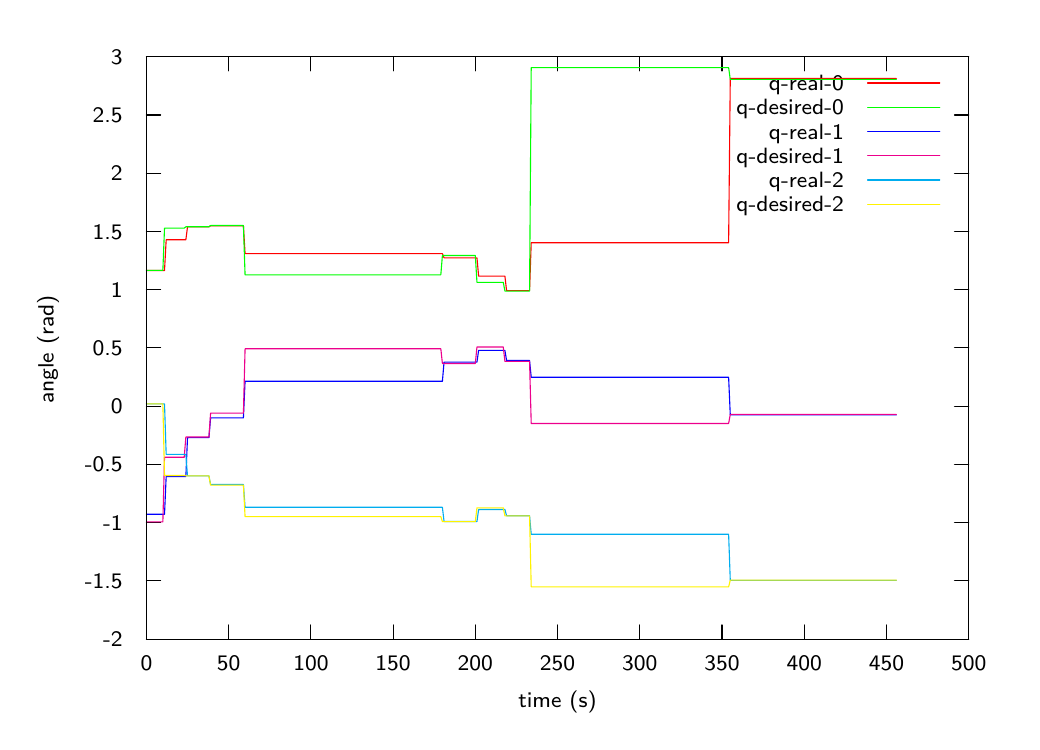
\begin{tikzpicture}[gnuplot]
%% generated with GNUPLOT 4.6p4 (Lua 5.1; terminal rev. 99, script rev. 100)
%% Thu 28 May 2015 12:34:40 AM CEST
\path (0.000,0.000) rectangle (12.500,8.750);
\gpcolor{color=gp lt color border}
\gpsetlinetype{gp lt border}
\gpsetlinewidth{1.00}
\draw[gp path] (1.504,0.985)--(1.684,0.985);
\draw[gp path] (11.947,0.985)--(11.767,0.985);
\node[gp node right,font={\fontsize{8pt}{9.6pt}\selectfont}] at (1.320,0.985) {-2};
\draw[gp path] (1.504,1.725)--(1.684,1.725);
\draw[gp path] (11.947,1.725)--(11.767,1.725);
\node[gp node right,font={\fontsize{8pt}{9.6pt}\selectfont}] at (1.320,1.725) {-1.5};
\draw[gp path] (1.504,2.464)--(1.684,2.464);
\draw[gp path] (11.947,2.464)--(11.767,2.464);
\node[gp node right,font={\fontsize{8pt}{9.6pt}\selectfont}] at (1.320,2.464) {-1};
\draw[gp path] (1.504,3.204)--(1.684,3.204);
\draw[gp path] (11.947,3.204)--(11.767,3.204);
\node[gp node right,font={\fontsize{8pt}{9.6pt}\selectfont}] at (1.320,3.204) {-0.5};
\draw[gp path] (1.504,3.943)--(1.684,3.943);
\draw[gp path] (11.947,3.943)--(11.767,3.943);
\node[gp node right,font={\fontsize{8pt}{9.6pt}\selectfont}] at (1.320,3.943) { 0};
\draw[gp path] (1.504,4.683)--(1.684,4.683);
\draw[gp path] (11.947,4.683)--(11.767,4.683);
\node[gp node right,font={\fontsize{8pt}{9.6pt}\selectfont}] at (1.320,4.683) { 0.5};
\draw[gp path] (1.504,5.423)--(1.684,5.423);
\draw[gp path] (11.947,5.423)--(11.767,5.423);
\node[gp node right,font={\fontsize{8pt}{9.6pt}\selectfont}] at (1.320,5.423) { 1};
\draw[gp path] (1.504,6.162)--(1.684,6.162);
\draw[gp path] (11.947,6.162)--(11.767,6.162);
\node[gp node right,font={\fontsize{8pt}{9.6pt}\selectfont}] at (1.320,6.162) { 1.5};
\draw[gp path] (1.504,6.902)--(1.684,6.902);
\draw[gp path] (11.947,6.902)--(11.767,6.902);
\node[gp node right,font={\fontsize{8pt}{9.6pt}\selectfont}] at (1.320,6.902) { 2};
\draw[gp path] (1.504,7.641)--(1.684,7.641);
\draw[gp path] (11.947,7.641)--(11.767,7.641);
\node[gp node right,font={\fontsize{8pt}{9.6pt}\selectfont}] at (1.320,7.641) { 2.5};
\draw[gp path] (1.504,8.381)--(1.684,8.381);
\draw[gp path] (11.947,8.381)--(11.767,8.381);
\node[gp node right,font={\fontsize{8pt}{9.6pt}\selectfont}] at (1.320,8.381) { 3};
\draw[gp path] (1.504,0.985)--(1.504,1.165);
\draw[gp path] (1.504,8.381)--(1.504,8.201);
\node[gp node center,font={\fontsize{8pt}{9.6pt}\selectfont}] at (1.504,0.677) { 0};
\draw[gp path] (2.548,0.985)--(2.548,1.165);
\draw[gp path] (2.548,8.381)--(2.548,8.201);
\node[gp node center,font={\fontsize{8pt}{9.6pt}\selectfont}] at (2.548,0.677) { 50};
\draw[gp path] (3.593,0.985)--(3.593,1.165);
\draw[gp path] (3.593,8.381)--(3.593,8.201);
\node[gp node center,font={\fontsize{8pt}{9.6pt}\selectfont}] at (3.593,0.677) { 100};
\draw[gp path] (4.637,0.985)--(4.637,1.165);
\draw[gp path] (4.637,8.381)--(4.637,8.201);
\node[gp node center,font={\fontsize{8pt}{9.6pt}\selectfont}] at (4.637,0.677) { 150};
\draw[gp path] (5.681,0.985)--(5.681,1.165);
\draw[gp path] (5.681,8.381)--(5.681,8.201);
\node[gp node center,font={\fontsize{8pt}{9.6pt}\selectfont}] at (5.681,0.677) { 200};
\draw[gp path] (6.726,0.985)--(6.726,1.165);
\draw[gp path] (6.726,8.381)--(6.726,8.201);
\node[gp node center,font={\fontsize{8pt}{9.6pt}\selectfont}] at (6.726,0.677) { 250};
\draw[gp path] (7.770,0.985)--(7.770,1.165);
\draw[gp path] (7.770,8.381)--(7.770,8.201);
\node[gp node center,font={\fontsize{8pt}{9.6pt}\selectfont}] at (7.770,0.677) { 300};
\draw[gp path] (8.814,0.985)--(8.814,1.165);
\draw[gp path] (8.814,8.381)--(8.814,8.201);
\node[gp node center,font={\fontsize{8pt}{9.6pt}\selectfont}] at (8.814,0.677) { 350};
\draw[gp path] (9.858,0.985)--(9.858,1.165);
\draw[gp path] (9.858,8.381)--(9.858,8.201);
\node[gp node center,font={\fontsize{8pt}{9.6pt}\selectfont}] at (9.858,0.677) { 400};
\draw[gp path] (10.903,0.985)--(10.903,1.165);
\draw[gp path] (10.903,8.381)--(10.903,8.201);
\node[gp node center,font={\fontsize{8pt}{9.6pt}\selectfont}] at (10.903,0.677) { 450};
\draw[gp path] (11.947,0.985)--(11.947,1.165);
\draw[gp path] (11.947,8.381)--(11.947,8.201);
\node[gp node center,font={\fontsize{8pt}{9.6pt}\selectfont}] at (11.947,0.677) { 500};
\draw[gp path] (1.504,8.381)--(1.504,0.985)--(11.947,0.985)--(11.947,8.381)--cycle;
\node[gp node center,rotate=-270,font={\fontsize{8pt}{9.6pt}\selectfont}] at (0.246,4.683) {angle (rad)};
\node[gp node center,font={\fontsize{8pt}{9.6pt}\selectfont}] at (6.725,0.215) {time (s)};
\node[gp node right,font={\fontsize{8pt}{9.6pt}\selectfont}] at (10.479,8.047) {q-real-0};
\gpcolor{color=gp lt color 0}
\gpsetlinetype{gp lt plot 0}
\draw[gp path] (10.663,8.047)--(11.579,8.047);
\draw[gp path] (1.504,5.666)--(1.525,5.666)--(1.546,5.666)--(1.567,5.666)--(1.588,5.666)%
  --(1.608,5.666)--(1.629,5.666)--(1.650,5.666)--(1.671,5.666)--(1.692,5.666)--(1.713,5.666)%
  --(1.734,5.666)--(1.755,6.056)--(1.776,6.056)--(1.796,6.056)--(1.817,6.056)--(1.838,6.056)%
  --(1.859,6.056)--(1.880,6.056)--(1.901,6.056)--(1.922,6.056)--(1.943,6.056)--(1.963,6.056)%
  --(1.984,6.056)--(2.005,6.056)--(2.026,6.220)--(2.047,6.220)--(2.068,6.220)--(2.089,6.220)%
  --(2.110,6.220)--(2.131,6.220)--(2.151,6.220)--(2.172,6.220)--(2.193,6.220)--(2.214,6.220)%
  --(2.235,6.220)--(2.256,6.220)--(2.277,6.220)--(2.298,6.220)--(2.319,6.235)--(2.339,6.235)%
  --(2.360,6.235)--(2.381,6.235)--(2.402,6.235)--(2.423,6.235)--(2.444,6.235)--(2.465,6.235)%
  --(2.486,6.235)--(2.507,6.235)--(2.527,6.235)--(2.548,6.235)--(2.569,6.235)--(2.590,6.235)%
  --(2.611,6.235)--(2.632,6.235)--(2.653,6.235)--(2.674,6.235)--(2.695,6.235)--(2.715,6.235)%
  --(2.736,6.235)--(2.757,5.881)--(2.778,5.881)--(2.799,5.881)--(2.820,5.881)--(2.841,5.881)%
  --(2.862,5.881)--(2.882,5.881)--(2.903,5.881)--(2.924,5.881)--(2.945,5.881)--(2.966,5.881)%
  --(2.987,5.881)--(3.008,5.881)--(3.029,5.881)--(3.050,5.881)--(3.070,5.881)--(3.091,5.881)%
  --(3.112,5.881)--(3.133,5.881)--(3.154,5.881)--(3.175,5.881)--(3.196,5.881)--(3.217,5.881)%
  --(3.238,5.881)--(3.258,5.881)--(3.279,5.881)--(3.300,5.881)--(3.321,5.881)--(3.342,5.881)%
  --(3.363,5.881)--(3.384,5.881)--(3.405,5.881)--(3.426,5.881)--(3.446,5.881)--(3.467,5.881)%
  --(3.488,5.881)--(3.509,5.881)--(3.530,5.881)--(3.551,5.881)--(3.572,5.881)--(3.593,5.881)%
  --(3.613,5.881)--(3.634,5.881)--(3.655,5.881)--(3.676,5.881)--(3.697,5.881)--(3.718,5.881)%
  --(3.739,5.881)--(3.760,5.881)--(3.781,5.881)--(3.801,5.881)--(3.822,5.881)--(3.843,5.881)%
  --(3.864,5.881)--(3.885,5.881)--(3.906,5.881)--(3.927,5.881)--(3.948,5.881)--(3.969,5.881)%
  --(3.989,5.881)--(4.010,5.881)--(4.031,5.881)--(4.052,5.881)--(4.073,5.881)--(4.094,5.881)%
  --(4.115,5.881)--(4.136,5.881)--(4.157,5.881)--(4.177,5.881)--(4.198,5.881)--(4.219,5.881)%
  --(4.240,5.881)--(4.261,5.881)--(4.282,5.881)--(4.303,5.881)--(4.324,5.881)--(4.344,5.881)%
  --(4.365,5.881)--(4.386,5.881)--(4.407,5.881)--(4.428,5.881)--(4.449,5.881)--(4.470,5.881)%
  --(4.491,5.881)--(4.512,5.881)--(4.532,5.881)--(4.553,5.881)--(4.574,5.881)--(4.595,5.881)%
  --(4.616,5.881)--(4.637,5.881)--(4.658,5.881)--(4.679,5.881)--(4.700,5.881)--(4.720,5.881)%
  --(4.741,5.881)--(4.762,5.881)--(4.783,5.881)--(4.804,5.881)--(4.825,5.881)--(4.846,5.881)%
  --(4.867,5.881)--(4.888,5.881)--(4.908,5.881)--(4.929,5.881)--(4.950,5.881)--(4.971,5.881)%
  --(4.992,5.881)--(5.013,5.881)--(5.034,5.881)--(5.055,5.881)--(5.076,5.881)--(5.096,5.881)%
  --(5.117,5.881)--(5.138,5.881)--(5.159,5.881)--(5.180,5.881)--(5.201,5.881)--(5.222,5.881)%
  --(5.243,5.881)--(5.263,5.881)--(5.284,5.827)--(5.305,5.827)--(5.326,5.827)--(5.347,5.827)%
  --(5.368,5.827)--(5.389,5.827)--(5.410,5.827)--(5.431,5.827)--(5.451,5.827)--(5.472,5.827)%
  --(5.493,5.827)--(5.514,5.827)--(5.535,5.827)--(5.556,5.827)--(5.577,5.827)--(5.598,5.827)%
  --(5.619,5.827)--(5.639,5.827)--(5.660,5.827)--(5.681,5.827)--(5.702,5.827)--(5.723,5.594)%
  --(5.744,5.594)--(5.765,5.594)--(5.786,5.594)--(5.807,5.594)--(5.827,5.594)--(5.848,5.594)%
  --(5.869,5.594)--(5.890,5.594)--(5.911,5.594)--(5.932,5.594)--(5.953,5.594)--(5.974,5.594)%
  --(5.994,5.594)--(6.015,5.594)--(6.036,5.594)--(6.057,5.594)--(6.078,5.411)--(6.099,5.411)%
  --(6.120,5.411)--(6.141,5.411)--(6.162,5.411)--(6.182,5.411)--(6.203,5.411)--(6.224,5.411)%
  --(6.245,5.411)--(6.266,5.411)--(6.287,5.411)--(6.308,5.411)--(6.329,5.411)--(6.350,5.411)%
  --(6.370,5.411)--(6.391,6.019)--(6.412,6.019)--(6.433,6.019)--(6.454,6.019)--(6.475,6.019)%
  --(6.496,6.019)--(6.517,6.019)--(6.538,6.019)--(6.558,6.019)--(6.579,6.019)--(6.600,6.019)%
  --(6.621,6.019)--(6.642,6.019)--(6.663,6.019)--(6.684,6.019)--(6.705,6.019)--(6.726,6.019)%
  --(6.746,6.019)--(6.767,6.019)--(6.788,6.019)--(6.809,6.019)--(6.830,6.019)--(6.851,6.019)%
  --(6.872,6.019)--(6.893,6.019)--(6.913,6.019)--(6.934,6.019)--(6.955,6.019)--(6.976,6.019)%
  --(6.997,6.019)--(7.018,6.019)--(7.039,6.019)--(7.060,6.019)--(7.081,6.019)--(7.101,6.019)%
  --(7.122,6.019)--(7.143,6.019)--(7.164,6.019)--(7.185,6.019)--(7.206,6.019)--(7.227,6.019)%
  --(7.248,6.019)--(7.269,6.019)--(7.289,6.019)--(7.310,6.019)--(7.331,6.019)--(7.352,6.019)%
  --(7.373,6.019)--(7.394,6.019)--(7.415,6.019)--(7.436,6.019)--(7.457,6.019)--(7.477,6.019)%
  --(7.498,6.019)--(7.519,6.019)--(7.540,6.019)--(7.561,6.019)--(7.582,6.019)--(7.603,6.019)%
  --(7.624,6.019)--(7.644,6.019)--(7.665,6.019)--(7.686,6.019)--(7.707,6.019)--(7.728,6.019)%
  --(7.749,6.019)--(7.770,6.019)--(7.791,6.019)--(7.812,6.019)--(7.832,6.019)--(7.853,6.019)%
  --(7.874,6.019)--(7.895,6.019)--(7.916,6.019)--(7.937,6.019)--(7.958,6.019)--(7.979,6.019)%
  --(8.000,6.019)--(8.020,6.019)--(8.041,6.019)--(8.062,6.019)--(8.083,6.019)--(8.104,6.019)%
  --(8.125,6.019)--(8.146,6.019)--(8.167,6.019)--(8.188,6.019)--(8.208,6.019)--(8.229,6.019)%
  --(8.250,6.019)--(8.271,6.019)--(8.292,6.019)--(8.313,6.019)--(8.334,6.019)--(8.355,6.019)%
  --(8.375,6.019)--(8.396,6.019)--(8.417,6.019)--(8.438,6.019)--(8.459,6.019)--(8.480,6.019)%
  --(8.501,6.019)--(8.522,6.019)--(8.543,6.019)--(8.563,6.019)--(8.584,6.019)--(8.605,6.019)%
  --(8.626,6.019)--(8.647,6.019)--(8.668,6.019)--(8.689,6.019)--(8.710,6.019)--(8.731,6.019)%
  --(8.751,6.019)--(8.772,6.019)--(8.793,6.019)--(8.814,6.019)--(8.835,6.019)--(8.856,6.019)%
  --(8.877,6.019)--(8.898,6.019)--(8.919,8.104)--(8.939,8.104)--(8.960,8.104)--(8.981,8.104)%
  --(9.002,8.104)--(9.023,8.104)--(9.044,8.104)--(9.065,8.104)--(9.086,8.104)--(9.107,8.104)%
  --(9.127,8.104)--(9.148,8.104)--(9.169,8.104)--(9.190,8.104)--(9.211,8.104)--(9.232,8.104)%
  --(9.253,8.104)--(9.274,8.104)--(9.294,8.104)--(9.315,8.104)--(9.336,8.104)--(9.357,8.104)%
  --(9.378,8.104)--(9.399,8.104)--(9.420,8.104)--(9.441,8.104)--(9.462,8.104)--(9.482,8.104)%
  --(9.503,8.104)--(9.524,8.104)--(9.545,8.104)--(9.566,8.104)--(9.587,8.104)--(9.608,8.104)%
  --(9.629,8.104)--(9.650,8.104)--(9.670,8.104)--(9.691,8.104)--(9.712,8.104)--(9.733,8.104)%
  --(9.754,8.104)--(9.775,8.104)--(9.796,8.104)--(9.817,8.104)--(9.838,8.104)--(9.858,8.104)%
  --(9.879,8.104)--(9.900,8.104)--(9.921,8.104)--(9.942,8.104)--(9.963,8.104)--(9.984,8.104)%
  --(10.005,8.104)--(10.025,8.104)--(10.046,8.104)--(10.067,8.104)--(10.088,8.104)--(10.109,8.104)%
  --(10.130,8.104)--(10.151,8.104)--(10.172,8.104)--(10.193,8.104)--(10.213,8.104)--(10.234,8.104)%
  --(10.255,8.104)--(10.276,8.104)--(10.297,8.104)--(10.318,8.104)--(10.339,8.104)--(10.360,8.104)%
  --(10.381,8.104)--(10.401,8.104)--(10.422,8.104)--(10.443,8.104)--(10.464,8.104)--(10.485,8.104)%
  --(10.506,8.104)--(10.527,8.104)--(10.548,8.104)--(10.569,8.104)--(10.589,8.104)--(10.610,8.104)%
  --(10.631,8.104)--(10.652,8.104)--(10.673,8.104)--(10.694,8.104)--(10.715,8.104)--(10.736,8.104)%
  --(10.756,8.104)--(10.777,8.104)--(10.798,8.104)--(10.819,8.104)--(10.840,8.104)--(10.861,8.104)%
  --(10.882,8.104)--(10.903,8.104)--(10.924,8.104)--(10.944,8.104)--(10.965,8.104)--(10.986,8.104)%
  --(11.007,8.104)--(11.028,8.104);
\gpcolor{color=gp lt color border}
\node[gp node right,font={\fontsize{8pt}{9.6pt}\selectfont}] at (10.479,7.739) {q-desired-0};
\gpcolor{color=gp lt color 1}
\gpsetlinetype{gp lt plot 1}
\draw[gp path] (10.663,7.739)--(11.579,7.739);
\draw[gp path] (1.504,5.668)--(1.525,5.668)--(1.546,5.668)--(1.567,5.668)--(1.588,5.668)%
  --(1.608,5.668)--(1.629,5.668)--(1.650,5.668)--(1.671,5.668)--(1.692,5.668)--(1.713,5.668)%
  --(1.734,6.205)--(1.755,6.205)--(1.776,6.205)--(1.796,6.205)--(1.817,6.205)--(1.838,6.205)%
  --(1.859,6.205)--(1.880,6.205)--(1.901,6.205)--(1.922,6.205)--(1.943,6.205)--(1.963,6.205)%
  --(1.984,6.205)--(2.005,6.221)--(2.026,6.221)--(2.047,6.221)--(2.068,6.221)--(2.089,6.221)%
  --(2.110,6.221)--(2.131,6.221)--(2.151,6.221)--(2.172,6.221)--(2.193,6.221)--(2.214,6.221)%
  --(2.235,6.221)--(2.256,6.221)--(2.277,6.221)--(2.298,6.221)--(2.319,6.237)--(2.339,6.237)%
  --(2.360,6.237)--(2.381,6.237)--(2.402,6.237)--(2.423,6.237)--(2.444,6.237)--(2.465,6.237)%
  --(2.486,6.237)--(2.507,6.237)--(2.527,6.237)--(2.548,6.237)--(2.569,6.237)--(2.590,6.237)%
  --(2.611,6.237)--(2.632,6.237)--(2.653,6.237)--(2.674,6.237)--(2.695,6.237)--(2.715,6.237)%
  --(2.736,6.237)--(2.757,5.611)--(2.778,5.611)--(2.799,5.611)--(2.820,5.611)--(2.841,5.611)%
  --(2.862,5.611)--(2.882,5.611)--(2.903,5.611)--(2.924,5.611)--(2.945,5.611)--(2.966,5.611)%
  --(2.987,5.611)--(3.008,5.611)--(3.029,5.611)--(3.050,5.611)--(3.070,5.611)--(3.091,5.611)%
  --(3.112,5.611)--(3.133,5.611)--(3.154,5.611)--(3.175,5.611)--(3.196,5.611)--(3.217,5.611)%
  --(3.238,5.611)--(3.258,5.611)--(3.279,5.611)--(3.300,5.611)--(3.321,5.611)--(3.342,5.611)%
  --(3.363,5.611)--(3.384,5.611)--(3.405,5.611)--(3.426,5.611)--(3.446,5.611)--(3.467,5.611)%
  --(3.488,5.611)--(3.509,5.611)--(3.530,5.611)--(3.551,5.611)--(3.572,5.611)--(3.593,5.611)%
  --(3.613,5.611)--(3.634,5.611)--(3.655,5.611)--(3.676,5.611)--(3.697,5.611)--(3.718,5.611)%
  --(3.739,5.611)--(3.760,5.611)--(3.781,5.611)--(3.801,5.611)--(3.822,5.611)--(3.843,5.611)%
  --(3.864,5.611)--(3.885,5.611)--(3.906,5.611)--(3.927,5.611)--(3.948,5.611)--(3.969,5.611)%
  --(3.989,5.611)--(4.010,5.611)--(4.031,5.611)--(4.052,5.611)--(4.073,5.611)--(4.094,5.611)%
  --(4.115,5.611)--(4.136,5.611)--(4.157,5.611)--(4.177,5.611)--(4.198,5.611)--(4.219,5.611)%
  --(4.240,5.611)--(4.261,5.611)--(4.282,5.611)--(4.303,5.611)--(4.324,5.611)--(4.344,5.611)%
  --(4.365,5.611)--(4.386,5.611)--(4.407,5.611)--(4.428,5.611)--(4.449,5.611)--(4.470,5.611)%
  --(4.491,5.611)--(4.512,5.611)--(4.532,5.611)--(4.553,5.611)--(4.574,5.611)--(4.595,5.611)%
  --(4.616,5.611)--(4.637,5.611)--(4.658,5.611)--(4.679,5.611)--(4.700,5.611)--(4.720,5.611)%
  --(4.741,5.611)--(4.762,5.611)--(4.783,5.611)--(4.804,5.611)--(4.825,5.611)--(4.846,5.611)%
  --(4.867,5.611)--(4.888,5.611)--(4.908,5.611)--(4.929,5.611)--(4.950,5.611)--(4.971,5.611)%
  --(4.992,5.611)--(5.013,5.611)--(5.034,5.611)--(5.055,5.611)--(5.076,5.611)--(5.096,5.611)%
  --(5.117,5.611)--(5.138,5.611)--(5.159,5.611)--(5.180,5.611)--(5.201,5.611)--(5.222,5.611)%
  --(5.243,5.611)--(5.263,5.857)--(5.284,5.857)--(5.305,5.857)--(5.326,5.857)--(5.347,5.857)%
  --(5.368,5.857)--(5.389,5.857)--(5.410,5.857)--(5.431,5.857)--(5.451,5.857)--(5.472,5.857)%
  --(5.493,5.857)--(5.514,5.857)--(5.535,5.857)--(5.556,5.857)--(5.577,5.857)--(5.598,5.857)%
  --(5.619,5.857)--(5.639,5.857)--(5.660,5.857)--(5.681,5.857)--(5.702,5.516)--(5.723,5.516)%
  --(5.744,5.516)--(5.765,5.516)--(5.786,5.516)--(5.807,5.516)--(5.827,5.516)--(5.848,5.516)%
  --(5.869,5.516)--(5.890,5.516)--(5.911,5.516)--(5.932,5.516)--(5.953,5.516)--(5.974,5.516)%
  --(5.994,5.516)--(6.015,5.516)--(6.036,5.516)--(6.057,5.405)--(6.078,5.405)--(6.099,5.405)%
  --(6.120,5.405)--(6.141,5.405)--(6.162,5.405)--(6.182,5.405)--(6.203,5.405)--(6.224,5.405)%
  --(6.245,5.405)--(6.266,5.405)--(6.287,5.405)--(6.308,5.405)--(6.329,5.405)--(6.350,5.405)%
  --(6.370,5.405)--(6.391,8.243)--(6.412,8.243)--(6.433,8.243)--(6.454,8.243)--(6.475,8.243)%
  --(6.496,8.243)--(6.517,8.243)--(6.538,8.243)--(6.558,8.243)--(6.579,8.243)--(6.600,8.243)%
  --(6.621,8.243)--(6.642,8.243)--(6.663,8.243)--(6.684,8.243)--(6.705,8.243)--(6.726,8.243)%
  --(6.746,8.243)--(6.767,8.243)--(6.788,8.243)--(6.809,8.243)--(6.830,8.243)--(6.851,8.243)%
  --(6.872,8.243)--(6.893,8.243)--(6.913,8.243)--(6.934,8.243)--(6.955,8.243)--(6.976,8.243)%
  --(6.997,8.243)--(7.018,8.243)--(7.039,8.243)--(7.060,8.243)--(7.081,8.243)--(7.101,8.243)%
  --(7.122,8.243)--(7.143,8.243)--(7.164,8.243)--(7.185,8.243)--(7.206,8.243)--(7.227,8.243)%
  --(7.248,8.243)--(7.269,8.243)--(7.289,8.243)--(7.310,8.243)--(7.331,8.243)--(7.352,8.243)%
  --(7.373,8.243)--(7.394,8.243)--(7.415,8.243)--(7.436,8.243)--(7.457,8.243)--(7.477,8.243)%
  --(7.498,8.243)--(7.519,8.243)--(7.540,8.243)--(7.561,8.243)--(7.582,8.243)--(7.603,8.243)%
  --(7.624,8.243)--(7.644,8.243)--(7.665,8.243)--(7.686,8.243)--(7.707,8.243)--(7.728,8.243)%
  --(7.749,8.243)--(7.770,8.243)--(7.791,8.243)--(7.812,8.243)--(7.832,8.243)--(7.853,8.243)%
  --(7.874,8.243)--(7.895,8.243)--(7.916,8.243)--(7.937,8.243)--(7.958,8.243)--(7.979,8.243)%
  --(8.000,8.243)--(8.020,8.243)--(8.041,8.243)--(8.062,8.243)--(8.083,8.243)--(8.104,8.243)%
  --(8.125,8.243)--(8.146,8.243)--(8.167,8.243)--(8.188,8.243)--(8.208,8.243)--(8.229,8.243)%
  --(8.250,8.243)--(8.271,8.243)--(8.292,8.243)--(8.313,8.243)--(8.334,8.243)--(8.355,8.243)%
  --(8.375,8.243)--(8.396,8.243)--(8.417,8.243)--(8.438,8.243)--(8.459,8.243)--(8.480,8.243)%
  --(8.501,8.243)--(8.522,8.243)--(8.543,8.243)--(8.563,8.243)--(8.584,8.243)--(8.605,8.243)%
  --(8.626,8.243)--(8.647,8.243)--(8.668,8.243)--(8.689,8.243)--(8.710,8.243)--(8.731,8.243)%
  --(8.751,8.243)--(8.772,8.243)--(8.793,8.243)--(8.814,8.243)--(8.835,8.243)--(8.856,8.243)%
  --(8.877,8.243)--(8.898,8.243)--(8.919,8.093)--(8.939,8.093)--(8.960,8.093)--(8.981,8.093)%
  --(9.002,8.093)--(9.023,8.093)--(9.044,8.093)--(9.065,8.093)--(9.086,8.093)--(9.107,8.093)%
  --(9.127,8.093)--(9.148,8.093)--(9.169,8.093)--(9.190,8.093)--(9.211,8.093)--(9.232,8.093)%
  --(9.253,8.093)--(9.274,8.093)--(9.294,8.093)--(9.315,8.093)--(9.336,8.093)--(9.357,8.093)%
  --(9.378,8.093)--(9.399,8.093)--(9.420,8.093)--(9.441,8.093)--(9.462,8.093)--(9.482,8.093)%
  --(9.503,8.093)--(9.524,8.093)--(9.545,8.093)--(9.566,8.093)--(9.587,8.093)--(9.608,8.093)%
  --(9.629,8.093)--(9.650,8.093)--(9.670,8.093)--(9.691,8.093)--(9.712,8.093)--(9.733,8.093)%
  --(9.754,8.093)--(9.775,8.093)--(9.796,8.093)--(9.817,8.093)--(9.838,8.093)--(9.858,8.093)%
  --(9.879,8.093)--(9.900,8.093)--(9.921,8.093)--(9.942,8.093)--(9.963,8.093)--(9.984,8.093)%
  --(10.005,8.093)--(10.025,8.093)--(10.046,8.093)--(10.067,8.093)--(10.088,8.093)--(10.109,8.093)%
  --(10.130,8.093)--(10.151,8.093)--(10.172,8.093)--(10.193,8.093)--(10.213,8.093)--(10.234,8.093)%
  --(10.255,8.093)--(10.276,8.093)--(10.297,8.093)--(10.318,8.093)--(10.339,8.093)--(10.360,8.093)%
  --(10.381,8.093)--(10.401,8.093)--(10.422,8.093)--(10.443,8.093)--(10.464,8.093)--(10.485,8.093)%
  --(10.506,8.093)--(10.527,8.093)--(10.548,8.093)--(10.569,8.093)--(10.589,8.093)--(10.610,8.093)%
  --(10.631,8.093)--(10.652,8.093)--(10.673,8.093)--(10.694,8.093)--(10.715,8.093)--(10.736,8.093)%
  --(10.756,8.093)--(10.777,8.093)--(10.798,8.093)--(10.819,8.093)--(10.840,8.093)--(10.861,8.093)%
  --(10.882,8.093)--(10.903,8.093)--(10.924,8.093)--(10.944,8.093)--(10.965,8.093)--(10.986,8.093)%
  --(11.007,8.093)--(11.028,8.093);
\gpcolor{color=gp lt color border}
\node[gp node right,font={\fontsize{8pt}{9.6pt}\selectfont}] at (10.479,7.431) {q-real-1};
\gpcolor{color=gp lt color 2}
\gpsetlinetype{gp lt plot 2}
\draw[gp path] (10.663,7.431)--(11.579,7.431);
\draw[gp path] (1.504,2.570)--(1.525,2.570)--(1.546,2.570)--(1.567,2.570)--(1.588,2.570)%
  --(1.608,2.570)--(1.629,2.570)--(1.650,2.570)--(1.671,2.570)--(1.692,2.570)--(1.713,2.570)%
  --(1.734,2.570)--(1.755,3.050)--(1.776,3.050)--(1.796,3.050)--(1.817,3.050)--(1.838,3.050)%
  --(1.859,3.050)--(1.880,3.050)--(1.901,3.050)--(1.922,3.050)--(1.943,3.050)--(1.963,3.050)%
  --(1.984,3.050)--(2.005,3.050)--(2.026,3.543)--(2.047,3.543)--(2.068,3.543)--(2.089,3.543)%
  --(2.110,3.543)--(2.131,3.543)--(2.151,3.543)--(2.172,3.543)--(2.193,3.543)--(2.214,3.543)%
  --(2.235,3.543)--(2.256,3.543)--(2.277,3.543)--(2.298,3.543)--(2.319,3.795)--(2.339,3.795)%
  --(2.360,3.795)--(2.381,3.795)--(2.402,3.795)--(2.423,3.795)--(2.444,3.795)--(2.465,3.795)%
  --(2.486,3.795)--(2.507,3.795)--(2.527,3.795)--(2.548,3.795)--(2.569,3.795)--(2.590,3.795)%
  --(2.611,3.795)--(2.632,3.795)--(2.653,3.795)--(2.674,3.795)--(2.695,3.795)--(2.715,3.795)%
  --(2.736,3.795)--(2.757,4.259)--(2.778,4.259)--(2.799,4.259)--(2.820,4.259)--(2.841,4.259)%
  --(2.862,4.259)--(2.882,4.259)--(2.903,4.259)--(2.924,4.259)--(2.945,4.259)--(2.966,4.259)%
  --(2.987,4.259)--(3.008,4.259)--(3.029,4.259)--(3.050,4.259)--(3.070,4.259)--(3.091,4.259)%
  --(3.112,4.259)--(3.133,4.259)--(3.154,4.259)--(3.175,4.259)--(3.196,4.259)--(3.217,4.259)%
  --(3.238,4.259)--(3.258,4.259)--(3.279,4.259)--(3.300,4.259)--(3.321,4.259)--(3.342,4.259)%
  --(3.363,4.259)--(3.384,4.259)--(3.405,4.259)--(3.426,4.259)--(3.446,4.259)--(3.467,4.259)%
  --(3.488,4.259)--(3.509,4.259)--(3.530,4.259)--(3.551,4.259)--(3.572,4.259)--(3.593,4.259)%
  --(3.613,4.259)--(3.634,4.259)--(3.655,4.259)--(3.676,4.259)--(3.697,4.259)--(3.718,4.259)%
  --(3.739,4.259)--(3.760,4.259)--(3.781,4.259)--(3.801,4.259)--(3.822,4.259)--(3.843,4.259)%
  --(3.864,4.259)--(3.885,4.259)--(3.906,4.259)--(3.927,4.259)--(3.948,4.259)--(3.969,4.259)%
  --(3.989,4.259)--(4.010,4.259)--(4.031,4.259)--(4.052,4.259)--(4.073,4.259)--(4.094,4.259)%
  --(4.115,4.259)--(4.136,4.259)--(4.157,4.259)--(4.177,4.259)--(4.198,4.259)--(4.219,4.259)%
  --(4.240,4.259)--(4.261,4.259)--(4.282,4.259)--(4.303,4.259)--(4.324,4.259)--(4.344,4.259)%
  --(4.365,4.259)--(4.386,4.259)--(4.407,4.259)--(4.428,4.259)--(4.449,4.259)--(4.470,4.259)%
  --(4.491,4.259)--(4.512,4.259)--(4.532,4.259)--(4.553,4.259)--(4.574,4.259)--(4.595,4.259)%
  --(4.616,4.259)--(4.637,4.259)--(4.658,4.259)--(4.679,4.259)--(4.700,4.259)--(4.720,4.259)%
  --(4.741,4.259)--(4.762,4.259)--(4.783,4.259)--(4.804,4.259)--(4.825,4.259)--(4.846,4.259)%
  --(4.867,4.259)--(4.888,4.259)--(4.908,4.259)--(4.929,4.259)--(4.950,4.259)--(4.971,4.259)%
  --(4.992,4.259)--(5.013,4.259)--(5.034,4.259)--(5.055,4.259)--(5.076,4.259)--(5.096,4.259)%
  --(5.117,4.259)--(5.138,4.259)--(5.159,4.259)--(5.180,4.259)--(5.201,4.259)--(5.222,4.259)%
  --(5.243,4.259)--(5.263,4.259)--(5.284,4.503)--(5.305,4.503)--(5.326,4.503)--(5.347,4.503)%
  --(5.368,4.503)--(5.389,4.503)--(5.410,4.503)--(5.431,4.503)--(5.451,4.503)--(5.472,4.503)%
  --(5.493,4.503)--(5.514,4.503)--(5.535,4.503)--(5.556,4.503)--(5.577,4.503)--(5.598,4.503)%
  --(5.619,4.503)--(5.639,4.503)--(5.660,4.503)--(5.681,4.503)--(5.702,4.503)--(5.723,4.651)%
  --(5.744,4.651)--(5.765,4.651)--(5.786,4.651)--(5.807,4.651)--(5.827,4.651)--(5.848,4.651)%
  --(5.869,4.651)--(5.890,4.651)--(5.911,4.651)--(5.932,4.651)--(5.953,4.651)--(5.974,4.651)%
  --(5.994,4.651)--(6.015,4.651)--(6.036,4.651)--(6.057,4.651)--(6.078,4.523)--(6.099,4.523)%
  --(6.120,4.523)--(6.141,4.523)--(6.162,4.523)--(6.182,4.523)--(6.203,4.523)--(6.224,4.523)%
  --(6.245,4.523)--(6.266,4.523)--(6.287,4.523)--(6.308,4.523)--(6.329,4.523)--(6.350,4.523)%
  --(6.370,4.523)--(6.391,4.311)--(6.412,4.311)--(6.433,4.311)--(6.454,4.311)--(6.475,4.311)%
  --(6.496,4.311)--(6.517,4.311)--(6.538,4.311)--(6.558,4.311)--(6.579,4.311)--(6.600,4.311)%
  --(6.621,4.311)--(6.642,4.311)--(6.663,4.311)--(6.684,4.311)--(6.705,4.311)--(6.726,4.311)%
  --(6.746,4.311)--(6.767,4.311)--(6.788,4.311)--(6.809,4.311)--(6.830,4.311)--(6.851,4.311)%
  --(6.872,4.311)--(6.893,4.311)--(6.913,4.311)--(6.934,4.311)--(6.955,4.311)--(6.976,4.311)%
  --(6.997,4.311)--(7.018,4.311)--(7.039,4.311)--(7.060,4.311)--(7.081,4.311)--(7.101,4.311)%
  --(7.122,4.311)--(7.143,4.311)--(7.164,4.311)--(7.185,4.311)--(7.206,4.311)--(7.227,4.311)%
  --(7.248,4.311)--(7.269,4.311)--(7.289,4.311)--(7.310,4.311)--(7.331,4.311)--(7.352,4.311)%
  --(7.373,4.311)--(7.394,4.311)--(7.415,4.311)--(7.436,4.311)--(7.457,4.311)--(7.477,4.311)%
  --(7.498,4.311)--(7.519,4.311)--(7.540,4.311)--(7.561,4.311)--(7.582,4.311)--(7.603,4.311)%
  --(7.624,4.311)--(7.644,4.311)--(7.665,4.311)--(7.686,4.311)--(7.707,4.311)--(7.728,4.311)%
  --(7.749,4.311)--(7.770,4.311)--(7.791,4.311)--(7.812,4.311)--(7.832,4.311)--(7.853,4.311)%
  --(7.874,4.311)--(7.895,4.311)--(7.916,4.311)--(7.937,4.311)--(7.958,4.311)--(7.979,4.311)%
  --(8.000,4.311)--(8.020,4.311)--(8.041,4.311)--(8.062,4.311)--(8.083,4.311)--(8.104,4.311)%
  --(8.125,4.311)--(8.146,4.311)--(8.167,4.311)--(8.188,4.311)--(8.208,4.311)--(8.229,4.311)%
  --(8.250,4.311)--(8.271,4.311)--(8.292,4.311)--(8.313,4.311)--(8.334,4.311)--(8.355,4.311)%
  --(8.375,4.311)--(8.396,4.311)--(8.417,4.311)--(8.438,4.311)--(8.459,4.311)--(8.480,4.311)%
  --(8.501,4.311)--(8.522,4.311)--(8.543,4.311)--(8.563,4.311)--(8.584,4.311)--(8.605,4.311)%
  --(8.626,4.311)--(8.647,4.311)--(8.668,4.311)--(8.689,4.311)--(8.710,4.311)--(8.731,4.311)%
  --(8.751,4.311)--(8.772,4.311)--(8.793,4.311)--(8.814,4.311)--(8.835,4.311)--(8.856,4.311)%
  --(8.877,4.311)--(8.898,4.311)--(8.919,3.832)--(8.939,3.832)--(8.960,3.832)--(8.981,3.832)%
  --(9.002,3.832)--(9.023,3.832)--(9.044,3.832)--(9.065,3.832)--(9.086,3.832)--(9.107,3.832)%
  --(9.127,3.832)--(9.148,3.832)--(9.169,3.832)--(9.190,3.832)--(9.211,3.832)--(9.232,3.832)%
  --(9.253,3.832)--(9.274,3.832)--(9.294,3.832)--(9.315,3.832)--(9.336,3.832)--(9.357,3.832)%
  --(9.378,3.832)--(9.399,3.832)--(9.420,3.832)--(9.441,3.832)--(9.462,3.832)--(9.482,3.832)%
  --(9.503,3.832)--(9.524,3.832)--(9.545,3.832)--(9.566,3.832)--(9.587,3.832)--(9.608,3.832)%
  --(9.629,3.832)--(9.650,3.832)--(9.670,3.832)--(9.691,3.832)--(9.712,3.832)--(9.733,3.832)%
  --(9.754,3.832)--(9.775,3.832)--(9.796,3.832)--(9.817,3.832)--(9.838,3.832)--(9.858,3.832)%
  --(9.879,3.832)--(9.900,3.832)--(9.921,3.832)--(9.942,3.832)--(9.963,3.832)--(9.984,3.832)%
  --(10.005,3.832)--(10.025,3.832)--(10.046,3.832)--(10.067,3.832)--(10.088,3.832)--(10.109,3.832)%
  --(10.130,3.832)--(10.151,3.832)--(10.172,3.832)--(10.193,3.832)--(10.213,3.832)--(10.234,3.832)%
  --(10.255,3.832)--(10.276,3.832)--(10.297,3.832)--(10.318,3.832)--(10.339,3.832)--(10.360,3.832)%
  --(10.381,3.832)--(10.401,3.832)--(10.422,3.832)--(10.443,3.832)--(10.464,3.832)--(10.485,3.832)%
  --(10.506,3.832)--(10.527,3.832)--(10.548,3.832)--(10.569,3.832)--(10.589,3.832)--(10.610,3.832)%
  --(10.631,3.832)--(10.652,3.832)--(10.673,3.832)--(10.694,3.832)--(10.715,3.832)--(10.736,3.832)%
  --(10.756,3.832)--(10.777,3.832)--(10.798,3.832)--(10.819,3.832)--(10.840,3.832)--(10.861,3.832)%
  --(10.882,3.832)--(10.903,3.832)--(10.924,3.832)--(10.944,3.832)--(10.965,3.832)--(10.986,3.832)%
  --(11.007,3.832)--(11.028,3.832);
\gpcolor{color=gp lt color border}
\node[gp node right,font={\fontsize{8pt}{9.6pt}\selectfont}] at (10.479,7.123) {q-desired-1};
\gpcolor{color=gp lt color 3}
\gpsetlinetype{gp lt plot 3}
\draw[gp path] (10.663,7.123)--(11.579,7.123);
\draw[gp path] (1.504,2.473)--(1.525,2.473)--(1.546,2.473)--(1.567,2.473)--(1.588,2.473)%
  --(1.608,2.473)--(1.629,2.473)--(1.650,2.473)--(1.671,2.473)--(1.692,2.473)--(1.713,2.473)%
  --(1.734,3.294)--(1.755,3.294)--(1.776,3.294)--(1.796,3.294)--(1.817,3.294)--(1.838,3.294)%
  --(1.859,3.294)--(1.880,3.294)--(1.901,3.294)--(1.922,3.294)--(1.943,3.294)--(1.963,3.294)%
  --(1.984,3.294)--(2.005,3.551)--(2.026,3.551)--(2.047,3.551)--(2.068,3.551)--(2.089,3.551)%
  --(2.110,3.551)--(2.131,3.551)--(2.151,3.551)--(2.172,3.551)--(2.193,3.551)--(2.214,3.551)%
  --(2.235,3.551)--(2.256,3.551)--(2.277,3.551)--(2.298,3.551)--(2.319,3.854)--(2.339,3.854)%
  --(2.360,3.854)--(2.381,3.854)--(2.402,3.854)--(2.423,3.854)--(2.444,3.854)--(2.465,3.854)%
  --(2.486,3.854)--(2.507,3.854)--(2.527,3.854)--(2.548,3.854)--(2.569,3.854)--(2.590,3.854)%
  --(2.611,3.854)--(2.632,3.854)--(2.653,3.854)--(2.674,3.854)--(2.695,3.854)--(2.715,3.854)%
  --(2.736,3.854)--(2.757,4.672)--(2.778,4.672)--(2.799,4.672)--(2.820,4.672)--(2.841,4.672)%
  --(2.862,4.672)--(2.882,4.672)--(2.903,4.672)--(2.924,4.672)--(2.945,4.672)--(2.966,4.672)%
  --(2.987,4.672)--(3.008,4.672)--(3.029,4.672)--(3.050,4.672)--(3.070,4.672)--(3.091,4.672)%
  --(3.112,4.672)--(3.133,4.672)--(3.154,4.672)--(3.175,4.672)--(3.196,4.672)--(3.217,4.672)%
  --(3.238,4.672)--(3.258,4.672)--(3.279,4.672)--(3.300,4.672)--(3.321,4.672)--(3.342,4.672)%
  --(3.363,4.672)--(3.384,4.672)--(3.405,4.672)--(3.426,4.672)--(3.446,4.672)--(3.467,4.672)%
  --(3.488,4.672)--(3.509,4.672)--(3.530,4.672)--(3.551,4.672)--(3.572,4.672)--(3.593,4.672)%
  --(3.613,4.672)--(3.634,4.672)--(3.655,4.672)--(3.676,4.672)--(3.697,4.672)--(3.718,4.672)%
  --(3.739,4.672)--(3.760,4.672)--(3.781,4.672)--(3.801,4.672)--(3.822,4.672)--(3.843,4.672)%
  --(3.864,4.672)--(3.885,4.672)--(3.906,4.672)--(3.927,4.672)--(3.948,4.672)--(3.969,4.672)%
  --(3.989,4.672)--(4.010,4.672)--(4.031,4.672)--(4.052,4.672)--(4.073,4.672)--(4.094,4.672)%
  --(4.115,4.672)--(4.136,4.672)--(4.157,4.672)--(4.177,4.672)--(4.198,4.672)--(4.219,4.672)%
  --(4.240,4.672)--(4.261,4.672)--(4.282,4.672)--(4.303,4.672)--(4.324,4.672)--(4.344,4.672)%
  --(4.365,4.672)--(4.386,4.672)--(4.407,4.672)--(4.428,4.672)--(4.449,4.672)--(4.470,4.672)%
  --(4.491,4.672)--(4.512,4.672)--(4.532,4.672)--(4.553,4.672)--(4.574,4.672)--(4.595,4.672)%
  --(4.616,4.672)--(4.637,4.672)--(4.658,4.672)--(4.679,4.672)--(4.700,4.672)--(4.720,4.672)%
  --(4.741,4.672)--(4.762,4.672)--(4.783,4.672)--(4.804,4.672)--(4.825,4.672)--(4.846,4.672)%
  --(4.867,4.672)--(4.888,4.672)--(4.908,4.672)--(4.929,4.672)--(4.950,4.672)--(4.971,4.672)%
  --(4.992,4.672)--(5.013,4.672)--(5.034,4.672)--(5.055,4.672)--(5.076,4.672)--(5.096,4.672)%
  --(5.117,4.672)--(5.138,4.672)--(5.159,4.672)--(5.180,4.672)--(5.201,4.672)--(5.222,4.672)%
  --(5.243,4.672)--(5.263,4.485)--(5.284,4.485)--(5.305,4.485)--(5.326,4.485)--(5.347,4.485)%
  --(5.368,4.485)--(5.389,4.485)--(5.410,4.485)--(5.431,4.485)--(5.451,4.485)--(5.472,4.485)%
  --(5.493,4.485)--(5.514,4.485)--(5.535,4.485)--(5.556,4.485)--(5.577,4.485)--(5.598,4.485)%
  --(5.619,4.485)--(5.639,4.485)--(5.660,4.485)--(5.681,4.485)--(5.702,4.694)--(5.723,4.694)%
  --(5.744,4.694)--(5.765,4.694)--(5.786,4.694)--(5.807,4.694)--(5.827,4.694)--(5.848,4.694)%
  --(5.869,4.694)--(5.890,4.694)--(5.911,4.694)--(5.932,4.694)--(5.953,4.694)--(5.974,4.694)%
  --(5.994,4.694)--(6.015,4.694)--(6.036,4.694)--(6.057,4.512)--(6.078,4.512)--(6.099,4.512)%
  --(6.120,4.512)--(6.141,4.512)--(6.162,4.512)--(6.182,4.512)--(6.203,4.512)--(6.224,4.512)%
  --(6.245,4.512)--(6.266,4.512)--(6.287,4.512)--(6.308,4.512)--(6.329,4.512)--(6.350,4.512)%
  --(6.370,4.512)--(6.391,3.723)--(6.412,3.723)--(6.433,3.723)--(6.454,3.723)--(6.475,3.723)%
  --(6.496,3.723)--(6.517,3.723)--(6.538,3.723)--(6.558,3.723)--(6.579,3.723)--(6.600,3.723)%
  --(6.621,3.723)--(6.642,3.723)--(6.663,3.723)--(6.684,3.723)--(6.705,3.723)--(6.726,3.723)%
  --(6.746,3.723)--(6.767,3.723)--(6.788,3.723)--(6.809,3.723)--(6.830,3.723)--(6.851,3.723)%
  --(6.872,3.723)--(6.893,3.723)--(6.913,3.723)--(6.934,3.723)--(6.955,3.723)--(6.976,3.723)%
  --(6.997,3.723)--(7.018,3.723)--(7.039,3.723)--(7.060,3.723)--(7.081,3.723)--(7.101,3.723)%
  --(7.122,3.723)--(7.143,3.723)--(7.164,3.723)--(7.185,3.723)--(7.206,3.723)--(7.227,3.723)%
  --(7.248,3.723)--(7.269,3.723)--(7.289,3.723)--(7.310,3.723)--(7.331,3.723)--(7.352,3.723)%
  --(7.373,3.723)--(7.394,3.723)--(7.415,3.723)--(7.436,3.723)--(7.457,3.723)--(7.477,3.723)%
  --(7.498,3.723)--(7.519,3.723)--(7.540,3.723)--(7.561,3.723)--(7.582,3.723)--(7.603,3.723)%
  --(7.624,3.723)--(7.644,3.723)--(7.665,3.723)--(7.686,3.723)--(7.707,3.723)--(7.728,3.723)%
  --(7.749,3.723)--(7.770,3.723)--(7.791,3.723)--(7.812,3.723)--(7.832,3.723)--(7.853,3.723)%
  --(7.874,3.723)--(7.895,3.723)--(7.916,3.723)--(7.937,3.723)--(7.958,3.723)--(7.979,3.723)%
  --(8.000,3.723)--(8.020,3.723)--(8.041,3.723)--(8.062,3.723)--(8.083,3.723)--(8.104,3.723)%
  --(8.125,3.723)--(8.146,3.723)--(8.167,3.723)--(8.188,3.723)--(8.208,3.723)--(8.229,3.723)%
  --(8.250,3.723)--(8.271,3.723)--(8.292,3.723)--(8.313,3.723)--(8.334,3.723)--(8.355,3.723)%
  --(8.375,3.723)--(8.396,3.723)--(8.417,3.723)--(8.438,3.723)--(8.459,3.723)--(8.480,3.723)%
  --(8.501,3.723)--(8.522,3.723)--(8.543,3.723)--(8.563,3.723)--(8.584,3.723)--(8.605,3.723)%
  --(8.626,3.723)--(8.647,3.723)--(8.668,3.723)--(8.689,3.723)--(8.710,3.723)--(8.731,3.723)%
  --(8.751,3.723)--(8.772,3.723)--(8.793,3.723)--(8.814,3.723)--(8.835,3.723)--(8.856,3.723)%
  --(8.877,3.723)--(8.898,3.723)--(8.919,3.838)--(8.939,3.838)--(8.960,3.838)--(8.981,3.838)%
  --(9.002,3.838)--(9.023,3.838)--(9.044,3.838)--(9.065,3.838)--(9.086,3.838)--(9.107,3.838)%
  --(9.127,3.838)--(9.148,3.838)--(9.169,3.838)--(9.190,3.838)--(9.211,3.838)--(9.232,3.838)%
  --(9.253,3.838)--(9.274,3.838)--(9.294,3.838)--(9.315,3.838)--(9.336,3.838)--(9.357,3.838)%
  --(9.378,3.838)--(9.399,3.838)--(9.420,3.838)--(9.441,3.838)--(9.462,3.838)--(9.482,3.838)%
  --(9.503,3.838)--(9.524,3.838)--(9.545,3.838)--(9.566,3.838)--(9.587,3.838)--(9.608,3.838)%
  --(9.629,3.838)--(9.650,3.838)--(9.670,3.838)--(9.691,3.838)--(9.712,3.838)--(9.733,3.838)%
  --(9.754,3.838)--(9.775,3.838)--(9.796,3.838)--(9.817,3.838)--(9.838,3.838)--(9.858,3.838)%
  --(9.879,3.838)--(9.900,3.838)--(9.921,3.838)--(9.942,3.838)--(9.963,3.838)--(9.984,3.838)%
  --(10.005,3.838)--(10.025,3.838)--(10.046,3.838)--(10.067,3.838)--(10.088,3.838)--(10.109,3.838)%
  --(10.130,3.838)--(10.151,3.838)--(10.172,3.838)--(10.193,3.838)--(10.213,3.838)--(10.234,3.838)%
  --(10.255,3.838)--(10.276,3.838)--(10.297,3.838)--(10.318,3.838)--(10.339,3.838)--(10.360,3.838)%
  --(10.381,3.838)--(10.401,3.838)--(10.422,3.838)--(10.443,3.838)--(10.464,3.838)--(10.485,3.838)%
  --(10.506,3.838)--(10.527,3.838)--(10.548,3.838)--(10.569,3.838)--(10.589,3.838)--(10.610,3.838)%
  --(10.631,3.838)--(10.652,3.838)--(10.673,3.838)--(10.694,3.838)--(10.715,3.838)--(10.736,3.838)%
  --(10.756,3.838)--(10.777,3.838)--(10.798,3.838)--(10.819,3.838)--(10.840,3.838)--(10.861,3.838)%
  --(10.882,3.838)--(10.903,3.838)--(10.924,3.838)--(10.944,3.838)--(10.965,3.838)--(10.986,3.838)%
  --(11.007,3.838)--(11.028,3.838);
\gpcolor{color=gp lt color border}
\node[gp node right,font={\fontsize{8pt}{9.6pt}\selectfont}] at (10.479,6.815) {q-real-2};
\gpcolor{color=gp lt color 4}
\gpsetlinetype{gp lt plot 4}
\draw[gp path] (10.663,6.815)--(11.579,6.815);
\draw[gp path] (1.504,3.972)--(1.525,3.972)--(1.546,3.972)--(1.567,3.972)--(1.588,3.972)%
  --(1.608,3.972)--(1.629,3.972)--(1.650,3.972)--(1.671,3.972)--(1.692,3.972)--(1.713,3.972)%
  --(1.734,3.972)--(1.755,3.331)--(1.776,3.331)--(1.796,3.331)--(1.817,3.331)--(1.838,3.331)%
  --(1.859,3.331)--(1.880,3.331)--(1.901,3.331)--(1.922,3.331)--(1.943,3.331)--(1.963,3.331)%
  --(1.984,3.331)--(2.005,3.331)--(2.026,3.057)--(2.047,3.057)--(2.068,3.057)--(2.089,3.057)%
  --(2.110,3.057)--(2.131,3.057)--(2.151,3.057)--(2.172,3.057)--(2.193,3.057)--(2.214,3.057)%
  --(2.235,3.057)--(2.256,3.057)--(2.277,3.057)--(2.298,3.057)--(2.319,2.948)--(2.339,2.948)%
  --(2.360,2.948)--(2.381,2.948)--(2.402,2.948)--(2.423,2.948)--(2.444,2.948)--(2.465,2.948)%
  --(2.486,2.948)--(2.507,2.948)--(2.527,2.948)--(2.548,2.948)--(2.569,2.948)--(2.590,2.948)%
  --(2.611,2.948)--(2.632,2.948)--(2.653,2.948)--(2.674,2.948)--(2.695,2.948)--(2.715,2.948)%
  --(2.736,2.948)--(2.757,2.659)--(2.778,2.659)--(2.799,2.659)--(2.820,2.659)--(2.841,2.659)%
  --(2.862,2.659)--(2.882,2.659)--(2.903,2.659)--(2.924,2.659)--(2.945,2.659)--(2.966,2.659)%
  --(2.987,2.659)--(3.008,2.659)--(3.029,2.659)--(3.050,2.659)--(3.070,2.659)--(3.091,2.659)%
  --(3.112,2.659)--(3.133,2.659)--(3.154,2.659)--(3.175,2.659)--(3.196,2.659)--(3.217,2.659)%
  --(3.238,2.659)--(3.258,2.659)--(3.279,2.659)--(3.300,2.659)--(3.321,2.659)--(3.342,2.659)%
  --(3.363,2.659)--(3.384,2.659)--(3.405,2.659)--(3.426,2.659)--(3.446,2.659)--(3.467,2.659)%
  --(3.488,2.659)--(3.509,2.659)--(3.530,2.659)--(3.551,2.659)--(3.572,2.659)--(3.593,2.659)%
  --(3.613,2.659)--(3.634,2.659)--(3.655,2.659)--(3.676,2.659)--(3.697,2.659)--(3.718,2.659)%
  --(3.739,2.659)--(3.760,2.659)--(3.781,2.659)--(3.801,2.659)--(3.822,2.659)--(3.843,2.659)%
  --(3.864,2.659)--(3.885,2.659)--(3.906,2.659)--(3.927,2.659)--(3.948,2.659)--(3.969,2.659)%
  --(3.989,2.659)--(4.010,2.659)--(4.031,2.659)--(4.052,2.659)--(4.073,2.659)--(4.094,2.659)%
  --(4.115,2.659)--(4.136,2.659)--(4.157,2.659)--(4.177,2.659)--(4.198,2.659)--(4.219,2.659)%
  --(4.240,2.659)--(4.261,2.659)--(4.282,2.659)--(4.303,2.659)--(4.324,2.659)--(4.344,2.659)%
  --(4.365,2.659)--(4.386,2.659)--(4.407,2.659)--(4.428,2.659)--(4.449,2.659)--(4.470,2.659)%
  --(4.491,2.659)--(4.512,2.659)--(4.532,2.659)--(4.553,2.659)--(4.574,2.659)--(4.595,2.659)%
  --(4.616,2.659)--(4.637,2.659)--(4.658,2.659)--(4.679,2.659)--(4.700,2.659)--(4.720,2.659)%
  --(4.741,2.659)--(4.762,2.659)--(4.783,2.659)--(4.804,2.659)--(4.825,2.659)--(4.846,2.659)%
  --(4.867,2.659)--(4.888,2.659)--(4.908,2.659)--(4.929,2.659)--(4.950,2.659)--(4.971,2.659)%
  --(4.992,2.659)--(5.013,2.659)--(5.034,2.659)--(5.055,2.659)--(5.076,2.659)--(5.096,2.659)%
  --(5.117,2.659)--(5.138,2.659)--(5.159,2.659)--(5.180,2.659)--(5.201,2.659)--(5.222,2.659)%
  --(5.243,2.659)--(5.263,2.659)--(5.284,2.479)--(5.305,2.479)--(5.326,2.479)--(5.347,2.479)%
  --(5.368,2.479)--(5.389,2.479)--(5.410,2.479)--(5.431,2.479)--(5.451,2.479)--(5.472,2.479)%
  --(5.493,2.479)--(5.514,2.479)--(5.535,2.479)--(5.556,2.479)--(5.577,2.479)--(5.598,2.479)%
  --(5.619,2.479)--(5.639,2.479)--(5.660,2.479)--(5.681,2.479)--(5.702,2.479)--(5.723,2.631)%
  --(5.744,2.631)--(5.765,2.631)--(5.786,2.631)--(5.807,2.631)--(5.827,2.631)--(5.848,2.631)%
  --(5.869,2.631)--(5.890,2.631)--(5.911,2.631)--(5.932,2.631)--(5.953,2.631)--(5.974,2.631)%
  --(5.994,2.631)--(6.015,2.631)--(6.036,2.631)--(6.057,2.631)--(6.078,2.552)--(6.099,2.552)%
  --(6.120,2.552)--(6.141,2.552)--(6.162,2.552)--(6.182,2.552)--(6.203,2.552)--(6.224,2.552)%
  --(6.245,2.552)--(6.266,2.552)--(6.287,2.552)--(6.308,2.552)--(6.329,2.552)--(6.350,2.552)%
  --(6.370,2.552)--(6.391,2.317)--(6.412,2.317)--(6.433,2.317)--(6.454,2.317)--(6.475,2.317)%
  --(6.496,2.317)--(6.517,2.317)--(6.538,2.317)--(6.558,2.317)--(6.579,2.317)--(6.600,2.317)%
  --(6.621,2.317)--(6.642,2.317)--(6.663,2.317)--(6.684,2.317)--(6.705,2.317)--(6.726,2.317)%
  --(6.746,2.317)--(6.767,2.317)--(6.788,2.317)--(6.809,2.317)--(6.830,2.317)--(6.851,2.317)%
  --(6.872,2.317)--(6.893,2.317)--(6.913,2.317)--(6.934,2.317)--(6.955,2.317)--(6.976,2.317)%
  --(6.997,2.317)--(7.018,2.317)--(7.039,2.317)--(7.060,2.317)--(7.081,2.317)--(7.101,2.317)%
  --(7.122,2.317)--(7.143,2.317)--(7.164,2.317)--(7.185,2.317)--(7.206,2.317)--(7.227,2.317)%
  --(7.248,2.317)--(7.269,2.317)--(7.289,2.317)--(7.310,2.317)--(7.331,2.317)--(7.352,2.317)%
  --(7.373,2.317)--(7.394,2.317)--(7.415,2.317)--(7.436,2.317)--(7.457,2.317)--(7.477,2.317)%
  --(7.498,2.317)--(7.519,2.317)--(7.540,2.317)--(7.561,2.317)--(7.582,2.317)--(7.603,2.317)%
  --(7.624,2.317)--(7.644,2.317)--(7.665,2.317)--(7.686,2.317)--(7.707,2.317)--(7.728,2.317)%
  --(7.749,2.317)--(7.770,2.317)--(7.791,2.317)--(7.812,2.317)--(7.832,2.317)--(7.853,2.317)%
  --(7.874,2.317)--(7.895,2.317)--(7.916,2.317)--(7.937,2.317)--(7.958,2.317)--(7.979,2.317)%
  --(8.000,2.317)--(8.020,2.317)--(8.041,2.317)--(8.062,2.317)--(8.083,2.317)--(8.104,2.317)%
  --(8.125,2.317)--(8.146,2.317)--(8.167,2.317)--(8.188,2.317)--(8.208,2.317)--(8.229,2.317)%
  --(8.250,2.317)--(8.271,2.317)--(8.292,2.317)--(8.313,2.317)--(8.334,2.317)--(8.355,2.317)%
  --(8.375,2.317)--(8.396,2.317)--(8.417,2.317)--(8.438,2.317)--(8.459,2.317)--(8.480,2.317)%
  --(8.501,2.317)--(8.522,2.317)--(8.543,2.317)--(8.563,2.317)--(8.584,2.317)--(8.605,2.317)%
  --(8.626,2.317)--(8.647,2.317)--(8.668,2.317)--(8.689,2.317)--(8.710,2.317)--(8.731,2.317)%
  --(8.751,2.317)--(8.772,2.317)--(8.793,2.317)--(8.814,2.317)--(8.835,2.317)--(8.856,2.317)%
  --(8.877,2.317)--(8.898,2.317)--(8.919,1.731)--(8.939,1.731)--(8.960,1.731)--(8.981,1.731)%
  --(9.002,1.731)--(9.023,1.731)--(9.044,1.731)--(9.065,1.731)--(9.086,1.731)--(9.107,1.731)%
  --(9.127,1.731)--(9.148,1.731)--(9.169,1.731)--(9.190,1.731)--(9.211,1.731)--(9.232,1.731)%
  --(9.253,1.731)--(9.274,1.731)--(9.294,1.731)--(9.315,1.731)--(9.336,1.731)--(9.357,1.731)%
  --(9.378,1.731)--(9.399,1.731)--(9.420,1.731)--(9.441,1.731)--(9.462,1.731)--(9.482,1.731)%
  --(9.503,1.731)--(9.524,1.731)--(9.545,1.731)--(9.566,1.731)--(9.587,1.731)--(9.608,1.731)%
  --(9.629,1.731)--(9.650,1.731)--(9.670,1.731)--(9.691,1.731)--(9.712,1.731)--(9.733,1.731)%
  --(9.754,1.731)--(9.775,1.731)--(9.796,1.731)--(9.817,1.731)--(9.838,1.731)--(9.858,1.731)%
  --(9.879,1.731)--(9.900,1.731)--(9.921,1.731)--(9.942,1.731)--(9.963,1.731)--(9.984,1.731)%
  --(10.005,1.731)--(10.025,1.731)--(10.046,1.731)--(10.067,1.731)--(10.088,1.731)--(10.109,1.731)%
  --(10.130,1.731)--(10.151,1.731)--(10.172,1.731)--(10.193,1.731)--(10.213,1.731)--(10.234,1.731)%
  --(10.255,1.731)--(10.276,1.731)--(10.297,1.731)--(10.318,1.731)--(10.339,1.731)--(10.360,1.731)%
  --(10.381,1.731)--(10.401,1.731)--(10.422,1.731)--(10.443,1.731)--(10.464,1.731)--(10.485,1.731)%
  --(10.506,1.731)--(10.527,1.731)--(10.548,1.731)--(10.569,1.731)--(10.589,1.731)--(10.610,1.731)%
  --(10.631,1.731)--(10.652,1.731)--(10.673,1.731)--(10.694,1.731)--(10.715,1.731)--(10.736,1.731)%
  --(10.756,1.731)--(10.777,1.731)--(10.798,1.731)--(10.819,1.731)--(10.840,1.731)--(10.861,1.731)%
  --(10.882,1.731)--(10.903,1.731)--(10.924,1.731)--(10.944,1.731)--(10.965,1.731)--(10.986,1.731)%
  --(11.007,1.731)--(11.028,1.731);
\gpcolor{color=gp lt color border}
\node[gp node right,font={\fontsize{8pt}{9.6pt}\selectfont}] at (10.479,6.507) {q-desired-2};
\gpcolor{color=gp lt color 5}
\gpsetlinetype{gp lt plot 5}
\draw[gp path] (10.663,6.507)--(11.579,6.507);
\draw[gp path] (1.504,3.973)--(1.525,3.973)--(1.546,3.973)--(1.567,3.973)--(1.588,3.973)%
  --(1.608,3.973)--(1.629,3.973)--(1.650,3.973)--(1.671,3.973)--(1.692,3.973)--(1.713,3.973)%
  --(1.734,3.063)--(1.755,3.063)--(1.776,3.063)--(1.796,3.063)--(1.817,3.063)--(1.838,3.063)%
  --(1.859,3.063)--(1.880,3.063)--(1.901,3.063)--(1.922,3.063)--(1.943,3.063)--(1.963,3.063)%
  --(1.984,3.063)--(2.005,3.057)--(2.026,3.057)--(2.047,3.057)--(2.068,3.057)--(2.089,3.057)%
  --(2.110,3.057)--(2.131,3.057)--(2.151,3.057)--(2.172,3.057)--(2.193,3.057)--(2.214,3.057)%
  --(2.235,3.057)--(2.256,3.057)--(2.277,3.057)--(2.298,3.057)--(2.319,2.940)--(2.339,2.940)%
  --(2.360,2.940)--(2.381,2.940)--(2.402,2.940)--(2.423,2.940)--(2.444,2.940)--(2.465,2.940)%
  --(2.486,2.940)--(2.507,2.940)--(2.527,2.940)--(2.548,2.940)--(2.569,2.940)--(2.590,2.940)%
  --(2.611,2.940)--(2.632,2.940)--(2.653,2.940)--(2.674,2.940)--(2.695,2.940)--(2.715,2.940)%
  --(2.736,2.940)--(2.757,2.540)--(2.778,2.540)--(2.799,2.540)--(2.820,2.540)--(2.841,2.540)%
  --(2.862,2.540)--(2.882,2.540)--(2.903,2.540)--(2.924,2.540)--(2.945,2.540)--(2.966,2.540)%
  --(2.987,2.540)--(3.008,2.540)--(3.029,2.540)--(3.050,2.540)--(3.070,2.540)--(3.091,2.540)%
  --(3.112,2.540)--(3.133,2.540)--(3.154,2.540)--(3.175,2.540)--(3.196,2.540)--(3.217,2.540)%
  --(3.238,2.540)--(3.258,2.540)--(3.279,2.540)--(3.300,2.540)--(3.321,2.540)--(3.342,2.540)%
  --(3.363,2.540)--(3.384,2.540)--(3.405,2.540)--(3.426,2.540)--(3.446,2.540)--(3.467,2.540)%
  --(3.488,2.540)--(3.509,2.540)--(3.530,2.540)--(3.551,2.540)--(3.572,2.540)--(3.593,2.540)%
  --(3.613,2.540)--(3.634,2.540)--(3.655,2.540)--(3.676,2.540)--(3.697,2.540)--(3.718,2.540)%
  --(3.739,2.540)--(3.760,2.540)--(3.781,2.540)--(3.801,2.540)--(3.822,2.540)--(3.843,2.540)%
  --(3.864,2.540)--(3.885,2.540)--(3.906,2.540)--(3.927,2.540)--(3.948,2.540)--(3.969,2.540)%
  --(3.989,2.540)--(4.010,2.540)--(4.031,2.540)--(4.052,2.540)--(4.073,2.540)--(4.094,2.540)%
  --(4.115,2.540)--(4.136,2.540)--(4.157,2.540)--(4.177,2.540)--(4.198,2.540)--(4.219,2.540)%
  --(4.240,2.540)--(4.261,2.540)--(4.282,2.540)--(4.303,2.540)--(4.324,2.540)--(4.344,2.540)%
  --(4.365,2.540)--(4.386,2.540)--(4.407,2.540)--(4.428,2.540)--(4.449,2.540)--(4.470,2.540)%
  --(4.491,2.540)--(4.512,2.540)--(4.532,2.540)--(4.553,2.540)--(4.574,2.540)--(4.595,2.540)%
  --(4.616,2.540)--(4.637,2.540)--(4.658,2.540)--(4.679,2.540)--(4.700,2.540)--(4.720,2.540)%
  --(4.741,2.540)--(4.762,2.540)--(4.783,2.540)--(4.804,2.540)--(4.825,2.540)--(4.846,2.540)%
  --(4.867,2.540)--(4.888,2.540)--(4.908,2.540)--(4.929,2.540)--(4.950,2.540)--(4.971,2.540)%
  --(4.992,2.540)--(5.013,2.540)--(5.034,2.540)--(5.055,2.540)--(5.076,2.540)--(5.096,2.540)%
  --(5.117,2.540)--(5.138,2.540)--(5.159,2.540)--(5.180,2.540)--(5.201,2.540)--(5.222,2.540)%
  --(5.243,2.540)--(5.263,2.477)--(5.284,2.477)--(5.305,2.477)--(5.326,2.477)--(5.347,2.477)%
  --(5.368,2.477)--(5.389,2.477)--(5.410,2.477)--(5.431,2.477)--(5.451,2.477)--(5.472,2.477)%
  --(5.493,2.477)--(5.514,2.477)--(5.535,2.477)--(5.556,2.477)--(5.577,2.477)--(5.598,2.477)%
  --(5.619,2.477)--(5.639,2.477)--(5.660,2.477)--(5.681,2.477)--(5.702,2.652)--(5.723,2.652)%
  --(5.744,2.652)--(5.765,2.652)--(5.786,2.652)--(5.807,2.652)--(5.827,2.652)--(5.848,2.652)%
  --(5.869,2.652)--(5.890,2.652)--(5.911,2.652)--(5.932,2.652)--(5.953,2.652)--(5.974,2.652)%
  --(5.994,2.652)--(6.015,2.652)--(6.036,2.652)--(6.057,2.549)--(6.078,2.549)--(6.099,2.549)%
  --(6.120,2.549)--(6.141,2.549)--(6.162,2.549)--(6.182,2.549)--(6.203,2.549)--(6.224,2.549)%
  --(6.245,2.549)--(6.266,2.549)--(6.287,2.549)--(6.308,2.549)--(6.329,2.549)--(6.350,2.549)%
  --(6.370,2.549)--(6.391,1.648)--(6.412,1.648)--(6.433,1.648)--(6.454,1.648)--(6.475,1.648)%
  --(6.496,1.648)--(6.517,1.648)--(6.538,1.648)--(6.558,1.648)--(6.579,1.648)--(6.600,1.648)%
  --(6.621,1.648)--(6.642,1.648)--(6.663,1.648)--(6.684,1.648)--(6.705,1.648)--(6.726,1.648)%
  --(6.746,1.648)--(6.767,1.648)--(6.788,1.648)--(6.809,1.648)--(6.830,1.648)--(6.851,1.648)%
  --(6.872,1.648)--(6.893,1.648)--(6.913,1.648)--(6.934,1.648)--(6.955,1.648)--(6.976,1.648)%
  --(6.997,1.648)--(7.018,1.648)--(7.039,1.648)--(7.060,1.648)--(7.081,1.648)--(7.101,1.648)%
  --(7.122,1.648)--(7.143,1.648)--(7.164,1.648)--(7.185,1.648)--(7.206,1.648)--(7.227,1.648)%
  --(7.248,1.648)--(7.269,1.648)--(7.289,1.648)--(7.310,1.648)--(7.331,1.648)--(7.352,1.648)%
  --(7.373,1.648)--(7.394,1.648)--(7.415,1.648)--(7.436,1.648)--(7.457,1.648)--(7.477,1.648)%
  --(7.498,1.648)--(7.519,1.648)--(7.540,1.648)--(7.561,1.648)--(7.582,1.648)--(7.603,1.648)%
  --(7.624,1.648)--(7.644,1.648)--(7.665,1.648)--(7.686,1.648)--(7.707,1.648)--(7.728,1.648)%
  --(7.749,1.648)--(7.770,1.648)--(7.791,1.648)--(7.812,1.648)--(7.832,1.648)--(7.853,1.648)%
  --(7.874,1.648)--(7.895,1.648)--(7.916,1.648)--(7.937,1.648)--(7.958,1.648)--(7.979,1.648)%
  --(8.000,1.648)--(8.020,1.648)--(8.041,1.648)--(8.062,1.648)--(8.083,1.648)--(8.104,1.648)%
  --(8.125,1.648)--(8.146,1.648)--(8.167,1.648)--(8.188,1.648)--(8.208,1.648)--(8.229,1.648)%
  --(8.250,1.648)--(8.271,1.648)--(8.292,1.648)--(8.313,1.648)--(8.334,1.648)--(8.355,1.648)%
  --(8.375,1.648)--(8.396,1.648)--(8.417,1.648)--(8.438,1.648)--(8.459,1.648)--(8.480,1.648)%
  --(8.501,1.648)--(8.522,1.648)--(8.543,1.648)--(8.563,1.648)--(8.584,1.648)--(8.605,1.648)%
  --(8.626,1.648)--(8.647,1.648)--(8.668,1.648)--(8.689,1.648)--(8.710,1.648)--(8.731,1.648)%
  --(8.751,1.648)--(8.772,1.648)--(8.793,1.648)--(8.814,1.648)--(8.835,1.648)--(8.856,1.648)%
  --(8.877,1.648)--(8.898,1.648)--(8.919,1.734)--(8.939,1.734)--(8.960,1.734)--(8.981,1.734)%
  --(9.002,1.734)--(9.023,1.734)--(9.044,1.734)--(9.065,1.734)--(9.086,1.734)--(9.107,1.734)%
  --(9.127,1.734)--(9.148,1.734)--(9.169,1.734)--(9.190,1.734)--(9.211,1.734)--(9.232,1.734)%
  --(9.253,1.734)--(9.274,1.734)--(9.294,1.734)--(9.315,1.734)--(9.336,1.734)--(9.357,1.734)%
  --(9.378,1.734)--(9.399,1.734)--(9.420,1.734)--(9.441,1.734)--(9.462,1.734)--(9.482,1.734)%
  --(9.503,1.734)--(9.524,1.734)--(9.545,1.734)--(9.566,1.734)--(9.587,1.734)--(9.608,1.734)%
  --(9.629,1.734)--(9.650,1.734)--(9.670,1.734)--(9.691,1.734)--(9.712,1.734)--(9.733,1.734)%
  --(9.754,1.734)--(9.775,1.734)--(9.796,1.734)--(9.817,1.734)--(9.838,1.734)--(9.858,1.734)%
  --(9.879,1.734)--(9.900,1.734)--(9.921,1.734)--(9.942,1.734)--(9.963,1.734)--(9.984,1.734)%
  --(10.005,1.734)--(10.025,1.734)--(10.046,1.734)--(10.067,1.734)--(10.088,1.734)--(10.109,1.734)%
  --(10.130,1.734)--(10.151,1.734)--(10.172,1.734)--(10.193,1.734)--(10.213,1.734)--(10.234,1.734)%
  --(10.255,1.734)--(10.276,1.734)--(10.297,1.734)--(10.318,1.734)--(10.339,1.734)--(10.360,1.734)%
  --(10.381,1.734)--(10.401,1.734)--(10.422,1.734)--(10.443,1.734)--(10.464,1.734)--(10.485,1.734)%
  --(10.506,1.734)--(10.527,1.734)--(10.548,1.734)--(10.569,1.734)--(10.589,1.734)--(10.610,1.734)%
  --(10.631,1.734)--(10.652,1.734)--(10.673,1.734)--(10.694,1.734)--(10.715,1.734)--(10.736,1.734)%
  --(10.756,1.734)--(10.777,1.734)--(10.798,1.734)--(10.819,1.734)--(10.840,1.734)--(10.861,1.734)%
  --(10.882,1.734)--(10.903,1.734)--(10.924,1.734)--(10.944,1.734)--(10.965,1.734)--(10.986,1.734)%
  --(11.007,1.734)--(11.028,1.734);
\gpcolor{color=gp lt color border}
\gpsetlinetype{gp lt border}
\draw[gp path] (1.504,8.381)--(1.504,0.985)--(11.947,0.985)--(11.947,8.381)--cycle;
%% coordinates of the plot area
\gpdefrectangularnode{gp plot 1}{\pgfpoint{1.504cm}{0.985cm}}{\pgfpoint{11.947cm}{8.381cm}}
\end{tikzpicture}
%% gnuplot variables

%         }
%         \caption{Real configuration as reported by the PA10 controller versus the desired configuration for the first 3 joints.}
%         \label{fig:q_real_desired}
%     \end{subfigure}~
%     \begin{subfigure}[b]{0.49\textwidth}
%         \resizebox{\columnwidth}{!}{%
%             \input{figures/q_real_desired_2_tikz}
%         }
%         \caption{Real configuration as reported by the PA10 controller versus the desired configuration for the first 3 joints.}
%         \label{fig:q_real_desired_2}
%     \end{subfigure}
%     \caption{asdf}
%     \label{fig:asdf}
% \end{figure}

% \begin{figure}[htb]
%     \centering
%     \resizebox{\columnwidth}{!}{%
%         \input{figures/q_real_desired_2_tikz}
%     }
%     \caption{Real configuration as reported by the PA10 controller versus the desired configuration for the first 3 joints.}
%     \label{fig:q_real_desired_2}
% \end{figure}

	%!TEX root = ../report.tex
\chapter{Discussion}
\label{chap:discussion}
On an overall level, the system is working as intended. 
However, through the pipeline formed by the nodes structure there are several potential sources of errors which have to be compensated for or at least kept in mind regarding further work.

The tasks carried out through this pipeline could be summarized as a) acquisition of the stereo images; b) object detection in each image; c) reconstruction of the original 3D point; d) estimation of the true position based on previously measured points and e) obstacles avoidance by generation of safe paths around them.
Some of the more troubling steps on the system flow are discussed below.

First the camera calibration is not entirely accurate.
Undistorted images contain some pixel error that, even though are small, will be increased through the triangulation process.

The ball detection algorithm is not perfect either.
If, for example, the ball is moved quickly, it becomes blurry in the images and longer appears as a circle.
If the ball is illuminated that can have a similar effect.
Even though the detection algorithm still finds the ball, its center of mass may be imprecise by some pixels.
The further away from the cameras the ball is, the greater the error becomes.
The 3D position of the ball is based on the camera calibration and 2D detection, so any errors in the first stage will propagate further down the pipeline.

Regarding the general speed of the system, the bottleneck is the \emph{balltracker node}. 
This node subscribes to the cameras, which are able to emit images at around 25 frames per second, however, the node only works at 3 Hz. 
This has been partially solved by two different means: (1) the node was changed to subscribe to the compressed images instead of the raw image and (2) the node processes each callback in a different thread doing this node multi threading. 
These improvements give as a result an enhanced frame rate of 5 to 10 Hz, but still far from the original 25 Hz that would make the robot perform in a more natural way.
 
The robot remains uncalibrated but as long as the error described in Section~\ref{sec:joint_error} prevails, that will certainly be the dominant one. The error is particularly pronounced if the ball is not moved very slowly, forcing large jumps in joint angles. Once the PA10 robot moves as it is supposed to, the robot error might be evaluated more thoroughly.

% For future work the first task would probably be to design a way to work around the problem with setting joint configurations which are too far from the previous. Once that is done, the robot performance can be judged more easily...

	%!TEX root = ../report.tex

\chapter{Conclusions} % (fold)
\label{cha:conclusions}
The developed system has been successfully tested in both simulation and the workcell, and subjected to experiments to measure the magnitude of the errors in the performance, as showed in Chapter \ref{cha:experiments}.
It has proved robustness and reliability, although certain limits imposed by the robot conditions hve constrained the goodness of the final results.



% chapter conclusions (end)
	%!TEX root = ../report.tex
\begin{thebibliography}{9}

\bibitem{suzuki}
	Satoshi Suzuki, Keiichia Be,
	\emph{Topological structural analysis of digitized binary images by border following},
	Computer Vision, Graphics, and Image Processing 30, 32-46,
	1985.

\bibitem{Zhang}
	Zhengyou Zhang,
	\emph{Flexible Camera Calibration By Viewing a Plane From Unknown Orientations},
	Microsoft Research, One Microsoft Way, Redmond, WA 98052-6399, USA
	1998.

\bibitem{Hartley}
	Richard Hartley, Andrew Zisserman
	\emph{Multiple View Geometry in Computer Vision},
	2º Edition, Cambridge.

\bibitem{Brown}
	Duane C. Brown
	\emph{Decentering Distortion of Lenses},
	D. Brown Associates, Inc.

\end{thebibliography}

\end{document}
